\documentclass[12pt, a4paper]{report}

\usepackage[a4paper, total={5.8in, 9.7in}, headheight=15pt]{geometry}
\usepackage{amsmath}
\usepackage{amssymb}
\usepackage{graphicx}
\usepackage{tikz}

\usetikzlibrary{arrows.meta, positioning, shapes.geometric}

\usepackage{subcaption}
\usepackage{tabularx}
\usepackage{booktabs}
\usepackage{array}
\usepackage{longtable}
\usepackage{float}
\usepackage{lscape}
\usepackage{siunitx}
\usepackage{fancyhdr}
\usepackage{needspace}
\usepackage[british]{babel}
\usepackage[backend=biber, style=ieee]{biblatex}

\addbibresource{references.bib}

\usepackage{hyperref}
\usepackage{cleveref}

\hypersetup{hidelinks}

\fancypagestyle{plain}{
	\fancyhf{}
	
	\fancyhead[L]{%
		\hyperlink{titlepage}{Evaluating Deep Learning Architectures}
	}
	
	\fancyhead[R]{%
		\hyperlink{toc}{Jack P. Nainby}
	}
	\fancyfoot[C]{%
		\hyperlink{toc}{\thepage}
	}
	
	\renewcommand{\headrulewidth}{0.4pt}
}
\pagestyle{fancy}

\fancyhf{}
	
\fancyhead[L]{%
	\hyperlink{titlepage}{Evaluating Deep Learning Architectures}
}
	
\fancyhead[R]{%
	\hyperlink{toc}{Jack P. Nainby}
}
\fancyfoot[C]{%
	\hyperlink{toc}{\thepage}
}
	
\renewcommand{\headrulewidth}{0.4pt}

\let\oldsection\section
\renewcommand{\section}{%
    \Needspace{6\baselineskip}%
    \oldsection
}

\let\oldsubsection\subsection
\renewcommand{\subsection}{%
    \Needspace{6\baselineskip}%
    \oldsubsection
}

\let\oldsubsubsection\subsubsection
\renewcommand{\subsubsection}{%
    \Needspace{6\baselineskip}%
    \oldsubsubsection
}

\sisetup{round-mode = places}

\newcommand{\wraphead}[1]{\multicolumn{1}{>{\centering\arraybackslash}p{1.5cm}}{\textbf{#1}}}

\renewcommand{\thesubfigure}{\Roman{subfigure}}

\begin{document}

	\begin{titlepage}
		\hypertarget{titlepage}{}
		\centering
		{\Huge\mdseries Evaluating Deep Learning Architectures and Training Strategies for Facial Emotion Recognition Using the FER2013 Dataset\par}
		\vspace{2cm}
		{\Large Jack P. Nainby\par}
		\vfill
		{\large BSc Data Science Independent Research Project\par}
		\vspace{0.3cm}
		{\large Version 1.0 \par}
		\vspace{0.3cm}
		{\large November 2026\par}
	\end{titlepage}
	
	\pagenumbering{roman}
	
	\begin{abstract}
		Facial Emotion Recognition (FER) is a computer-vision classification task in which a model assigns a facial image to one of several predefined emotion categories. Deep learning, particularly convolutional neural networks (CNNs), provides a means of learning visual representations from image data, although performance depends on both architectural design and training strategy. Furthermore, overall accuracy alone may conceal substantial differences in recognition between emotion categories, particularly when class representation is unequal or some expressions are more difficult to distinguish. Evaluating FER models therefore requires consideration of class-balanced and class-level measures alongside overall classification performance. These challenges are particularly relevant to FER2013, which contains low-resolution grayscale images labelled across seven emotion categories.\\\\
		This study investigates how architectural design choices and training strategies influence the performance of deep learning models for facial emotion recognition using FER2013. It compares custom CNN architectures with transfer-learning configurations to examine differences in classification performance, the effects of strategies intended to address class imbalance and difficult examples, and the extent to which model comparisons vary according to the evaluation measure. Computational requirements are also considered alongside predictive performance.\\\\
		A total of $34$ model configurations were evaluated, comprising four custom CNN architectures and transfer-learning models based on VGG16, ResNet50 and InceptionV3. The custom architectures incorporated variations in convolutional depth and filter capacity, data augmentation and residual connections, while the transfer-learning experiments examined frozen and partially unfrozen pre-trained layers and alternative classification heads. Transfer learning followed a two-stage process, with selected configurations progressing to further evaluation using class weighting, focal loss and their combination. The final configurations were each evaluated over five successful runs using different random seeds. Performance was assessed using accuracy, balanced accuracy, precision, recall, F1-scores and confusion matrices, alongside recorded training time and an investigation-specific efficiency score. Repeated-run results were considered alongside class-level analysis of the validation-selected best run.\\\\
		VGG16-based configurations occupied the top eight positions in the overall composite ranking, while the highest-ranked custom CNN, \texttt{CNN\_Model\_Residual\_fnloss}, ranked ninth overall. This configuration achieved a mean test accuracy of approximately $0.5053$ and a mean balanced accuracy of $0.4240$. However, the relative performance of configurations varied across evaluation measures. For example, \texttt{CNN\_Model\_Residual} achieved a Macro F1 score of approximately $0.4512$ in its selected best run, despite having a lower mean balanced accuracy of approximately $0.4112$. The leading transfer-learning configuration also differed by measure, with \texttt{VGG16\_Unfreeze4\_Weighted} achieving the highest mean validation accuracy ($0.5852$), \texttt{VGG16\_Unfreeze4\_Focal} the highest mean test accuracy ($0.5775$), and \texttt{VGG16\_Unfreeze4\_Head\_Weighted\_Focal} the highest reported Stage Two mean balanced accuracy ($0.5646$). These results demonstrate that the relative position of a model depended on the measure used. The effects of architectural adaptations and training strategies were similarly model-dependent. Class weighting increased balanced accuracy and Macro F1 for all three selected transfer-learning configurations, whereas both measures decreased for all four custom CNNs. Focal loss produced more mixed results, and combining it with class weighting did not consistently provide an additional benefit.\\\\
		Class-level analysis showed that Happy and Surprise were generally recognised more successfully than Disgust and Fear, although performance varied between configurations. In the validation-selected best run, \texttt{CNN\_Model\_Residual\_fnloss} achieved recall of only $0.0182$ for Disgust and $0.1326$ for Fear. By comparison, \texttt{VGG16\_Unfreeze4\_Head\_Weighted\_Focal} achieved recalls of $0.5636$ and $0.3788$ for these respective classes. Despite this improvement, Fear remained difficult to classify reliably. These findings demonstrate that stronger aggregate performance did not necessarily resolve weaknesses in the recognition of individual emotions.\\\\
		Several high-performing VGG16 configurations also had relatively short measured training times, whereas some ResNet50 and InceptionV3 configurations required substantially longer. However, recorded times included training, post-training evaluation and, where applicable, failed out-of-memory attempts and subsequent retries. The investigation-specific efficiency score and training-time measurements therefore provide a comparison under the experimental conditions rather than a comprehensive assessment of computational cost. Overall, the results indicate that architectural design choices and training strategies influenced FER performance on FER2013, but their effects depended on the model configuration and evaluation measure. VGG16-based transfer-learning configurations performed most strongly in the overall composite ranking, while \texttt{CNN\_Model\_Residual\_fnloss} was the highest-ranked custom CNN. These findings apply to the configurations and experimental conditions examined; performance on independent datasets and in real-world applications remains untested.
	\end{abstract}
	
	\cleardoublepage
	\phantomsection
	\hypertarget{toc}{}
	\tableofcontents
	
	\listoffigures
	
	\listoftables
	
	\newpage
	
	\pagenumbering{arabic}
	
	\chapter{Introduction}
		
		\section{Background and Context}
			
			Facial emotion recognition (FER) is a computer vision task concerned with classifying facial expressions into emotion categories. It has potential applications in areas such as human--computer interaction and affective computing, where information about facial expressions may be used to inform interactions between people and computer systems. However, facial expressions do not provide a definitive or universally reliable indication of a person's internal emotional state, and their interpretation can be influenced by individual differences and contextual factors.\\\\
			Deep learning, particularly convolutional neural networks (CNNs), provides an approach to automated facial expression classification by learning visual features from image data. The performance of these models can depend on their architectural design and training strategy, meaning that greater architectural complexity does not necessarily guarantee better classification performance. Different approaches may also involve trade-offs between overall predictive performance, performance across individual emotion categories, and computational requirements.\\\\
			The FER2013 dataset provides a common basis for investigating these factors through a classification task involving seven emotion categories. In this project, it is used to compare custom CNN architectures with models based on transfer learning, alongside selected training strategies. Evaluating these approaches on the same dataset provides a basis for examining how architectural and training choices influence model performance. This leads to the central problem addressed in the following section: how to compare these choices in a way that considers not only overall classification accuracy, but also differences in class-level performance and computational cost.
			
		\newpage
		\section{Research Problem}
			
			The performance of a deep learning model for facial emotion recognition depends on several factors such as its architecture, the extent to which a pre-trained model is fine-tuned, and the training strategies employed. Comparing these factors is not straightforward because models differ in their capacity to learn visual features, their training behaviour, their computational requirements, and their ability to classify individual emotion categories. Consequently, a model that performs well according to one measure may not perform equally well according to other measures.\\\\
			Overall classification accuracy provides a useful indication of predictive performance, but it does not fully describe how a model performs across different emotion categories. This is particularly relevant when classes are unevenly represented or when certain expressions are more difficult to distinguish than others. Examining additional measures including balanced accuracy, precision, recall, and F1-scores alongside confusion matrices provides a broader assessment of model behaviour.\\\\
			Computational requirements introduce a further consideration when comparing models. Differences in training time and resource requirements may affect the practicality of an approach, particularly when improvements in predictive performance come at an additional computational cost. Considering these factors alongside classification performance allows the evaluated configurations to be compared from both predictive and computational perspectives.\\\\
			This project therefore investigates how architectural design choices and selected training strategies influence facial emotion recognition performance on the FER2013 dataset. The comparison considers class-level and overall performance, as well as computational efficiency, across the custom CNN architectures and transfer-learning configurations evaluated. This provides the basis for the aim and research question presented in the following section.
			
		\section{Aim and Research Question}
			
			The aim of this project is to evaluate how architectural design choices and selected training strategies affect the predictive performance and computational efficiency of deep learning models for facial emotion recognition using the FER2013 dataset. The investigation compares custom convolutional neural network architectures with transfer-learning configurations to examine differences in their classification performance and computational requirements.\\\\
			The research question guiding the investigation is:\\
			\begin{quote}How do architectural design choices and training strategies influence the performance of deep learning models for facial emotion recognition on the FER2013 dataset?\end{quote}
			
		\section{Research Objectives}
			
			To address the research question, the project pursues the following objectives:\\\\
			\begin{enumerate}
				\item To develop and evaluate custom convolutional neural network architectures with different architectural designs, including variations in network depth, filter capacity and residual connections.\\
				\item To investigate transfer learning using VGG16, ResNet50 and InceptionV3, examining the effects of freezing or unfreezing selected layers and modifying classification heads.\\
				\item To compare selected training strategies, including data augmentation, class weighting, focal loss and the combination of class weighting with focal loss, where applicable to the experimental configurations.\\
				\item To evaluate model performance using overall accuracy, balanced accuracy, precision, recall, F1-scores and confusion matrices, with particular attention to differences in classification performance across emotion categories.\\
				\item To examine computational performance alongside predictive performance, including training time and the investigation-specific efficiency measure used in the model comparisons.\\
				\item To compare the evaluated model configurations using a consistent ranking approach that considers multiple predictive performance and computational criteria.\\\\
			\end{enumerate}
			These objectives define the scope of the investigation and provide a structure for evaluating the experimental findings. The comparisons are limited to the architectures, training strategies and evaluation procedures implemented in the project; they are not intended to establish that one approach will be superior across all datasets or deployment settings.
			
		\newpage
		\section{Report Structure}
			
			The remainder of this report is organised into chapters covering the theoretical background, experimental methodology, results, interpretation and implications of the investigation. The Background chapter introduces the relevant literature and technical concepts, including facial emotion recognition, the FER2013 dataset, convolutional neural networks, transfer learning, training strategies and model evaluation. The Methodology chapter describes the dataset preparation, model configurations, training procedures, experimental design and evaluation process.\\\\
			The Results chapter presents the experimental findings, including comparisons between model configurations, class-level performance and computational results. The Discussion chapter interprets these findings in relation to the research question and relevant literature, considering the implications of the observed differences between architectures and training strategies.\\\\
			The Limitations chapter examines the constraints of the dataset, experimental design and evaluation approach, and discusses how these may affect the interpretation and generalisability of the findings. The Future Work chapter identifies further investigations and potential improvements arising from the results and limitations. Finally, the Conclusion chapter summarises the principal findings and provides an overall answer to the research question.\\\\
			Supplementary material is provided in the appendices, including the complete model comparison results, model configurations, additional confusion matrices and training histories. These materials provide further experimental detail to support the results presented in the main report.
	
	\chapter{Background}
		
		\section{Facial Emotion Recognition}
			
			Facial emotion recognition (FER) is a computer vision task concerned with identifying patterns in facial expressions and assigning them to predefined emotion categories. It has applications in areas such as human--computer interaction, assistive technologies and affective computing, where information about facial expressions may provide a useful additional source of information about human behaviour. Deep learning has become an important approach to this task because it can learn visual representations directly from image data, reducing the need to specify facial features manually. However, reliable recognition remains challenging because facial appearance varies between individuals and images, and different emotion categories may share similar visual characteristics \cite{Sutar2023DeepFER, Georgiou2026FERReview}.\\\\
			The performance of a FER system depends on more than its ability to classify facial images. It is also influenced by the characteristics of the dataset, the representations learned by the model, and the training procedures used to optimise its predictions. These factors are particularly relevant when comparing models with different architectural designs and learning strategies. This project investigates their influence using the FER2013 dataset, comparing custom convolutional neural networks (CNNs) with established transfer-learning architectures and examining how selected training strategies affect classification performance. The following sections establish the concepts and challenges needed to interpret those comparisons.
			
			\subsection{Facial Expression Classification}
				
				Facial expression classification treats FER as a supervised learning problem in which an input facial image is assigned to one of a set of predefined categories. A model learns a mapping between image features and the available labels from labelled training examples, with its predictions evaluated against known labels on separate data. In a deep learning system, this mapping is learned through successive transformations of the input image, allowing the model to represent visual patterns at different levels of complexity \cite{Sutar2023DeepFER, Georgiou2026FERReview}.\\\\\\\\
				Earlier approaches to FER commonly relied on manually designed features describing aspects of facial appearance or movement. CNN-based methods instead learn spatial features from image data through trainable convolutional filters. Early layers can respond to relatively simple visual patterns, while deeper layers can combine these into more complex representations that may help distinguish between facial expressions. The quality of these learned representations depends on factors including the network architecture, the available training data and the optimisation process. Consequently, architectural choices can influence how effectively a model learns to distinguish the categories represented in a dataset \cite{Sutar2023DeepFER, Cai2021MIFADNet, Georgiou2026FERReview}.\\\\
				An important distinction is that facial expression classification identifies visible patterns associated with labelled categories; it does not directly establish a person's internal emotional state. A facial image may not convey a single unambiguous emotion, and the same expression can vary between individuals or occur in different contexts. A model's prediction should therefore be interpreted as a classification of the image according to the dataset's labels, rather than definitive evidence of what a person is feeling. This distinction is relevant when assessing both the limitations of benchmark results and the potential use of FER systems outside controlled evaluation settings.
				
			\subsection{Challenges in Facial Emotion Recognition}
				
				One challenge in FER is the substantial variation in facial appearance across individuals and images. Differences in facial structure, expression intensity, head orientation, illumination, image quality and occlusion can affect the visual information available to a model. Features that are informative for one image may be less reliable in another, while images belonging to the same emotion category may look quite different. A model must therefore learn representations that capture relevant expression-related patterns without relying excessively on incidental visual characteristics. These difficulties remain important considerations in deep learning-based FER research \cite{Sutar2023DeepFER, Georgiou2026FERReview}.\\\\
				A further challenge is that different emotion categories may have overlapping visual characteristics, while images within a single category may exhibit considerable variation. This can make some categories easier to distinguish than others and lead to systematic confusion between particular classes. Dataset composition can compound the problem when some categories are represented by substantially fewer examples than others. Under such conditions, a model may achieve reasonable overall accuracy while performing poorly on less frequently represented classes. Consequently, overall accuracy alone may not fully describe the quality of a FER classifier.\\\\\\\\\\\\\\
				Labels can also be uncertain or subjective. Facial expressions do not always correspond neatly to a single emotion category, and different observers may interpret the same image differently. When a dataset provides one categorical label for an image, a model is generally trained to reproduce that label even when the expression is ambiguous. This means that some prediction errors may reflect limitations in the available labels as well as limitations in the model itself. The distinction is important when interpreting performance on benchmark datasets and considering how well the resulting classifier might transfer to less constrained settings.\\\\
				These challenges interact with architectural design and training strategy. A more complex network may learn richer representations, but additional complexity does not guarantee better generalisation. Similarly, methods intended to address class imbalance or difficult examples may improve some aspects of classification while reducing others. The relative effects of these choices must therefore be evaluated empirically rather than assumed in advance. This motivates the project's comparison of custom CNN architectures and pre-trained models, alongside selected training strategies, using multiple performance measures. The next section introduces FER2013, the dataset used to conduct this investigation, and describes the characteristics that shape the interpretation of its results.
				
		\section{The FER2013 Dataset}
			
			FER2013 is a widely used benchmark dataset for facial expression classification, introduced through the 2013 Kaggle facial expression recognition challenge. It was developed to support research into learning visual representations for emotion classification from facial images, providing a common dataset against which different approaches can be evaluated \cite{goodfellow2015challenges, fer2013_kaggle}. Its use in the present project allows custom convolutional neural networks (CNNs), pre-trained architectures and alternative training strategies to be compared under a shared data setting.\\\\
			The dataset contains facial images labelled according to seven predefined expression categories. Although the images have been cropped and standardised to a common spatial resolution, they retain considerable variation in appearance and expression. The dataset also contains unequal numbers of examples across the categories, and its labels do not necessarily capture the ambiguity that may exist in the interpretation of a facial expression. These characteristics make FER2013 a useful but challenging benchmark: model performance depends not only on the architecture and training procedure, but also on the composition and limitations of the data.\\\\
			Understanding these characteristics is necessary for interpreting the results of the investigation. The following subsections describe the dataset's image format and emotion categories, explain the roles assigned to its original partitions in this project, examine class imbalance, and consider the limitations that constrain the conclusions that can be drawn from the experiments.
			
			\subsection{Dataset Characteristics and Emotion Classes}
				
				The FER2013 dataset contains $35,887$ images, each represented as a grayscale image of $48\times48$ pixels. The images are cropped facial regions that have been approximately aligned and scaled to provide a consistent input format. Each image is associated with one of seven categorical labels: Angry, Disgust, Fear, Happy, Sad, Surprise or Neutral. In the original dataset, these categories are encoded using integer labels from $0$ to $6$ \cite{goodfellow2015challenges, fer2013_kaggle}.\\\\
				The dataset's compact image format reduces the computational demands of processing the images, but it also limits the amount of fine-grained visual information available to a model. Subtle differences in facial appearance may be difficult to distinguish at this resolution, particularly where two categories share similar visual characteristics. Models must therefore learn useful representations from relatively limited spatial detail rather than relying on high-resolution information about facial features.\\\\
				 Despite the standardised format, the images exhibit variation in facial appearance, expression intensity, head orientation, illumination and image quality. The individuals depicted also differ in their facial characteristics. Such variation means that examples within a single category may not share an identical visual pattern, while examples from different categories may appear similar. A classifier must learn features that are sufficiently informative to distinguish the available labels without relying too heavily on incidental differences between images.\\\\
				 The distribution of images across the seven categories is unequal. Across the complete dataset, Happy is the most frequently represented category, with $8,989$ images, whereas Disgust is the least represented, with $547$ images. The remaining categories contain $4,953$ Angry, $5,121$ Fear, $6,077$ Sad, $4,002$ Surprise and $6,198$ Neutral images \cite{goodfellow2015challenges, fer2013_kaggle}. This variation is relevant when interpreting classification results because a model has substantially more examples from some categories than others during training. The implications of this imbalance are considered separately below.\\\\
				 The dataset's image format also affects the comparison between model families. The custom CNNs in this project are designed around the characteristics of the FER2013 images, whereas the pre-trained VGG16, ResNet50 and InceptionV3 architectures were originally developed for broader image-recognition tasks and commonly use larger input dimensions. Consequently, the transfer-learning experiments must accommodate the input requirements of those architectures while retaining the same underlying FER2013 images and target categories. The specific preprocessing and input adaptations used in the experiments are described in the Methodology chapter.
				
			\subsection{Training, Validation and Test Sets}
				
				FER2013 is distributed with three original partitions: Training, PublicTest and PrivateTest. The Training partition contains $28,709$ images, while PublicTest and PrivateTest each contain $3,589$ images. Together, these partitions account for the full dataset of $35,887$ images \cite{goodfellow2015challenges, fer2013_kaggle}. The original names reflect the dataset's challenge context; PublicTest and PrivateTest were not originally designated as a conventional validation set and test set in the same sense used in this project.\\\\
				For this investigation, the Training partition is used to fit the model parameters. The original PublicTest partition is assigned the role of the validation set, providing the data used to monitor performance during training and to support training-control decisions. The original PrivateTest partition is retained as the held-out test set, used to evaluate each trained model after the training process. This mapping provides separate data roles for fitting, validation and final evaluation while preserving the original partition boundaries.\\\\
				The distinction between validation and test data is important because they serve different purposes. Validation results can inform decisions made during training, including learning-rate adjustments and the selection of model weights through early stopping. Test results are intended to provide a separate assessment of the resulting model rather than guide those training decisions. Keeping the PrivateTest partition outside the validation process therefore helps reduce the risk that reported test performance is directly optimised through repeated validation-based choices.\\\\
				This arrangement should nevertheless be understood in the context of the original challenge design. PublicTest was intended as a public evaluation partition, but it is used as validation data in the present project. The reported test results consequently refer to the original PrivateTest partition, not to a newly sampled test set. This distinction is important when comparing results with studies that use different partitioning procedures or combine the original partitions differently. The test metrics also need to be interpreted in the context of the model-selection procedure: test-derived measures informed the selection of transfer-learning configurations and the final comparative ranking, rather than being accessed only after all model decisions had been fixed. The exact data handling, preprocessing and evaluation procedure adopted here is documented in the Methodology chapter.
				
			\subsection{Class Imbalance}
				
				Class imbalance occurs when the number of examples available for one class differs substantially from the number available for other classes. FER2013 exhibits this characteristic, with the Happy category containing many more images than Disgust. The difference in representation means that the model encounters unequal numbers of examples from the respective categories during training. Class imbalance is a recognised issue in deep learning because a model trained on an uneven distribution may perform differently across classes, even when its overall classification accuracy appears reasonable \cite{Johnson2019ClassImbalance, Cui2019ClassBalanced}.\\\\
				One potential consequence is that the learned classifier may perform well on frequently represented categories while failing to identify less frequent ones reliably. This does not mean that every model will necessarily favour the majority classes, since performance also depends on the separability of the classes, the quality of the labels, the model architecture and the training procedure. However, the limited number of Disgust examples provides fewer opportunities for the model to learn the variation present within that category. Its recognition performance must therefore be examined directly rather than inferred from the total number of correct predictions.\\\\
				Overall accuracy alone can obscure these differences because every correctly classified image contributes equally to the total, regardless of its class. When one category accounts for a much larger proportion of the dataset than another, its predictions can have a greater influence on overall accuracy. Measures such as balanced accuracy and macro-averaged precision, recall and F1-score provide complementary information by giving each class equal weight in their respective averages. Reporting these measures alongside accuracy helps establish whether a model's performance is distributed more evenly across the emotion categories \cite{Johnson2019ClassImbalance, Farhadpour2024MetricsImbalance, Opitz2024ClassificationMetrics}.\\\\
				Several training approaches can be used to address class imbalance. Class weighting changes the contribution of examples to the training loss according to their class, increasing the relative importance of under-represented categories. Focal loss modifies the contribution of individual examples so that well-classified examples generally contribute less to the loss than difficult examples. These approaches address different aspects of the optimisation process and may produce different effects when applied separately or together. Neither method guarantees an improvement across all classes or evaluation metrics, so their effects need to be assessed empirically \cite{lin2017focal, Cui2019ClassBalanced, Johnson2019ClassImbalance}.\\\\
				This project examines class weighting, focal loss and their combination as part of its comparison of training strategies. The purpose is not to assume that these methods will eliminate the effects of imbalance, but to investigate how they influence classification performance within the tested architectures. Their effects are assessed using overall and class-sensitive metrics, alongside confusion matrices that reveal which categories are recognised reliably and which remain difficult to distinguish. The implementation of these strategies and the corresponding experimental comparisons are described in the Methodology and Results chapters.
				
			\subsection{Limitations of FER2013}
				
				Although FER2013 provides a common benchmark for comparing facial expression classifiers, several limitations affect how its results should be interpreted. First, its $48\times48$ grayscale images contain limited spatial detail. Standardising the image dimensions supports consistent experimentation, but it also restricts the fine-grained information available to distinguish visually similar expressions. Performance on this dataset therefore reflects classification under its particular image conditions rather than performance on facial images of every resolution or quality.\\\\
				Second, the class distribution is uneven, and the dataset's single categorical labels do not fully represent the uncertainty that may exist when interpreting facial expressions. Some images may be ambiguous, and a model can be penalised for predicting a plausible alternative to the assigned label. This is particularly relevant when interpreting class-level results: low performance may reflect a combination of limited training examples, overlapping visual features and uncertainty in the available annotations, rather than a single cause. The original dataset's categorical labels should therefore be treated as the reference for the classification task, not as definitive measurements of an individual's emotional state \cite{goodfellow2015challenges, Barsoum2016FERPlus}.\\\\
				Third, evaluation on a held-out partition from the same dataset does not establish that a model will generalise equally well to other datasets or real-world settings. The images share the characteristics and collection conditions of FER2013, and the experiments do not independently test performance across different datasets, recording environments or deployment contexts. Consequently, strong test performance indicates effectiveness under the evaluation conditions used in this project, but does not by itself demonstrate robustness to every form of distribution shift.\\\\
				Finally, the dataset cannot determine the broader effectiveness of a model independently of the experimental procedure used to train and evaluate it. Differences in preprocessing, partition use, model configuration, training duration and evaluation metrics can affect reported outcomes between studies. Within this investigation, the original FER2013 partitions are retained and assigned consistent roles across the experiments, allowing the tested architectures and training strategies to be compared under a shared data setting. Nevertheless, the conclusions remain specific to the models, configurations and evaluation procedure examined.\\\\
				These limitations define the scope of the findings. FER2013 provides a consistent basis for investigating how architectural choices and training strategies affect classification performance, but it does not remove the challenges of low-resolution imagery, uneven class representation or uncertain expression labels. The following section introduces convolutional neural networks, explaining the architectural components and design choices that underpin the custom CNN models evaluated in this project.
				
		\section{Convolutional Neural Networks}
			
			Convolutional neural networks (CNNs) are a class of deep learning models designed to learn spatial representations from image data. Rather than requiring image features to be specified manually, CNNs learn trainable filters that respond to patterns in the input, allowing increasingly complex representations to be constructed through successive layers. This makes them well suited to image classification tasks, including facial expression recognition, where relevant information is distributed across spatial regions of an image \cite{LeCun1998Gradient, Sutar2023DeepFER}.\\\\\\\\\\
			A CNN typically combines convolutional layers with nonlinear activation functions and operations that reduce or aggregate spatial information. The resulting feature representations are then passed to a classification component that produces predictions for the target categories. The architecture determines how these representations are learned and combined, while training procedures influence how effectively the model parameters are optimised. Consequently, CNN performance depends on the interaction between architectural design, model capacity, regularisation and the available training data.\\\\
			In this project, custom CNNs provide a means of investigating these relationships using the FER2013 dataset. The experiments compare architectures with different depths and filter configurations, alongside variations involving data augmentation, batch normalisation, dropout and residual connections. Understanding the role of these components provides a basis for interpreting differences in classification performance and computational requirements.
			
			\subsection{Core CNN Components}
				
				Convolutional layers form the main feature-learning component of a CNN. Each filter is applied across local regions of an input feature map, producing an output that indicates how strongly the learned pattern is represented at different spatial locations. Because filter weights are shared across locations, convolution can detect recurring patterns without requiring a separate set of parameters for every image position. Early layers may learn relatively simple patterns, such as edges and local contrasts, while deeper layers can combine lower-level features into more complex representations. The patterns learned are determined by the data and optimisation process rather than being explicitly specified in advance \cite{LeCun1998Gradient, Sutar2023DeepFER}.\\\\
				The number of filters in a convolutional layer determines the number of output feature maps produced by that layer. Increasing the filter count can allow the network to represent a broader range of patterns, but it also increases the number of parameters and may raise computational and memory requirements. More filters do not necessarily produce better generalisation, particularly when the training data are limited or the additional capacity is not supported by effective optimisation and regularisation. Filter count is therefore an architectural choice that must be evaluated in relation to both predictive performance and computational cost.\\\\
				Pooling operations reduce the spatial dimensions of feature maps, allowing later layers to process more compact representations. Max pooling, for example, retains the largest activation within each local region. This reduces the spatial resolution of the feature maps and can make the representation less sensitive to small changes in the precise location of a detected feature. However, repeated downsampling can also discard spatial detail that may be useful for distinguishing visually similar expressions. The extent and placement of pooling operations therefore influence the balance between computational efficiency and the retention of relevant image information.\\\\\\
				Nonlinear activation functions enable CNNs to learn relationships that cannot be represented by a sequence of purely linear transformations. The rectified linear unit (ReLU), commonly defined as $f(x)=\max(0,x)$, retains positive inputs and sets negative inputs to zero. ReLU is widely used in convolutional networks because it introduces nonlinearity while remaining computationally simple. The choice and placement of activation functions contribute to how information is transformed between layers, although their effects depend on the wider architecture and training procedure.\\\\
				 Network depth describes the number of successive layers through which the input representation is transformed, whereas filter counts influence the representational width of individual convolutional layers. Increasing depth can allow features to be composed across more processing stages, while increasing width can provide more feature maps at a given stage. Both choices can increase model capacity, but they also affect optimisation difficulty, memory use and execution time. The custom CNN experiments therefore provide an opportunity to examine how differences in depth and filter configuration relate to performance on FER2013, rather than assuming that greater architectural complexity is inherently advantageous.
				
			\subsection{Feature Extraction and Classification Heads}
				
				In a CNN, feature extraction refers to the process through which successive layers transform an input image into a representation useful for classification. Convolutional layers learn local patterns, and subsequent layers combine these responses into higher-level features. For facial expression recognition, these learned representations may capture visual characteristics associated with the labelled categories, although the network is not explicitly instructed to isolate individual facial features. The usefulness of the representation depends on the architecture, the training examples and the optimisation procedure \cite{LeCun1998Gradient, Sutar2023DeepFER}.\\\\
				The feature maps produced by convolutional layers must ultimately be converted into a representation that can be used to predict the target class. One common approach is flattening, which converts a multidimensional feature map into a one-dimensional vector. This preserves the individual activation values but can create a large input to the subsequent dense layers, particularly when the feature maps retain substantial spatial dimensions. The resulting number of parameters can increase the memory requirements of the classification head and may increase the risk of overfitting when the available training data are limited.\\\\
				Global average pooling (GAP) provides an alternative by calculating the average activation of each feature map across its spatial dimensions. This produces a compact vector with one value per feature map, reducing the number of parameters required by the classification head compared with flattening in many architectures. However, GAP also removes explicit spatial distinctions between locations within each feature map. Its suitability therefore depends on whether the aggregated representation retains enough information for the classification task. The choice between flattening and GAP is an architectural decision rather than a guarantee of improved performance \cite{lin2014network}.\\\\
				Dense layers combine the extracted features to support the final classification decision. A network may use one or more dense layers to learn combinations of the features before producing its output. Additional dense layers can increase the capacity of the classification head, but they also introduce further parameters and may increase computational cost. Their contribution should therefore be considered in relation to the quality of the extracted features and the amount of data available for learning.\\\\
				For a task with seven mutually exclusive emotion categories, a final softmax layer can convert the model's output logits into a probability distribution across the seven classes. The predicted category is typically the class with the highest output probability. During supervised training, these predictions are compared with the target labels through a loss function, and the resulting gradients are used to update the trainable parameters. The classification head and loss function consequently form part of a wider learning system: the head determines how the representation is mapped to the available classes, while the loss function determines how prediction errors contribute to optimisation.\\\\
				 These design choices are relevant to the custom CNN experiments in this project, which investigate different feature-extraction architectures and classification components. In particular, the use of flattening or global average pooling affects the form and size of the representation passed to the classifier, while dense-layer configurations influence the capacity of the classification head. Such choices may affect both predictive performance and computational requirements, making it important to interpret their effects alongside the other architectural and training differences between models.
				
			\subsection{Regularisation and Batch Normalisation}
				
				Deep learning models can overfit when they learn patterns specific to the training examples that do not generalise well to unseen data. This is a relevant concern for FER2013 because the images exhibit substantial variation and the number of examples is limited relative to the potential complexity of a neural network. Regularisation methods aim to reduce overfitting or improve training behaviour, although their effectiveness depends on the architecture, the dataset and the way in which they are applied.\\\\
				Dropout is a regularisation technique that randomly sets a proportion of activations to zero during training. This reduces the extent to which subsequent computations depend on any single set of activations and can discourage overly specialised feature combinations. At inference time, dropout is disabled and the trained network uses its activations according to the framework's standard dropout behaviour. The dropout rate determines the proportion of activations removed during training; a rate that is too high may also make it harder for the network to learn useful representations. Dropout should therefore be treated as a parameter requiring empirical evaluation rather than an intervention that always improves generalisation \cite{srivastava2014dropout}.\\\\
				Batch normalisation transforms layer activations using statistics calculated from a mini-batch during training, together with learnable scale and offset parameters. It can help stabilise the distribution of activations presented to subsequent layers and often supports effective optimisation in deep networks. Its behaviour differs between training and inference: during training, batch statistics are used and running estimates are updated, whereas inference normally uses the accumulated running statistics. These differences are important when evaluating a trained model because its inference behaviour depends on the training statistics having been established appropriately \cite{ioffe2015batch}.\\\\
				Dropout and batch normalisation serve related but distinct purposes. Dropout is primarily used as a regularisation method, whereas batch normalisation changes the scaling and centring of activations and can influence optimisation as well as generalisation. They may be used together, but their effects depend on factors such as their placement, the batch size and the surrounding layers. Neither method should be assumed to provide a consistent improvement across every architecture or dataset.\\\\
				 In this project, regularisation and batch normalisation are relevant to the comparison of custom CNN configurations with different levels of architectural capacity. Wider or deeper networks may have greater ability to learn useful visual representations, but they may also be more susceptible to overfitting or require greater computational resources. Examining these components alongside validation and test performance helps distinguish the effect of adding architectural capacity from the effect of changing how the model is trained.

				
			\subsection{Residual Connections}
				
				Residual connections provide shortcut paths through which information can bypass one or more layers and be combined with the output of a deeper processing path. In a conventional residual block, the input is transformed by a sequence of layers and the resulting representation is added to the shortcut representation. This allows the block to learn a residual transformation relative to its input rather than requiring the stacked layers to learn the complete transformation independently. Residual learning was introduced as a way to facilitate the optimisation of very deep neural networks \cite{he2016resnet}.\\\\
				The addition operation requires the two representations to have compatible dimensions. Where the input and output shapes differ, a projection, often implemented using a convolution with a $1\times1$ kernel, can be used to transform the shortcut representation to the required shape. Such projections introduce additional parameters and computation, but allow residual connections to be incorporated when the main processing path changes the number of feature maps or spatial dimensions. The details of the shortcut therefore form part of the architecture rather than being a cost-free addition.\\\\\\\\
				 Residual connections are relevant to CNN design because they provide an alternative to a purely sequential stack of layers. By creating shorter information and gradient pathways, they can facilitate optimisation in some architectures. However, residual connections do not guarantee higher classification accuracy, and their benefits depend on the block design, the network capacity, the training procedure and the data. Their effect should consequently be evaluated rather than inferred from the success of residual architectures on other image-recognition tasks.\\\\
				 The project includes a custom residual CNN to investigate how shortcut connections relate to performance on FER2013. Its results must be interpreted in the context of the full model configuration, including the number of convolutional layers, filter counts, classification head and training strategy. In particular, when a residual model is combined with a different loss function or other training modifications, its performance cannot be attributed to the residual connections alone without a controlled comparison that isolates that change.
				
			\subsection{Data Augmentation}
				
				Data augmentation expands the variety of training inputs by applying transformations to existing examples. Rather than collecting additional labelled images, augmentation generates modified versions of the available training images, potentially reducing a model's reliance on particular visual details. It is commonly used to improve generalisation in image classification, although the value of a transformation depends on whether it preserves the information relevant to the target label. Augmentation can therefore be viewed as a way of introducing assumptions about which changes in an image should leave its class unchanged.\\\\
				Common image transformations include horizontal flipping, rotation, zooming and translation. Horizontal flipping can expose a model to mirrored facial appearances, while small rotations, changes in scale and translations can provide variation in orientation and positioning. These transformations may encourage the network to recognise expression-related patterns across a wider range of image presentations. Their effects depend on the magnitude and combination of the transformations, as excessive or inappropriate changes can remove useful information or produce images that no longer represent the original label reliably.\\\\
				 Augmentation can also act as a form of regularisation by making it more difficult for a model to rely on the exact appearance of the training images. However, it does not add independent information about the distribution of real-world facial expressions, nor does it correct every limitation of the dataset. In particular, transformations do not automatically resolve class imbalance, label uncertainty or similarities between emotion categories. The generated examples remain derived from the original training images, and their usefulness depends on the relevance of the transformations to the task.\\\\\\\\\\
				 The suitability of augmentation is particularly important in FER because transformations that appear modest may affect facial cues relevant to classification. A small change in orientation or position may preserve the expression, whereas a large transformation could distort or obscure discriminative features. Augmentation should therefore be selected to introduce plausible variation without undermining the relationship between the image and its label. Its effect is ultimately an empirical question that must be assessed using data not used to fit the model.\\\\
				 In this project, data augmentation is investigated as one of the training-related choices applied to custom CNNs. Its contribution is considered alongside architecture, regularisation and other training strategies, with performance assessed using validation and held-out test data. Since the experiments do not necessarily vary augmentation in isolation across every model, observed differences must be interpreted in relation to the complete configuration being tested. The following section turns to transfer learning, which provides a contrasting approach by adapting representations learned from a separate image-recognition task rather than learning all feature representations solely from FER2013.
				
		\section{Transfer Learning}
			
			Transfer learning is a machine learning approach in which knowledge acquired from one task is reused to support learning on another related task. In deep learning, this commonly involves starting with a network whose parameters have been learned from a large dataset and adapting some or all of those parameters to a new classification problem. This approach can be particularly useful when the target dataset is relatively limited, because the model begins with representations learned from existing data rather than having to learn every useful feature from randomly initialised parameters \cite{Pan2010TransferLearning}.\\\\
			In image classification, pre-trained CNNs often learn representations that progress from relatively simple visual patterns in earlier layers to more complex features in deeper layers. Some of these representations may remain useful when the target task differs from the original training task, although their usefulness depends on the similarity between the source and target data. Transferring representations from general-purpose image recognition to facial expression recognition therefore provides a different learning strategy from training a custom CNN solely on FER2013. The two approaches also differ in their initial parameters, architectural structure and potential computational requirements.\\\\
			This project compares custom CNNs trained on FER2013 with VGG16, ResNet50 and InceptionV3 models initialised using pre-trained weights. The transfer-learning experiments investigate how the choice of architecture, the extent to which pre-trained layers are unfrozen, the classification head and selected training strategies relate to predictive performance. The aim is not to assume that pre-training necessarily produces better results, but to evaluate its contribution under the experimental conditions used in this investigation.
			
			\subsection{Pre-trained Models}
				
				A pre-trained model is a network whose parameters have already been optimised using a source dataset and task. For image recognition, ImageNet is a widely used source of pre-trained weights, having supported the development and evaluation of many established CNN architectures. The learned parameters provide an initial representation of visual information that can be reused when adapting the network to another image-classification task. However, the extent to which these representations transfer successfully depends on the source and target tasks, the architecture and the adaptation procedure.\\\\
				In a transfer-learning classification system, the original output component is commonly replaced with a new classification head suited to the target categories. The earlier layers can then provide visual representations, while the new head learns to map those representations to the target labels. For FER2013, the target problem involves classifying facial images into seven emotion categories, rather than predicting the original classes used to train the pre-trained network. The output layer must therefore be adapted to the FER2013 classification task.\\\\
				A central decision is whether to keep the pre-trained feature-extraction layers frozen or allow some of their parameters to be updated. Freezing layers retains their pre-trained weights during training, while updating the new classification head to learn the target task. This can reduce the number of trainable parameters and limit the extent to which the existing representations change. However, if the pre-trained features are poorly suited to the target task, a frozen network may not adapt sufficiently to the characteristics of facial expression images.\\\\
				Transfer learning is therefore not a single fixed procedure. Its effectiveness depends on the pre-trained architecture, the layers that are updated, the capacity of the classification head and the training strategy. The following subsections introduce the three pre-trained architectures used in this project, highlighting the structural differences relevant to their comparison.
				
			\subsection{Feature Extraction and Fine-tuning}
				
				Feature extraction and fine-tuning are two related approaches to adapting a pre-trained network. In the feature-extraction approach, the pre-trained layers are kept frozen and used to produce representations for the target task. Training is concentrated on the newly added classification head, allowing the model to learn the mapping from the existing representations to the target labels without modifying the feature extractor. This can reduce the computational cost of training and may help preserve useful pre-trained features, although it limits adaptation to the target dataset.\\\\\\\\\\\\\\
				Fine-tuning allows some or all of the pre-trained layers to be updated using the target data. This enables the learned representations to adapt to the visual characteristics of the new task, potentially improving the features available to the classification head. However, fine-tuning also introduces additional trainable parameters and can increase training time and memory requirements. When the target dataset is limited, updating too many parameters may also cause the model to overfit or disrupt useful representations learned during pre-training \cite{Pan2010TransferLearning}.\\\\
				The extent of fine-tuning determines the balance between retaining existing representations and adapting them to the target task. Freezing the entire feature extractor provides the least adaptation, whereas unfreezing selected later layers allows higher-level representations to change while retaining earlier pre-trained features. Updating more layers may provide greater flexibility, but it does not guarantee better generalisation. The outcome depends on the suitability of the original representations, the target data, the optimisation settings and the number of parameters being updated.\\\\
				The classification head is also relevant to the comparison. A more substantial head can learn additional combinations of extracted features, but it introduces further parameters and may increase the risk of overfitting. The benefit of adding dense layers therefore depends on whether the existing representation requires further transformation to distinguish the target categories. The head and the fine-tuning strategy should be considered together when interpreting the performance of a transfer-learning model.\\\\
				In this project, frozen models are compared with models in which selected pre-trained layers are unfrozen, and alternative classification-head configurations are evaluated. These comparisons examine whether adapting the feature extractor or increasing the head's capacity is associated with improved performance on FER2013. The precise layer configurations and training procedures are described in the Methodology chapter; their observed effects are reported in the Results chapter.
				
			\subsection{Pre-trained Architectures}
				
				The three architectures used in this investigation were developed to address image-recognition problems through different CNN designs. VGG16 uses a relatively uniform sequence of convolutional layers, ResNet50 incorporates residual connections, and InceptionV3 uses multi-branch modules to process information at different spatial scales. These architectural differences provide a basis for examining whether the structure of a pre-trained feature extractor relates to its effectiveness when adapted to FER2013. None of the designs can be assumed to perform best on the target task solely from its original purpose or performance on another dataset.
				
				\subsubsection{VGG16}
				
					VGG16 is a deep CNN architecture characterised by a sequence of convolutional layers that predominantly use small $3\times3$ filters, interspersed with spatial downsampling operations. Repeated application of small filters allows the network to build increasingly complex representations through successive layers. Its comparatively uniform structure also makes the progression from convolutional feature extraction to the classification component relatively straightforward to describe \cite{simonyan2015vgg}.\\\\
					In transfer learning, VGG16 provides a feature extractor whose parameters can be retained or selectively updated when adapting the model to a new classification task. Its stacked convolutional structure offers a useful point of comparison with architectures that incorporate more specialised connection patterns or multi-branch processing. However, the size of its intermediate feature maps and the number of parameters in its classification components can result in substantial computational and memory requirements.\\\\
					VGG16 is relevant to this project because it allows the effect of retaining or fine-tuning a conventional deep convolutional feature extractor to be examined on FER2013. Its performance can be compared with the custom CNNs and the other pre-trained architectures to assess whether the representations learned from a broader image-recognition task provide an advantage for facial expression classification.
				
				\subsubsection{ResNet50}
				
					ResNet50 is a residual CNN architecture that uses shortcut connections to combine the input to a block with the output of its learned transformation. These connections provide shorter pathways through the network and were introduced to facilitate the optimisation of deeper neural networks. Rather than requiring every block to learn a complete transformation independently, residual learning allows the block to learn a transformation that is added to its input representation \cite{he2016resnet}.\\\\
					The residual structure distinguishes ResNet50 from the more sequential convolutional arrangement of VGG16. Shortcut connections can support the training of deep networks, although they do not guarantee superior performance on every classification problem. The resulting model's effectiveness also depends on the pre-trained representations, the target data, the fine-tuning procedure and the training configuration.\\\\
					In this project, ResNet50 provides a means of examining transfer learning with a residual architecture. Comparing its frozen and fine-tuned configurations with those of VGG16 helps establish whether the architectural differences are associated with changes in performance on FER2013. Such comparisons must also account for differences in computational requirements and the complete model configurations being evaluated.
				
				\subsubsection{InceptionV3}
				
					InceptionV3 is a CNN architecture that uses Inception modules to process feature maps through parallel branches with different operations and receptive-field characteristics. The outputs of these branches are combined to produce a representation that incorporates information extracted at different spatial scales. The architecture also uses factorised convolutions and other design choices intended to improve computational efficiency while maintaining effective feature extraction \cite{szegedy2016inception}.\\\\
					This multi-branch design differs from both the sequential convolutional structure of VGG16 and the residual block structure of ResNet50. By processing information through different branches, InceptionV3 can learn complementary representations within a module. However, the architectural complexity and computational behaviour of a network depend on its full implementation, so the presence of multi-branch processing alone does not establish that it will be more efficient or more accurate on a particular target task.\\\\
					InceptionV3 provides a third architectural approach for the transfer-learning experiments in this project. Its performance is compared with VGG16 and ResNet50 to investigate how different pre-trained feature extractors adapt to FER2013. The comparison considers predictive performance alongside computational requirements, recognising that architectural properties established on general image-recognition tasks may not translate directly to facial expression classification.\\\\
					Taken together, these architectures provide contrasting approaches to feature extraction: VGG16 uses a relatively uniform sequence of convolutional layers, \\ResNet50 incorporates residual connections, and InceptionV3 combines parallel processing paths. Comparing them under a shared target dataset allows the investigation to examine how architectural design interacts with transfer learning and training strategy. The next section considers training strategies that can further influence how these architectures and the custom CNNs learn from the available data.
				
		\section{Training Strategies}
			
			Architectural design determines how a neural network represents its inputs, but it does not fully determine the quality of the resulting classifier. Training strategies influence how model parameters are optimised, how learning progresses and how the model responds to different types of prediction error. These choices are particularly relevant to facial expression recognition because the available data contain variation between images, unequal representation of emotion categories and examples that may be difficult to classify reliably.\\\\\\\\\\\\
			Several training strategies can be used to influence these factors, including optimisation methods, learning-rate control, early stopping and loss functions designed to address class imbalance or difficult examples. Their effects are not necessarily independent: a strategy that benefits one architecture may have a different effect on another, and an improvement in one evaluation measure may not be accompanied by improvements in all others. This project therefore evaluates selected training strategies empirically, considering their effects on classification performance alongside the architectural differences discussed in the preceding sections.
			
			\subsection{Optimisation and Training Control}
				
				Training a neural network involves adjusting its trainable parameters to reduce a loss function that measures the discrepancy between predictions and target labels. An optimiser uses gradient information to determine parameter updates, while the learning rate controls the scale of those updates. These choices influence how effectively a model learns from the training data and how its performance develops over successive training epochs. Even when two models use the same architecture and loss function, differences in optimisation settings can affect their convergence behaviour and final performance.\\\\
				Adaptive optimisers such as Adam adjust parameter updates using estimates of gradient magnitude and variation over time. AdamW extends this approach by decoupling weight decay from the gradient-based update, allowing weight decay to act as a separate form of parameter regularisation \cite{loshchilov2019decoupled}. Weight decay can discourage unnecessarily large parameter values, although its effect depends on the model, the data and the chosen coefficient. An optimiser and its regularisation settings therefore form part of the training configuration rather than guaranteeing a particular level of generalisation.\\\\
				The learning rate is another important training parameter. If it is too high, updates may disrupt useful representations or make optimisation unstable; if it is too low, learning may progress slowly or fail to reach a suitable solution within the available training budget. A learning-rate schedule can adjust the rate as training proceeds, allowing larger updates during earlier stages and smaller updates when further progress becomes more difficult. Such schedules can help training adapt to changes in the optimisation process, but their effectiveness depends on the model and the criteria used to trigger adjustments.\\\\
				Training-control methods can also determine when learning should stop and which model weights are retained. Early stopping monitors a validation measure and terminates training when the selected measure no longer improves according to a specified patience rule. When the best observed weights are restored, the final model can retain the parameter state associated with the best monitored validation performance rather than the weights from the final epoch. A learning-rate scheduler can similarly use validation performance to determine when to reduce the learning rate. Because these procedures use validation data to guide training, the validation set must remain distinct from the held-out test set used for final evaluation.\\\\
				In this project, optimisation and training-control procedures are used to make the experiments more consistent and to manage the computational demands of training the custom and pre-trained models. The use of shared training-control principles helps limit differences caused by uncontrolled training duration, while architecture-specific requirements may still necessitate different configurations. The resulting performance should therefore be interpreted in the context of the full training procedure, including the optimiser, learning rate, stopping criteria and other settings documented in the Methodology chapter.
				
			\subsection{Class Weighting}
				
				Class weighting is a training strategy intended to reduce the influence of unequal class representation on the learning objective. In ordinary categorical classification, each training example contributes to the loss according to the selected loss function, and the aggregate loss reflects the examples encountered during training. When some classes contain substantially more examples than others, those classes may contribute more frequently to the overall optimisation process. Class weighting changes the contribution of each example according to its target class, allowing errors on under-represented classes to have greater relative influence on the loss \cite{Johnson2019ClassImbalance, Cui2019ClassBalanced}.\\\\
				A class weight is applied according to the label of the training example, scaling its loss contribution during optimisation. Weights can be assigned using different criteria, including rules that give larger weights to less frequent classes. The intention is to alter the relative importance of errors across categories rather than to change the images or their labels. The resulting optimisation objective can encourage the model to pay more attention to classes that would otherwise contribute less to the total loss.\\\\
				However, class weighting does not add new examples to the dataset or remove the underlying imbalance in the available data. A class represented by relatively few images still provides limited examples of its within-class variation. Increasing its loss weight can also make the model more sensitive to errors or ambiguity in those examples, potentially affecting precision and performance on other classes. Consequently, class weighting does not guarantee higher overall accuracy or uniformly better class-level performance. Its effect must be assessed using measures that capture both aggregate and per-class behaviour.\\\\
				The choice of weighting scheme is also relevant. Weights that differ substantially between classes can strongly alter the relative contributions to the loss, whereas less extreme weights may produce a more moderate adjustment. The appropriate scheme depends on the class distribution, the loss function and the behaviour of the model during training. It is therefore important to distinguish the general principle of class weighting from the particular formula used to calculate weights in an experiment.\\\\\\
				In this project, class weighting is examined as one approach to addressing FER2013's unequal emotion-class distribution. Its effects are evaluated alongside overall accuracy, balanced accuracy and class-sensitive measures such as macro-averaged precision, recall and F1-score. This allows the investigation to consider whether changing the relative contribution of classes is associated with a more balanced pattern of recognition, rather than assuming that a change in the loss weighting must improve the classifier.
				
			\subsection{Focal Loss}
				
				Focal loss is a modification of cross-entropy loss designed to reduce the relative contribution of well-classified examples and place greater emphasis on examples that remain difficult to classify. It was introduced for dense object detection, where large numbers of easy background examples can dominate optimisation. Its underlying principle is also relevant to classification tasks in which the distribution of example difficulty may make it harder for the model to learn useful decision boundaries \cite{lin2017focal}.\\\\
				For a correctly specified target class with predicted probability $p_{t}$, the focal loss can be expressed as $FL\left(p_{t}\right)=-\alpha_{t}\left(1-p_{t}\right)^{\gamma}\log\left(p_{t}\right)$ where $p_{t}$ is the model's predicted probability for the true class, $\alpha_{t}$ is an optional weighting factor, and $\gamma$ is the focusing parameter. When $\gamma=0$, the focusing term becomes one, so the expression reduces to cross-entropy with the associated class-weighting factor. For positive $\gamma$, the factor $\left(1-p_{t}\right)^{\gamma}$ reduces the contribution of examples that the model predicts correctly with high confidence, while examples with lower predicted probability for the true class retain a larger relative contribution to the loss \cite{lin2017focal}.\\\\
				The focusing parameter controls the extent to which the loss emphasises harder examples. Increasing it strengthens the down-weighting of well-classified examples, but this does not necessarily improve performance. Difficult examples may contain useful information for learning class boundaries, but they may also be ambiguous, atypical or incorrectly labelled. Giving them greater relative influence can therefore improve some aspects of classification while making others worse. Focal loss should consequently be treated as an alternative optimisation objective whose effects depend on the data, model and parameter settings.\\\\
				Focal loss differs from class weighting in its primary mechanism. Class weighting scales the contribution of examples according to their target class, whereas the focal modulation scales their contribution according to the model's predicted probability for the true class. The two mechanisms therefore address different aspects of the training process: one changes the relative influence of categories, while the other changes the relative influence of examples according to their current classification difficulty. Although both can affect performance on under-represented or difficult classes, neither method directly resolves the limitations of the available images or labels.\\\\\\\\\\
				In this project, focal loss is investigated as an alternative to the standard categorical cross-entropy objective used in the relevant baseline configurations. Its effects are assessed using the same broad set of performance measures applied to the other training strategies. Particular attention is given to whether any changes in overall accuracy are accompanied by changes in balanced accuracy and macro-averaged metrics, since these may reveal effects that overall accuracy alone does not capture.
				
			\subsection{Combining Class Weighting and Focal Loss}
				
				Class weighting and focal loss can be combined to modify the training objective along two dimensions. Class weighting changes the relative contribution of examples belonging to different target classes, while focal modulation changes the contribution of examples according to the predicted probability of their true class. When used together, the combined objective can increase the relative influence of difficult examples from under-represented categories. However, the effects of the two mechanisms may interact, and their combination is not guaranteed to outperform either method used independently.\\\\
				Combining these strategies can also intensify the influence of examples that are both rare and difficult to classify. This may help the model learn distinctions that receive relatively little attention under an unmodified loss, but it can also increase sensitivity to ambiguous or noisy examples. The balance between these effects depends on the class weights, focal-loss parameters, architecture and training procedure. Performance must therefore be assessed empirically, rather than assuming that applying more than one imbalance-handling method will produce a cumulative improvement.\\\\
				This project compares class weighting, focal loss and their combination within the tested CNN and transfer-learning configurations. The comparison is intended to establish how these strategies relate to performance under the experimental conditions, including whether their effects differ between model architectures and evaluation measures. Because the tested configurations may also differ in other architectural or training choices, conclusions about individual strategies must be restricted to comparisons that isolate those changes. The following section explains the evaluation measures used to assess the resulting models and to interpret differences in their overall and class-level performance.
				
		\section{Model Evaluation}
			
			Evaluating a facial emotion recognition model requires more than measuring the proportion of images classified correctly. Overall accuracy provides a useful summary of predictive performance, but it can obscure differences between emotion categories, particularly when the dataset is imbalanced. Additional metrics are therefore needed to examine the balance between correct recognition and classification errors across the classes. Visual analysis of confusion matrices can further reveal which categories are frequently confused, while computational measurements help establish the resources required to obtain a given level of performance \cite{Opitz2024ClassificationMetrics, Farhadpour2024MetricsImbalance}.\\\\
			The choice of evaluation measures should reflect the research question and the characteristics of the dataset. In this project, custom CNNs and transfer-learning architectures are compared using measures of overall accuracy, class-balanced performance, precision, recall and F1-score, alongside training time and an investigation-specific composite ranking. These measures provide complementary perspectives rather than interchangeable estimates of model quality. Considering them together helps identify models that perform well overall, models that recognise the emotion categories more evenly, and models that achieve their results with comparatively lower computational cost.\\\\
			The following subsections explain the principal measures used in the investigation, their interpretation under class imbalance, and the role of computational efficiency and composite ranking in comparing the tested configurations.
			
			\subsection{Accuracy and Balanced Accuracy}
				
				Accuracy is the proportion of evaluated examples for which the predicted class matches the target label. For a classification task with $N$ evaluated examples, it is defined as $\text{Accuracy}=\frac{\text{Number of correct predictions}}{N}$. Accuracy is straightforward to interpret and provides a useful summary of overall classification performance. However, it treats all examples equally and does not indicate whether correct predictions are distributed evenly across the target classes. When the dataset contains unequal numbers of examples per class, strong performance on frequently represented categories can conceal poor recognition of less frequent categories \cite{Opitz2024ClassificationMetrics, Farhadpour2024MetricsImbalance}.\\\\
				Balanced accuracy addresses this limitation by calculating recall separately for each class and taking the unweighted mean of those values. For a classification problem with $K$ classes, it can be expressed as $\text{Balanced Accuracy}=\frac{1}{K}\sum_{k=1}^{K}\text{Recall}_{k}$. Each class therefore contributes equally to the final measure, regardless of the number of examples it contains. In a single-label multiclass classification task, balanced accuracy corresponds to the macro-average of class recall. It is particularly relevant to FER2013 because the seven emotion categories are not equally represented.\\\\
				Accuracy and balanced accuracy can provide different perspectives on the same model. A relatively high accuracy accompanied by a lower balanced accuracy may indicate that performance is uneven across classes, although the difference alone does not identify which categories account for the disparity. Conversely, similar values do not establish that every class is recognised well; individual class-level results are still needed to identify specific weaknesses. Neither measure should therefore be interpreted in isolation.\\\\
				In this project, accuracy is used to summarise overall predictive performance, while balanced accuracy provides a complementary measure that gives equal importance to recall in each emotion category. Both are considered when comparing custom CNNs and transfer-learning models, including when evaluating the effects of class weighting and focal loss. This helps establish whether changes in overall accuracy are accompanied by changes in the balance of class recognition.
				
			\subsection{Precision, Recall, and F1-score}
				
				Precision, recall and F1-score provide complementary information about classification performance for an individual class. For a selected class, true positives are examples of that class correctly predicted as belonging to it; false positives are examples from other classes incorrectly predicted as that class; and false negatives are examples of the selected class predicted as another class. These quantities can be used to describe different aspects of a classifier's errors and are particularly useful when class performance is uneven \cite{Opitz2024ClassificationMetrics}.\\\\
				Precision measures the proportion of predictions assigned to a class that are correct: $\text{Precision}=\frac{TP}{TP+FP}$. High precision indicates that predictions for the class are relatively reliable, with fewer false positives among the examples assigned to it. However, precision alone does not establish whether the model identifies most of the actual examples belonging to that class. A model can achieve high precision by making relatively few predictions for a class while missing many examples of it.\\\\
				Recall measures the proportion of actual examples of a class that the model correctly identifies: $\text{Recall}=\frac{TP}{TP+FN}$. High recall indicates that a large proportion of the actual examples belonging to the class are recognised. However, a model that predicts a class too frequently may achieve higher recall at the expense of precision. Examining both measures therefore helps distinguish between a model that makes relatively selective predictions and one that identifies more examples but also produces more false positives.\\\\
				The F1-score combines precision and recall through their harmonic mean: $F_{1}=2\frac{\text{Precision}\times\text{Recall}}{\text{Precision}+\text{Recall}}$. The harmonic mean gives a lower score when either precision or recall is substantially lower than the other. F1-score is therefore useful when both correct identification and the reliability of positive predictions matter. However, it does not include true negatives directly, and it does not represent every aspect of multiclass performance. It should be interpreted alongside the individual precision and recall values and other relevant metrics.\\\\
				For multiclass evaluation, precision, recall and F1-score can be averaged across classes in different ways. Macro averaging calculates the unweighted mean of the class-specific values, giving each emotion category equal importance. Weighted averaging calculates the mean using the number of actual examples in each class as the weight, so more frequently represented categories contribute more to the aggregate. These averages can differ substantially when class performance or class frequencies vary. In this project, macro-averaged measures are particularly relevant because they reveal performance across the seven categories without allowing the larger classes to dominate the average. Weighted F1 is also considered as a complementary summary that reflects the dataset's class distribution.\\\\\\\\\\\\
				The distinction between metrics averaged across repeated runs and metrics calculated from an individual classification report is also important. In this investigation, mean validation accuracy, mean test accuracy and mean balanced accuracy summarise performance across successful runs, whereas the reported macro precision, macro recall, macro F1 and weighted F1 in the overall model comparison are calculated from the selected best-run classification report. These values provide different types of evidence and should not be described as though they were all means across the same runs. The distinction is maintained when interpreting the composite ranking.
				
			\subsection{Confusion Matrices}
				
				A confusion matrix summarises the relationship between the actual classes and the classes predicted by a classifier. In a multiclass task, each row represents an actual class and each column represents a predicted class, with the diagonal cells showing correct classifications and the off-diagonal cells showing errors. The matrix therefore provides information about the types of mistakes made by a model, complementing aggregate metrics that may conceal differences between particular categories.\\\\
				A confusion matrix can be expressed as raw counts or normalised values. Raw counts show the number of examples assigned to each actual--predicted class combination, while row normalisation expresses each cell as a proportion of the examples belonging to its actual class. When rows are normalised in this way, the diagonal entry for each class corresponds to its recall. This representation is useful for comparing class-level recognition because it accounts for differences in the number of actual examples in each category.\\\\
				The off-diagonal entries can reveal systematic confusion between categories. For example, if images labelled as one emotion are frequently predicted as another, the corresponding off-diagonal cell will have a relatively large value. Such patterns may reflect similarities in visible expression, limited image detail, ambiguous labels or weaknesses in the learned representation. A confusion matrix can identify where errors occur, but it cannot by itself establish why they occur; interpretation should take account of the dataset, model design and other available evidence.\\\\
				In this project, row-normalised confusion matrices are used to examine the class-level behaviour of selected custom CNN and transfer-learning configurations. They provide a way to investigate whether improvements in aggregate performance are accompanied by more even recognition across the emotion categories, and to identify classes that remain difficult to distinguish. The matrices complement accuracy, balanced accuracy and macro-averaged metrics by showing the distribution of errors rather than reducing performance to a single value.
				
			\newpage
			\subsection{Training Time and Efficiency}
				
				Predictive performance is only one consideration when comparing deep learning models. Architectural complexity, the number of trainable parameters, the input-processing requirements and the training procedure can all affect the computational resources required to obtain a trained model. A model that achieves stronger classification performance may also require more time or memory, while a less computationally demanding model may be preferable when resources are limited. Model comparisons can therefore benefit from considering predictive performance alongside the time required by the experimental training procedure.\\\\
				Training time provides an empirical measure of computational cost under a specified experimental setup. It is influenced not only by architecture but also by factors such as batch size, the number of epochs completed, hardware, software implementation and the use of fine-tuning. For a fair interpretation, time measurements must be associated with a clearly defined procedure and consistent measurement boundaries. Training time measured in one environment should not be assumed to represent the runtime that would be obtained on different hardware or under a different implementation.\\\\
				In this investigation, the recorded runtime reflects the project's training and evaluation procedure, including failed out-of-memory attempts and subsequent retries where these occurred. Such attempts form part of the measured experimental cost because computation was expended before a successful run could be completed. This definition is specific to the investigation: it is not a measure of inference latency, deployment cost or the total lifetime cost of operating a model. Comparisons must therefore be interpreted in relation to the timer scope and execution environment documented in the Methodology chapter.\\\\
				Efficiency can be examined in relation to predictive performance by considering how much balanced accuracy is obtained for a given amount of recorded time. Such a measure can help identify configurations that achieve a useful balance between recognition performance and computational cost. However, any ratio combining performance with time depends on the chosen formula and units, and it does not capture every practical consideration, such as model storage, inference speed, energy consumption or the cost of collecting and preparing data. Efficiency measures should therefore supplement, rather than replace, direct reporting of performance and runtime.\\\\
				In this project, training time and the investigation-specific efficiency score are considered alongside the classification metrics when comparing the custom CNN and transfer-learning configurations. This allows the results to be interpreted in terms of both predictive performance and the computational resources required by the tested procedure. The aim is to identify useful trade-offs under the conditions of the investigation, rather than to establish a universal ordering of architectures by computational efficiency.
				
			\subsection{Composite Evaluation and Model Ranking}
				
				Comparing deep learning models across several metrics can be difficult because different measures capture different aspects of performance. Accuracy summarises overall correctness, balanced accuracy reflects the distribution of recall across classes, precision and recall describe different types of classification behaviour, and F1-score combines precision and recall. Training time and an efficiency measure add a computational perspective. Since a model may perform well on some measures but less well on others, a single ranking criterion requires explicit decisions about which outcomes should receive greater importance.\\\\
				A composite evaluation approach combines several measures into a single score or ordering. One approach is to rank each model separately on each metric and aggregate the resulting ranks. This allows measures with different numerical scales to contribute to a common comparison, although it also reduces the magnitude of differences between models to their relative positions in the ranking. Rank-based aggregation can therefore be useful for comparing configurations across multiple criteria, but the resulting score depends on the metrics included, their directions and the aggregation method used.\\\\
				A weighted composite score provides another way to combine measures by assigning different levels of importance to them. Such weights encode the priorities of the evaluation rather than an objectively established relationship between the metrics. If several measures are strongly related, giving each a substantial weight may also cause a particular aspect of performance to influence the composite more than intended.\\\\
				In this project, the overall model ranking combines a rank-based score with a weighted secondary score constructed from percentile-based values for selected performance and efficiency measures. The component measures are oriented so that better performance or efficiency contributes favourably to the ranking, while measures such as training time and validation-accuracy variability are treated according to their intended direction. The combined score reflects the priorities chosen for this investigation, including predictive performance across multiple metrics and computational efficiency. It is therefore an investigation-specific comparison tool rather than a standard metric for facial expression recognition or a universally applicable measure of model quality.\\\\
				The final ordering should be interpreted alongside the underlying results rather than as a substitute for them. A high-ranked model is one that performs favourably under the selected combination of criteria and weights; it is not necessarily the best model for every individual metric or deployment requirement. Reporting the component values makes it possible to identify trade-offs, understand why models receive different rankings and assess whether the ordering aligns with the research objectives. In this investigation, the composite ranking provides an overall comparison of the tested configurations, while the individual metrics, confusion matrices and runtime measurements support a more detailed interpretation of their strengths and limitations.
				
				
	\chapter{Methodology}
		
		This investigation used a comparative experimental approach to evaluate how architectural design choices and training strategies influence facial emotion recognition performance on the FER2013 dataset. The experiments consisted of two principal areas: the development and evaluation of custom convolutional neural network (CNN) architectures, and the evaluation of pretrained transfer-learning architectures.\\\\
		Four custom CNN architectures were developed with progressively different architectural characteristics, allowing the effects of changes to network structure, data augmentation, regularisation, and residual connections to be investigated. In parallel, pretrained VGG16, ResNet50, and InceptionV3 architectures were evaluated using different transfer-learning configurations.\\\\
		The transfer-learning investigation was divided into two stages. Stage One evaluated the initial transfer-learning configurations, after which the three highest-performing configurations were selected according to a predefined ranking procedure. Stage Two applied alternative training strategies to these selected architectures, consisting of class weighting, focal loss, and a combination of both.\\\\
		All model configurations were trained for five independent runs using different random seeds. The resulting performance was summarised across runs and compared using classification and computational measures, providing evidence for evaluating both predictive performance and training efficiency.
		
		\newpage
		\section{Experimental Design}
		\label{sec:Experimental_Design}
			
			The experimental design was structured to investigate architectural and training-strategy effects while maintaining a common dataset and evaluation framework. The FER2013 dataset was used throughout the investigation and was divided according to the original dataset classifications: the \textit{Training} subset was used for model training, \textit{PublicTest} was used for validation, and \textit{PrivateTest} was used for final testing. No additional random partitioning of these subsets was performed.\\\\
			As shown in \cref{fig:experimental_workflow}, the investigation began with common dataset preparation and image preprocessing before dividing into two principal experimental areas. The first evaluated four custom CNN architectures, while the second evaluated pretrained transfer-learning architectures. The transfer-learning experiments were subsequently extended through a second stage in which alternative training strategies were applied to the three strongest configurations identified in Stage One.\\\\
			Each model configuration was trained for five independent runs using different random seeds. Repeated runs were used to reduce the influence of individual random initialisations and to allow variation in model performance to be quantified. Results were therefore considered across repeated runs rather than relying on the outcome of a single training run.\\\\
			Following training, model performance was assessed using a common evaluation procedure incorporating classification performance, variation between runs, training duration, and an efficiency measure. The resulting measurements provided a consistent basis for comparing both the architectural experiments and the subsequent training-strategy experiments.
			
			\begin{figure}[h!]
				\centering
				\makebox[\textwidth]{
				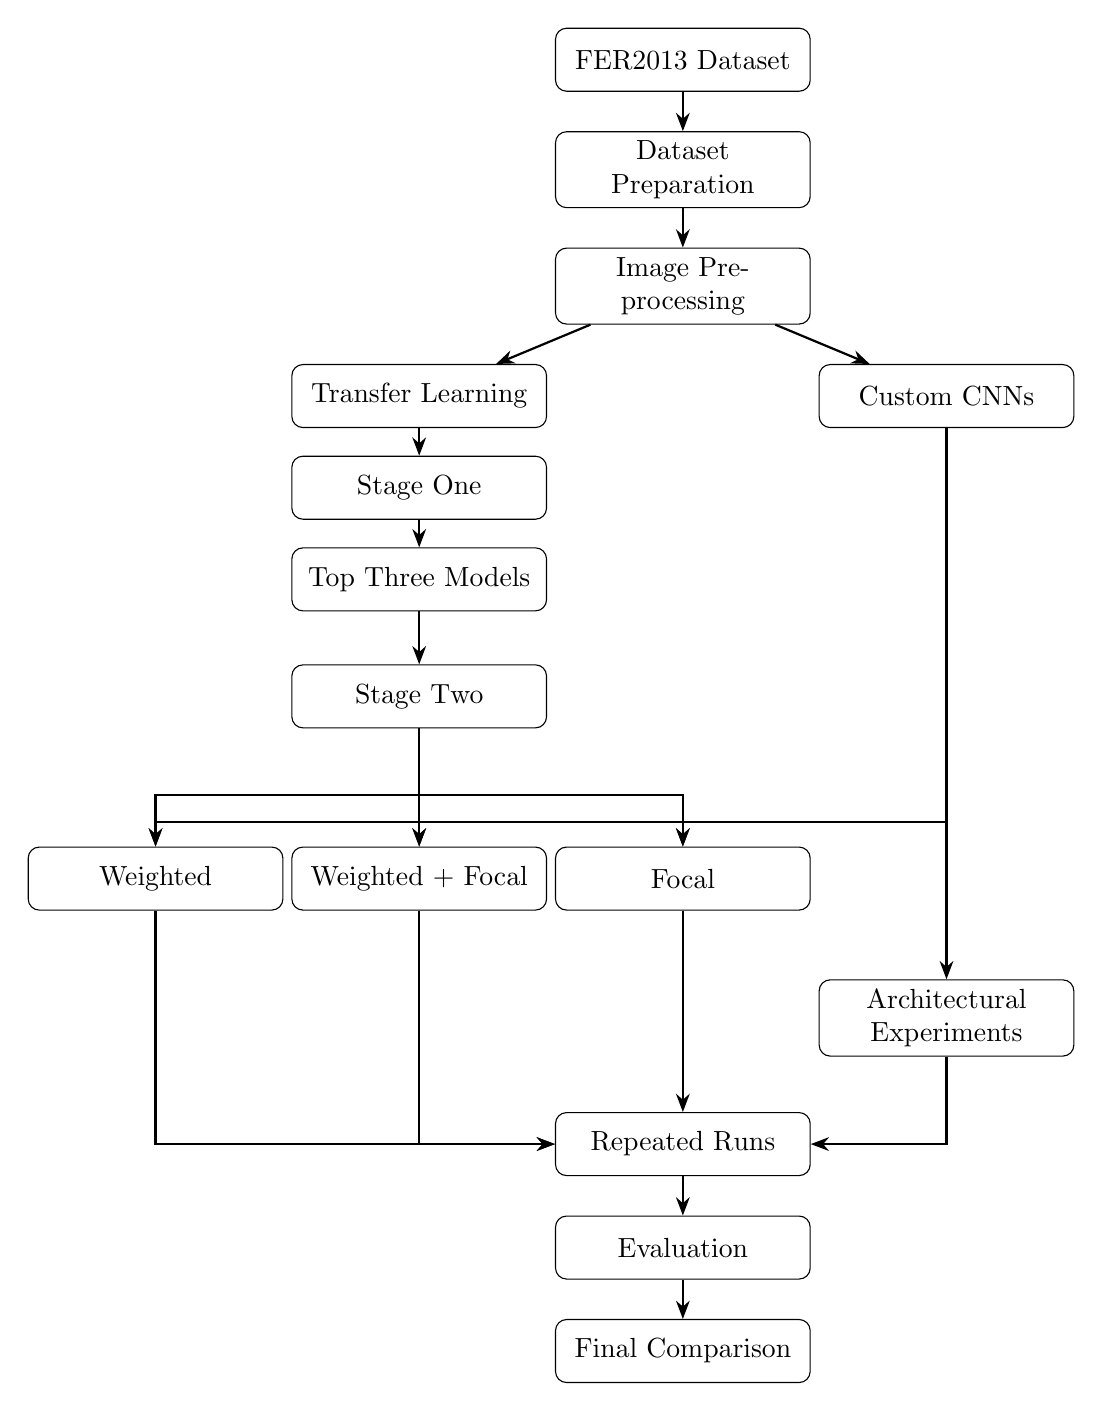
\begin{tikzpicture}[
					node distance=1.2cm,
					box/.style={
						rectangle,
						rounded corners,
						draw,
						text width=3cm,
						minimum height=0.8cm,
						align=center
					},
					arrow/.style={
						-{Stealth},
						thick
					}
				]

					\node[box] (dataset) {FER2013 Dataset};

					\node[box, below=0.5cm of dataset] (prep) {Dataset Preparation};

					\node[box, below=0.5cm of prep] (preprocess) {Image Preprocessing};

					\node[box, below right=0.5cm and 0.1cm of preprocess] (cnn) {Custom CNNs};
					
					\node[box, below=7cm of cnn] (experi) {Architectural Experiments};

					\node[box, below left=0.5cm and 0.1cm of preprocess] (tl) {Transfer Learning};

					\node[box, below=0.35cm of tl] (stageone) {Stage One};

					\node[box, below=0.35cm of stageone] (selection) {Top Three Models};

					\node[box, below=3cm of tl] (stagetwo) {Stage Two};
					
					\node[box, below left=1.5cm and 0.1cm of stagetwo] (weight) {Weighted};
					
					\node[box, below=1.5cm of stagetwo] (both) {Weighted + Focal};
					
					\node[box, below right=1.5cm and 0.1cm of stagetwo] (focal) {Focal};
					
					\node[box, below=10cm of preprocess] (runs) {Repeated Runs};

					\node[box, below=0.5cm of runs] (evaluation) {Evaluation};

					\node[box, below=0.5cm of evaluation] (comparison) {Final Comparison};

					\draw[arrow] (dataset) -- (prep);
					\draw[arrow] (prep) -- (preprocess);

					\draw[arrow] (preprocess) -- (cnn);
					\draw[arrow] (preprocess) -- (tl);

					\draw[arrow] (tl) -- (stageone);
					\draw[arrow] (stageone) -- (selection);
					\draw[arrow] (selection) -- (stagetwo);
					\draw[arrow] (stagetwo) -- ++(0,-1.25) -| (weight.north);
					\draw[arrow] (stagetwo) -- (both.north);
					\draw[arrow] (stagetwo) -- ++(0,-1.25) -| (focal.north);
					
					\draw[arrow] (weight) |- (runs.west);
					\draw[arrow] (both) |- (runs.west);
					\draw[arrow] (focal) -- (runs);

					\draw[arrow] (cnn) -- (experi);
					\draw[arrow] (cnn.south) -- ++(0,-5) -| (weight.north);
					\draw[arrow] (cnn.south) -- ++(0,-5) -| (both.north);
					\draw[arrow] (cnn.south) -- ++(0,-5) -| (focal.north);
					\draw[arrow] (experi) |- (runs);
					\draw[arrow] (runs) -- (evaluation);

					\draw[arrow] (evaluation) -- (comparison);

				\end{tikzpicture}}

				\caption{Overview of the Experimental Workflow used in the Investigation.}
				\label{fig:experimental_workflow}

			\end{figure}
			\newpage\mbox{}
			\newpage
			\subsection{Research Approach}
				
				The investigation can be characterised as a comparative experimental study. Model architecture and training strategy were treated as the principal experimental factors, while the dataset, preprocessing procedure, general optimisation conditions, and evaluation framework were kept consistent where possible. This allowed differences in model performance to be examined in relation to deliberate changes in architecture or training strategy rather than differences in the underlying dataset or evaluation procedure.\\\\
				The custom CNN experiments investigated the effect of architectural design choices by comparing four independently constructed CNN architectures. These architectures differed in aspects including network depth and size, convolutional filter configuration, data augmentation, regularisation, and the inclusion of residual connections. The resulting models provided a basis for examining whether progressively different architectural designs affected the ability of a CNN to generalise from the FER2013 training data to unseen data.\\\\
				Transfer learning provided a second architectural approach. VGG16, ResNet50, and InceptionV3 were used with pretrained ImageNet weights, with Stage One comparing configurations that differed in whether the pretrained feature extractor was frozen or partially fine-tuned and whether additional dense classification layers were included. Four layers were unfrozen in the fine-tuned configurations. This allowed the investigation to examine whether the choice of pretrained architecture and modifications to its classification head influenced performance on FER2013.\\\\
				Training strategy formed a separate experimental factor in Stage Two. The baseline training configuration used categorical cross-entropy without class weighting, while alternative configurations incorporated class weighting, focal loss, or both techniques. Class weighting was derived from the class frequencies of the FER2013 training subset, while focal loss was implemented using TensorFlow's \texttt{CategoricalFocalCrossentropy}. These strategies were investigated because the FER2013 classes are unevenly represented and therefore provide an opportunity to examine whether modifying the training objective could improve classification performance.\\\\
				The use of repeated training runs formed a further component of the experimental design. Every model configuration was trained five times using different random seeds. This allowed the stability of model performance to be examined across independent runs and reduced the likelihood that conclusions would depend on a single random initialisation. The results from these runs were subsequently summarised using their mean, standard deviation, minimum, and maximum values.
			\newpage
			\subsection{Experimental Comparisons}
			\label{sec:experimental_comparisons}
				
				The experimental comparisons were organised into three related stages. The first comparison examined the custom CNN architectures, the second examined alternative transfer-learning configurations, and the third examined alternative training strategies applied to the strongest transfer-learning configurations. This structure allowed architectural effects to be considered separately from the effects of the training strategies introduced in Stage Two.\\\\
				The custom CNN experiment compared four architectures: \texttt{Base\_CNN}, \texttt{CNN3}, \texttt{CNN4}, and \texttt{CNN5}. \texttt{Base\_CNN} provided the baseline architecture, while the subsequent configurations introduced progressively different architectural characteristics. These included changes to network size and structure, data augmentation, regularisation, and residual connections. The resulting performance was compared to determine whether these architectural modifications produced measurable differences in facial emotion recognition performance.\\\\
				The first stage of the transfer-learning experiment compared configurations based on VGG16, ResNet50, and InceptionV3 using pretrained ImageNet weights. Within these architectures, configurations differed according to whether the pretrained layers remained frozen or the final four layers were fine-tuned, and whether additional dense classification layers were included. This produced a set of transfer-learning configurations that could be ranked according to their performance.\\\\
				Following Stage One, the transfer-learning configurations were ranked primarily according to mean balanced accuracy. Where necessary, subsequent ranking criteria were applied in the following order: macro F1, mean validation accuracy, mean training time, and validation-accuracy standard deviation. The three highest-ranked configurations were selected for Stage Two. This procedure provided a consistent method for identifying the strongest transfer-learning configurations before changing the training strategy.\\\\
				Stage Two retained the underlying architectures of these three selected configurations while changing the training strategy. Each selected configuration was evaluated using class weighting, focal loss, and a combination of class weighting and focal loss. The resulting Stage Two models were compared not only with their corresponding baseline configurations but with the complete set of Stage One transfer-learning results. This allowed the effect of the alternative training strategies to be considered both within the selected architectures and in relation to the wider transfer-learning experiment.\\\\
				All configurations were evaluated using the same general testing and reporting procedure. Consequently, the first part of the investigation provided evidence concerning differences between CNN and transfer-learning architectures and their configurations, while the second provided evidence concerning the influence of alternative training strategies on selected transfer-learning models.

		\section{Dataset Preparation}
			
			The FER2013 dataset was used as the common dataset for all experiments. The FER2013 dataset was introduced as part of the Challenges in Representation Learning \cite{goodfellow2015challenges} and was subsequently used as the basis for the Facial Expression Recognition Challenge hosted on Kaggle \cite{fer2013_kaggle}. As the original Kaggle competition is no longer active, the copy of \texttt{fer2013.csv} used in this investigation was obtained from a separate Kaggle distribution of the dataset \cite{ahmed_fer2013_kaggle}. The CSV file contains grayscale facial images represented as space-separated pixel values, together with an integer emotion label and a `Usage' field identifying the predefined dataset partition.\\\\
				The original pixel representation was converted into normalised RGB image tensors before being supplied to the models. Labels were converted into one-hot encoded vectors to provide the target representation required for the seven-class softmax output layers. The same image preprocessing procedure was used for all models, with the exception that InceptionV3 internally resized its input to $75\times75$ pixels. Model-specific data augmentation was applied within the relevant custom CNN architectures rather than as part of the shared dataset pipeline.
			
			\subsection{Dataset Loading}
				
				The original \texttt{fer2013.csv} file was loaded using the pandas \texttt{read\_csv()} function. The `Usage' column was then used to identify the three predefined partitions supplied with the dataset. Rows labelled \textit{Training}, \textit{PublicTest}, and \textit{PrivateTest} were separated into the training, validation, and test data frames respectively.\\\\
				An additional label column was created by mapping the numerical emotion identifiers to their corresponding emotion names using the \texttt{EMOTION\_LOOKUP} mapping. The resulting data frames were also saved as separate CSV files for reproducibility and convenient inspection during development. However, the training procedure did not repeatedly reload these CSV files. The prepared data frames were retained in memory and supplied directly to the dataset creation function for each experimental run.\\\\
				This distinction is important because the saved CSV files represented persistent copies of the prepared dataset partitions, rather than separate datasets being generated or loaded for each training run.
				
			\newpage
			\subsection{Dataset Splitting}
				
				The dataset was divided according to the predefined FER2013 partitions into \texttt{train\_df}, \texttt{val\_df}, and \texttt{test\_df}. The \texttt{train\_df} subset, corresponding to the original \textit{Training} partition, was used to update the model parameters during training.\\\\
				The \texttt{val\_df} subset, corresponding to the original \textit{PublicTest} partition, was used to monitor model performance during training. Validation performance was used by the training procedure, including early stopping and learning-rate adjustment, but the validation examples were not directly used to update the model parameters.\\\\
				The \texttt{test\_df} subset, corresponding to the original \textit{PrivateTest} partition, was reserved for final evaluation. It was not used as the validation dataset during training or for the adaptive training decisions described elsewhere in this chapter.\\\\
				This separation ensured that training, validation-based model development, and final testing remained distinct. In particular, retaining the test partition for final evaluation reduced the risk of incorporating information from the final evaluation set into model development.
				
			\subsection{Image Preprocessing}
				
				The original FER2013 images were stored as space-separated pixel-value strings rather than as image tensors. \texttt{The load\_fer\_image()} function first split each pixel string into its individual values and converted them to 32-bit floating-point numbers.\\\\
				The resulting $2,304$ values were reshaped into a $48\times48\times1$ tensor, representing the original $48\times48$ grayscale image. The pixel values were subsequently divided by $255$, converting their original range of $[0,255]$ to the interval $[0,1]$. This normalisation provided the models with consistently scaled numerical inputs.\\\\
				The resulting grayscale image was then resized using the image dimensions configured in config.py. For the experiments described in this investigation, this remained $48\times48$ for the shared dataset pipeline. The image was subsequently converted from one channel to three channels using \texttt{tf.image.grayscale\_to\_rgb()}, producing an input tensor of shape $48\times48\times3$.\\\\
				The conversion to three channels allowed the same dataset representation to be supplied to both the custom CNN architectures and the pretrained transfer-learning architectures. This was particularly relevant to the VGG16, ResNet50, and InceptionV3 models, whose pretrained ImageNet architectures require three-channel image input.\\\\
				No model-specific ImageNet preprocessing function was applied after this conversion. Consequently, all models received the same normalised RGB representation from the shared dataset pipeline.\\\\\\
				For the InceptionV3 configurations, the $48\times48$ input was subsequently resized internally by the model to $75\times75$ pixels before being processed by the pretrained architecture. This resizing therefore formed part of the InceptionV3 model configuration rather than a modification to the shared FER2013 dataset pipeline.\\\\
				Model-specific data augmentation was also deliberately excluded from this preprocessing stage. Where augmentation was investigated, it was implemented within the relevant custom CNN architecture. This ensured that augmentation constituted an architectural/training configuration being evaluated rather than an alteration to the common dataset supplied to all models.
				
			\subsection{Label Encoding}
				
				The original emotion labels were represented by integer class identifiers corresponding to the seven FER2013 emotion categories: Angry, Disgust, Fear, Happy, Sad, Surprise, and Neutral.\\\\
				Within \texttt{load\_fer\_image()}, each integer label was converted into a one-hot encoded vector using \texttt{tf.one\_hot()} with a depth of seven. The resulting representation contained seven values, with the position corresponding to the correct emotion assigned a value of one and all other positions assigned zero.\\\\
				This representation matched the seven-unit softmax output layer used by the models and was compatible with the categorical loss functions used during training, including categorical cross-entropy and focal loss.
				
			\subsection{Dataset Pipeline}
				
				The prepared data frames were converted into TensorFlow tf.data.Dataset objects using \texttt{tf.data.Dataset.from\_tensor\_slices()}. The dataset was constructed from the `pixels' and `emotion' columns of each data frame, with the raw pixel strings and integer labels subsequently passed to \texttt{load\_fer\_image()}.\\\\
				The \texttt{map()} operation applied \texttt{load\_fer\_image()} to each sample in the dataset. Consequently, conversion of the pixel string, image reshaping, normalisation, RGB conversion, and one-hot label encoding were performed as part of the TensorFlow input pipeline rather than requiring the complete dataset to be converted and stored as image tensors in memory before training.\\\\
				The mapping operation used \texttt{num\_parallel\_calls=tf.data.AUTOTUNE}. The \\\texttt{num\_parallel\_calls} parameter allows multiple samples to be processed concurrently rather than requiring preprocessing to occur one sample at a time. Setting it to \texttt{tf.data.AUTOTUNE} allows TensorFlow to determine an appropriate degree of parallelism based on the execution environment.\\\\\\\\\\
				The training dataset was additionally shuffled using \texttt{shuffle(1000)}. Shuffling was applied only to the training dataset and not to the validation or test datasets. This randomised the order in which training examples were presented to the model, reducing the likelihood that the ordering of the source data would systematically influence training.\\\\
				The datasets were subsequently divided into mini-batches using the batch size specified for the current training run. The initial batch size for each model was configured according to the model's expected computational requirements. If a training run produced a \texttt{ResourceExhaustedError}, indicating that the available memory was insufficient, the batch size was halved and the failed run was retried using the reduced value. This process continued until the run succeeded or the predefined minimum batch size was reached.\\\\
				Finally, \texttt{prefetch(tf.data.AUTOTUNE)} was used to prepare future batches while the model was processing the current batch. Without prefetching, model execution may need to wait for the next batch to finish being prepared before continuing. Prefetching allows input preparation and model execution to overlap, reducing periods in which the model is waiting for data.\\\\
				Together, parallelised mapping and automatic prefetching allowed TensorFlow to perform input preparation concurrently with model execution where system resources permitted. This was intended to improve input-pipeline efficiency without changing the data supplied to the models.\\\\
				The resulting pipeline therefore provided each experiment with consistently processed FER2013 images and labels while allowing training data to be shuffled, batched, and prepared efficiently for model execution. The only deliberate variation in the dataset pipeline between runs was the batch size, which could be reduced automatically when memory constraints prevented successful training.
				
		\section{Custom CNN Architectures}
			
			Four custom convolutional neural network (CNN) architectures were developed specifically for facial emotion recognition rather than using existing pretrained architectures. All four models used the same $48 \times 48 \times 3$ input representation described in Section~\ref{sec:Experimental_Design}, with architectural changes introduced progressively during model development. The complete layer-by-layer configurations and output dimensions are provided in Appendix \ref{tab:base_cnn}--\ref{tab:cnn5}.\\\\
			The four architectures were not intended to provide isolated ablation studies of individual architectural components. Instead, they represent progressively modified CNN designs incorporating increased model capacity, regularisation, data augmentation and, in the final configuration, residual connections. Consequently, differences in performance between the architectures indicate the effect of the resulting model configurations as a whole rather than providing evidence for the independent effect of any single modification.\\\\
			Table \ref{tab:cnn_configurations} summarises the principal differences between the four architectures.\\
			\begin{table}[h!]
				\centering
				\caption{Custom CNN Model Configurations}
				\label{tab:cnn_configurations}
				\makebox[\textwidth]{
				\begin{tabular}{lp{4.0cm}p{3.0cm}p{2.0cm}p{2.0cm}}
					\toprule
					Model & Main architectural changes & Convolutional Structure & Data Augmentation & Residual connections \\
					\midrule
					Base\_CNN & Reference architecture with relatively low model capacity. & 7 convolutional layers & No & No \\
					CNN3 & Substantial increase in model capacity and introduction of spatial dropout. & 9 convolutional layers & No & No \\
					CNN4 & Introduction of data augmentation and a higher number of starting filters in first convolutional layer. & 5 convolutional layers & Yes & No \\
					CNN5 & Introduction of residual connections, and a more stable number of filters across convolutional layers & 7 convolutional layers, and 2 shortcut convolutional layers & Yes & Yes \\
					\bottomrule
				\end{tabular}}
			\end{table}\\
			The four CNN architectures were subsequently evaluated using the four training strategies described in Section~\ref{sec:Training_Strategies}: standard categorical cross-entropy, class weighting, focal loss, and a combination of class weighting and focal loss. Thus, the training strategy was varied independently of the choice of custom CNN architecture, with each architecture evaluated under each strategy.

			\subsection{Baseline CNN}
				
				The \texttt{create\_Base\_CNN()} function defines the baseline custom CNN architecture used as the reference point for the subsequent custom CNN configurations. The model accepts $48 \times 48 \times 3$ images and processes them through a sequence of convolutional, batch-normalisation, activation and pooling layers before producing a seven-class prediction.\\\\
				The initial convolutional layer uses two filters with a $10 \times 10$ kernel, followed by batch normalisation, ReLU activation and max pooling. Subsequent convolutional layers progressively increase the number of filters to eight while reducing the kernel sizes. Two further max-pooling operations reduce the spatial dimensions of the feature maps before global average pooling is applied. The complete architecture is shown in Appendix \ref{tab:base_cnn}.\\\\
				Global average pooling converts each final feature map into a single representative value. This produces an eight-dimensional representation which is passed to a dense layer containing $128$ ReLU-activated units before the final seven-unit softmax classification layer. Global average pooling was therefore used in preference to flattening the complete feature maps, substantially limiting the number of parameters entering the dense classifier.\\\\
				Batch normalisation is applied following each convolutional layer. The convolutional layers therefore use \texttt{use\_bias=False}, as the subsequent batch-normalisation layers provide the associated learned offset and scaling operations. This configuration was retained throughout the custom CNN architectures where batch normalisation followed the convolutional operation.\\\\
				The baseline provided a relatively small and simple CNN against which the progressively modified architectures could be compared.
				
			\subsection{Architectural Modifications}
				
				The subsequent CNN configurations were developed by increasing model capacity and incorporating additional mechanisms intended to improve the efficiency and generalisation of training. These changes were not designed as independent controlled experiments; rather, each architecture represented a particular combination of design decisions made during the development of the custom CNN models.\\\\
				CNN3 substantially increases the capacity of the baseline network. It uses nine convolutional layers and progressively increases the number of filters to $256$, compared with a maximum of eight filters in the baseline. Spatial dropout is introduced at several points within the feature extractor as the network becomes larger. The resulting architecture therefore combines substantially greater representational capacity with additional regularisation. The complete configuration is provided in Appendix \ref{tab:cnn3}.\\\\
				CNN4 adopts a different architecture with fewer convolutional layers but substantially larger numbers of filters from the outset. It also incorporates data augmentation and spatial dropout. The architecture therefore represents a more heavily regularised model with greater width than the baseline, rather than simply extending the depth of CNN3. Its complete configuration is given in Appendix \ref{tab:cnn4}.\\\\
				CNN5 extends this development by introducing residual connections while retaining several of the regularisation and augmentation mechanisms used in CNN4. Its architecture uses a main convolutional pathway together with shortcut pathways, allowing feature representations to bypass groups of convolutional operations. The complete structure, including the main and shortcut paths, is provided in Appendix \ref{tab:cnn5}.\\\\\\\\\\
				An incidental implementation difference between the architectures is that the first convolutional layer of Base\_CNN and CNN3 uses \texttt{padding=valid}, whereas the convolutional layers in CNN4 and CNN5 use \texttt{padding=same}. This difference was not itself established as an experimental variable and was a consequence of the architectural development process. It should therefore not be interpreted as an intentional comparison of padding strategies.
				
			\subsection{Data Augmentation}
				
				Data augmentation was incorporated directly into CNN4 and CNN5 rather than being permanently applied to the dataset during dataset preparation. The augmentation layers therefore formed part of the model architecture and generated modified training examples during model training.\\\\
				The same fixed set of transformations was used in both architectures: random horizontal flipping, random rotation, random zoom and random translation. These transformations were intended to expose the models to variation in facial orientation, position and scale that may occur in facial images.\\\\
				The augmentation was introduced as part of the broader development of the later CNN architectures rather than as an isolated experimental variable. Consequently, CNN4 and CNN5 cannot be used to determine the independent effect of augmentation alone, because their introduction was accompanied by other architectural and regularisation changes. Nevertheless, its inclusion formed part of the increasingly regularised model configurations evaluated in the custom CNN experiments.
				
			\subsection{Regularisation}
				
				Several regularisation and stabilisation techniques were incorporated into the custom CNN architectures as model complexity increased. These techniques were intended to improve training behaviour, reduce overfitting and produce more efficient architectures.\\\\
				Batch normalisation was applied after convolutional layers throughout the custom CNN architectures. In addition to its role in stabilising activation distributions during training, its use allowed the convolutional layers to be configured with \texttt{use\_bias=False}, since the subsequent batch-normalisation operation provides learned scaling and offset parameters \cite{ioffe2015batch}.\\\\
				Spatial dropout was introduced in CNN3 and retained in later architectures. Unlike conventional dropout, which independently removes individual activations, spatial dropout removes entire feature maps during training \cite{tompson2015efficient}. This was intended to reduce reliance on particular feature maps and encourage the development of more distributed representations as the convolutional feature extractors became larger.\\\\\\\\\\
				Standard dropout was also applied before the final classification layer in CNN4 and CNN5. This operates on individual activations in the dense representation and was used to reduce co-adaptation within the fully connected classification component \cite{srivastava2014dropout}.\\\\
				Global average pooling was used in all four architectures before the dense classification layers. By averaging each feature map across its spatial dimensions, the operation reduces the representation passed to the dense layers and avoids the substantially larger parameter count that would result from flattening the complete feature maps \cite{lin2014network}. This provided a consistent means of limiting the size of the final classifier across the custom CNN architectures.\\\\
				These regularisation and architectural components were introduced as part of the broader development and streamlining of the CNN models rather than being evaluated individually. Their combined use was intended to allow progressively more complex models to be trained while limiting unnecessary increases in parameter count and overfitting.
				
			\subsection{Residual Architecture}
				
				CNN5 introduced residual connections to investigate a different approach to constructing the convolutional feature extractor. Residual connections provide a shortcut through which the input representation of a block can bypass the convolutional operations before being combined with their output.\\\\
				Within CNN5, the main pathway applies convolutional and batch-normalisation operations before the resulting representation is combined with a shortcut pathway using an \texttt{Add()} operation. Where the number of feature maps changes between the input and output of a residual block, a $1 \times 1$ convolution is applied to the shortcut pathway to make the dimensions compatible. Batch normalisation is subsequently applied to the shortcut representation before the two pathways are combined.\\\\
				The resulting operation allows the original feature representation to be passed alongside the transformed representation. This provides an additional route for information and gradients through the network and can help the optimisation of deeper convolutional architectures.\\\\
				CNN5 combines the residual structure with several of the other design choices introduced during the custom CNN development, including data augmentation, batch normalisation, spatial dropout, global average pooling and standard dropout. It therefore represents a combined architectural configuration rather than an isolated experiment examining residual connections alone.\\\\
				The complete main and shortcut pathways of CNN5 are provided in Appendix \ref{tab:cnn5}.

		\section{Transfer Learning Architectures}
		\label{sec:transfer_learning_architectures}
			
			Transfer learning was investigated as an alternative to training custom CNN architectures entirely from the FER2013 dataset. Three established convolutional architectures pretrained on ImageNet were used: VGG16 \cite{simonyan2015vgg}, ResNet50 \cite{he2016resnet}, and InceptionV3 \cite{szegedy2016inception}. The architectures were selected as the pretrained models specified for the investigation and provided three established feature-extraction architectures against which the custom CNNs could be compared.\\\\
			For each architecture, the original classification component was excluded and replaced with a task-specific classifier for the seven FER2013 emotion classes. Global average pooling was applied to the output of each pretrained convolutional base. Stage One then varied two related configuration choices: whether the pretrained base remained fully frozen or its final four layers were made trainable, and whether the trainable-base configuration used an additional classification head consisting of two 256-unit dense layers. The two dense layers were treated as a single classification-head configuration rather than as separate architectural modifications.\\
				\begin{table}[h!]
					\centering
					\caption{Transfer Learning Model Configurations}
					\label{tab:tl_configurations}
					\begin{tabularx}{\textwidth}{lXX}
						\toprule
						Model & Fine-tuning configuration & Additional dense layers \\
						\midrule
						VGG16\_Frozen & fully frozen & no additional layers \\
						VGG16\_Unfreeze4 & last 4 layers unfrozen & no additional layers \\
						VGG16\_Unfreeze4\_Head & last 4 layers unfrozen & two 256 layers \\
						ResNet50\_Frozen & fully frozen & no additional layers \\
						ResNet50\_Unfreeze4 & last 4 layers unfrozen & no additional layers \\
						ResNet50\_Unfreeze4\_Head & last 4 layers unfrozen & two 256 layers \\
						InceptionV3\_Frozen & fully frozen & no additional layers \\
						InceptionV3\_Unfreeze4 & last 4 layers unfrozen & no additional layers \\
						InceptionV3\_Unfreeze4\_Head & last 4 layers unfrozen & two 256 layers \\
						\bottomrule
					\end{tabularx}
				\end{table}\\
				The nine configurations in Table \ref{tab:tl_configurations} constituted Stage One of the transfer-learning investigation. The complete transfer-learning configurations, including the Stage Two training strategies, are provided in Appendix \ref{tab:all_tl_configurations}. Stage Two introduced no further architectural changes. Instead, the three highest-ranked Stage One configurations, selected according to the model-selection procedure described in Section~\ref{sec:Selection_of_Transfer_Learning_Models_for_Stage_Two}, were retrained using the alternative training strategies described in Section~\ref{sec:Training_Strategies}.
				
			\newpage
			\subsection{VGG16}
				
				VGG16 was used as the first pretrained transfer-learning architecture. Its convolutional base was initialised using ImageNet pretrained weights, with the original classification component excluded. The resulting feature representation was passed through global average pooling before being connected to the seven-class FER2013 classifier.\\\\
				Two configurations were evaluated with the VGG16 base: a fully frozen configuration and a configuration in which the final four layers were made trainable. A further configuration combined the latter with the additional classification head consisting of two 256-unit dense layers. Thus, the VGG16 experiments examined the effect of making the final pretrained layers trainable and, separately within that configuration, increasing the capacity of the classification head.
				
			\subsection{ResNet50}
				
				ResNet50 was used as the second pretrained transfer-learning architecture. Its ImageNet-pretrained classification component was excluded and replaced with the same task-specific classification structure used for the VGG16 experiments.\\\\
				ResNet50 incorporates residual connections, which provide alternative paths through the network for information and gradients. This architectural characteristic distinguishes it from the VGG16 architecture while requiring no additional modification to the pretrained network for the purposes of this investigation.\\\\
				As with VGG16, Stage One evaluated a fully frozen configuration, a configuration with the final four layers made trainable, and a configuration combining the latter with two additional 256-unit dense layers.
				
			\subsection{InceptionV3}
				
				InceptionV3 was used as the third pretrained transfer-learning architecture. Its convolutional base was initialised using ImageNet pretrained weights and its original classification component was replaced with the seven-class FER2013 classifier.\\\\
				Unlike the VGG16 and ResNet50 implementations, the InceptionV3 model included an internal resizing operation. The common dataset representation remained $48 \times 48 \times 3$, but the input was resized to $75 \times 75 \times 3$ within the InceptionV3 model before being passed to the pretrained architecture. This was necessary because the TensorFlow/Keras implementation of InceptionV3 used in the investigation has a minimum spatial input size of $75 \times 75$.\\\\
				The same three Stage One configuration types were then evaluated for InceptionV3: a fully frozen base, a base with its final four layers made trainable, and the latter configuration with two additional 256-unit dense layers.

			\subsection{Layer Freezing and Fine-tuning}
				
				The transfer-learning experiments used layer freezing to control the extent to which the pretrained representations were changed during training. In the fully frozen configurations, the parameters of the pretrained convolutional base were retained from ImageNet pretraining and were not updated using FER2013. The newly added task-specific classification layers remained trainable.\\\\
				A second configuration for each architecture selected the final four layers of the pretrained base for fine-tuning. In the implementation, any BatchNormalization layers within this group were kept frozen; the remaining selected layers were made trainable. This allowed a limited portion of the pretrained representation to adapt to FER2013 while retaining the majority of the ImageNet-derived feature extractor. This configuration is referred to as `Unfreeze4' throughout the investigation to distinguish it clearly from the fully frozen models.\\\\
				The third configuration combined this same four-layer unfreezing strategy with an additional classification head consisting of two 256-unit dense layers. No configurations combining a fully frozen base with the additional dense head were evaluated.\\\\
				The Stage One configurations therefore provided a structured comparison of pretrained feature extraction, limited adaptation of the pretrained base, and increased classification-head capacity. Following Stage One, the three highest-ranked configurations were selected using the model-selection procedure described in Section~\ref{sec:Selection_of_Transfer_Learning_Models_for_Stage_Two}. These architectures were then retained unchanged for Stage Two, where the effects of alternative training strategies were investigated.
				
		\section{Training Procedure}
			
			The custom CNN and transfer-learning models were trained using a common training framework wherever possible. Consistent optimisation settings, stopping criteria, repeated runs and evaluation procedures were used so that differences in performance could be considered in relation to the architectural and training choices being investigated rather than substantially different training conditions. The complete model configurations are provided in Appendix \ref{tab:all_cnn_configurations} and Appendix \ref{tab:all_tl_configurations}.\\\\
			Models were trained using the FER2013 training dataset and monitored using the validation dataset during training. The held-out test dataset was not used during training, validation, model selection or callback-based decisions. It was used only after a model had completed training and validation, to obtain its final test-set performance. Each model configuration was trained for five successful runs using different random seeds, with the resulting metrics summarised across the successful runs.
			
			\subsection{Optimisation}
				
				The AdamW optimiser was used for the final model training experiments. Before the final experiments, approximately three to four complete runs of the CNN comparison code were performed using the Adam optimiser, with one run per model configuration. These preliminary runs were used to assess whether there were substantial differences in training speed or classification performance between the two optimisers. The preliminary experiments were conducted before the training timer was introduced and therefore did not provide directly comparable quantitative training-time measurements. However, no substantial differences in classification accuracy were observed, while AdamW appeared to complete the experiments more quickly overall. AdamW was therefore adopted for the subsequent experiments.\\\\
				AdamW combines the adaptive parameter-update behaviour of Adam with decoupled weight decay \cite{loshchilov2019decoupled}. A weight decay value of $1 \times 10^{-4}$ was used throughout the experiments. The remaining optimiser parameters were left at the defaults provided by the TensorFlow version used for the investigation.\\\\
				Using the same optimiser and weight-decay setting across the experiments provided a common optimisation procedure for both the custom CNN and transfer-learning models.
				
			\subsection{Learning Rate}
				
				The initial learning rate was set to $1 \times 10^{-4}$ for all model configurations. This provided a common starting point for both the custom CNN and transfer-learning experiments.\\\\
				The learning rate was subsequently allowed to change during training using the \texttt{ReduceLROnPlateau} callback. This allowed progressively smaller parameter updates to be used when validation loss stopped improving, while retaining the same initial learning rate across the experiments.
				
			\subsection{Early Stopping}
				
				Training was configured with a nominal maximum of $1,000$ epochs. This limit was deliberately set considerably higher than the number of epochs generally expected to be required, allowing the callback-based stopping criteria to determine when further training was no longer beneficial.\\\\
				Early stopping monitored validation loss with a patience of $10$ epochs. If validation loss failed to improve for the specified period, training was stopped and the model weights were restored to those associated with the lowest validation loss observed during that run.\\\\
				None of the successful final runs reached the 1,000-epoch limit, with training generally terminating earlier as a result of the stopping criteria.
				
			\subsection{Learning Rate Reduction}
				
				The \texttt{ReduceLROnPlateau} callback monitored validation loss during training. When validation loss failed to improve for five consecutive epochs, the learning rate was reduced by a factor of $0.5$. A minimum learning rate of $1 \times 10^{-6}$ was used to prevent the learning rate from becoming arbitrarily small.\\\\
				This allowed training to begin with the common initial learning rate while progressively reducing the magnitude of parameter updates when improvement in validation loss reached a plateau.
				
			\subsection{Batch Size}
					
				Batch size was configured separately for each model configuration according to the available computational resources. The initial batch sizes could therefore differ between architectures. The batch size was also treated as an adaptive parameter during repeated training because some model configurations could exceed the available GPU memory at their initial setting. Further information about the computational environment is provided in Section~\ref{sec:computational_limits}.\\\\
				If TensorFlow raised a \texttt{ResourceExhaustedError} during a training run, the failed run was discarded and the current batch size was halved. The training procedure then recreated the training, validation and test datasets using the reduced batch size and retried the same run using the same random seed. The training dataset was shuffled when recreated, while the validation and test datasets were not shuffled.\\\\
				This process continued until the run completed successfully or the batch size reached the predefined minimum of four. Consequently, the final batch size could differ from the initially specified value for a particular model configuration. The batch size used by each successful run was recorded alongside the other training results.\\\\
				Training time included the time spent on failed batch-size attempts as well as the subsequent successful training and evaluation. For example, if a model produced an out-of-memory error after $30$ seconds at one batch size and then completed successfully after a further $120$ seconds at a lower batch size, the recorded training time for that run included the full 150 seconds.
					
			\subsection{Dataset Pipeline}
				
				The training, validation and test datasets were recreated for each model run using the corresponding dataframes and the current batch size. The image preprocessing pipeline converted the FER2013 pixel strings into normalised RGB images before batching. Pixel values were converted from the original $[0,255]$ range to $[0,1]$ within the \texttt{load\_fer\_image()} function, and the integer emotion labels were converted into seven-element one-hot encoded vectors.\\\\\\
				The resulting TensorFlow datasets were created using\\ \texttt{tf.data.Dataset.from\_tensor\_slices()} and processed using a single \texttt{.map()} operation. The mapping function applied the image conversion, normalisation, resizing specified by the configuration and grayscale-to-RGB conversion before returning the image and one-hot encoded label. No additional dataset-level augmentation was applied through the dataset pipeline. Data augmentation was instead incorporated directly into the selected custom CNN architectures.\\\\
				Only the training dataset was shuffled. The validation and test datasets were kept in a fixed order. Because the datasets were recreated for every run and for each batch-size retry, the training dataset was reshuffled whenever a new run or batch size was started. No additional shuffling was performed elsewhere in the training procedure.
				
			\subsection{Prefetching and Automatic Parallelism}
				
				The dataset pipeline used \texttt{tf.data.AUTOTUNE} both when mapping the preprocessing function and when prefetching batches. \texttt{AUTOTUNE} allows TensorFlow to determine suitable values for the amount of parallel preprocessing and the number of batches to prepare in advance based on the execution environment.\\\\
				The \texttt{prefetch()} operation allowed preparation of future batches to occur while the model was processing the current batch. This can reduce the amount of time the accelerator spends waiting for the next batch of data to become available. The use of parallel mapping and prefetching was therefore intended to improve the efficiency of the input pipeline without requiring manually selected parallelism or buffer settings.
				
			\subsection{Number of Training Runs}
				
				Each model configuration was trained for five successful runs in the final experiments. Repeating the training process reduced the influence of a single random initialisation and provided multiple observations from which the variability of model performance could be assessed.\\\\
				The results from the five successful runs were summarised using the mean, standard deviation, minimum and maximum values for the recorded metrics. This provided a broader description of model performance than relying on a single training run.\\\\
				The number of repetitions was constrained by the computational resources available for the investigation. A larger number of runs could provide additional information about performance variability, but would also substantially increase the computational cost.
				
			\newpage
			\subsection{Random Seeds}
				
				A predefined collection of random seeds was used to provide different random initialisation conditions between repeated runs. Before each run, the selected seed was used to control the relevant Python, NumPy and TensorFlow random-number generators.\\\\
				Using different seeds allowed repeated runs to begin from different random states while maintaining a reproducible experimental procedure. The same seed was retained when a run had to be retried following a GPU memory error, so the reduced-batch-size attempt represented a retry of the same run rather than a new random replicate.\\\\
				The number of available seeds also placed an upper limit on the number of distinct runs that could be requested. The maximum possible value of \texttt{num\_runs} was therefore equal to the number of seeds defined in the project's \texttt{SEEDS} list, which contained 20 seeds.
				
		\section{Training Strategies}
		\label{sec:Training_Strategies}
			
			In addition to architectural differences, the investigation examined the influence of different training strategies on model performance. These experiments changed the loss function and/or the use of class weighting while keeping the principal architectural and common training conditions unchanged. The complete combinations used for the custom CNN models are provided in Appendix \ref{tab:all_cnn_configurations}.\\\\
			The custom CNN architectures were each trained using four strategies: baseline categorical cross-entropy, categorical cross-entropy with class weighting, focal loss, and focal loss combined with class weighting. For transfer learning, Stage Two evaluated the three alternative strategies of class weighting, focal loss, and their combination for the selected models. The Stage Two transfer-learning experiments therefore did not explicitly repeat the baseline categorical cross-entropy condition.
			
			\subsection{Baseline Training}
				
				The baseline training strategy used categorical cross-entropy as the loss function without class weighting. This provided the reference training condition against which the alternative strategies could be compared.\\\\
				Categorical cross-entropy measures the difference between the true one-hot encoded class distribution and the probability distribution predicted by the model. Predictions assigning a low probability to the correct class therefore contribute more strongly to the loss.\\\\
				No additional weighting was applied to individual emotion classes under the baseline strategy, so each training example contributed according to the standard categorical cross-entropy formulation.
				
			\subsection{Class Weighting}
				
				Class weighting was introduced to account for the imbalance between the seven emotion classes in FER2013. The number of training examples differs substantially between the classes, meaning that unweighted training provides considerably more examples from some emotions than from others.\\\\
				Class weights were calculated once using the balanced weighting approach provided by \texttt{compute\_class\_weight()} from scikit-learn. The resulting weights were then used consistently in the relevant weighted training configurations.\\
				\begin{table}[h!]
					\centering
					\caption{Class Weights Used During Training}
					\label{tab:class_weights}
					\makebox[\textwidth]{
					\begin{tabular}{lccr}
						\toprule
						Emotion & Class identifier & Number of training examples & Class weight \\
						\midrule
						Angry & 0 & 3995 & 1.0266046844269623 \\
						Disgust & 1 & 436 & 9.406618610747051 \\
						Fear & 2 & 4097 & 1.0010460615781582 \\
						Happy & 3 & 7215 & 0.5684387684387684 \\
						Sad & 4 & 4830 & 0.8491274770777877 \\
						Surprise & 5 & 3171 & 1.293372978330405 \\
						Neutral & 6 & 4965 & 0.8260394187886635 \\
						\bottomrule
					\end{tabular}}
				\end{table}\\
				The weights increased the contribution of errors involving under-represented classes and reduced the relative contribution of errors involving highly represented classes. Class weighting was therefore intended to reduce the extent to which the loss was dominated by the more frequent emotion categories and to encourage more balanced performance across the seven classes.
				
			\subsection{Focal Loss}
				
				Focal loss was investigated as an alternative to standard categorical cross-entropy \cite{lin2017focal}. It modifies the contribution of individual training examples so that confidently classified examples contribute less to the loss while difficult examples retain greater influence.\\\\
				This was relevant to facial emotion recognition because some emotion classes and individual examples can be difficult to distinguish from one another. Reducing the relative contribution of examples that the model already classifies confidently allows greater emphasis to be placed on examples that remain difficult to classify.\\\\
				The \texttt{CategoricalFocalCrossentropy} loss function provided by TensorFlow was used for the focal-loss experiments, with the default parameters supplied by the installed TensorFlow version. Unlike class weighting, focal loss primarily changes the contribution of examples according to classification difficulty rather than their class frequency.
				
			\subsection{Combined Class Weighting and Focal Loss}
				
				The final custom CNN training strategy combined class weighting with focal loss. Class weighting increased the contribution of under-represented classes, while focal loss reduced the relative contribution of confidently classified examples and emphasised more difficult examples.\\\\
				The same class-weight values used in the class-weighting experiments were supplied alongside the categorical focal loss function. This allowed the combined strategy to investigate whether addressing both class imbalance and example difficulty could provide benefits beyond either strategy individually.
				
		\section{Model Selection}
			
			Model selection was used to determine which transfer-learning configurations progressed from Stage One to Stage Two. The purpose was to avoid applying every possible training-strategy combination to every transfer-learning architecture, which would have substantially increased the computational cost of the investigation.\\\\
			The Stage One selection process used a comparison table that combined repeated-run summaries with classification-report metrics from each configuration's validation-selected best run. Mean balanced accuracy, mean validation accuracy, mean training time and validation-accuracy standard deviation summarised repeated-run results, while Macro F1 came from the test-set classification report for the selected best run. The selection therefore considered several dimensions of performance, but it was not based exclusively on repeated-run averages.
			
			\subsection{Selection of Transfer Learning Models for Stage Two}
			\label{sec:Selection_of_Transfer_Learning_Models_for_Stage_Two}
				
				The Stage One transfer-learning results were collected into a comparison table containing the mean validation accuracy, mean test accuracy, mean balanced accuracy, macro-averaged precision, macro-averaged recall, macro-averaged F1-score, weighted F1-score, validation accuracy standard deviation and mean training time.\\\\
				The saved comparison table was sorted using the following criteria, in descending priority:
				\begin{enumerate}
					\item Mean Balanced Accuracy, descending;
					\item Macro F1, descending;
					\item Mean Validation Accuracy, descending;
					\item Mean Training Time, ascending;
					\item Validation Accuracy Standard Deviation, ascending.\\\\
				\end{enumerate}
				No single metric was treated as a universally principal measure of model quality. Instead, the ordering provided a consistent procedure that considered class-balanced performance first, followed by additional measures of classification performance, computational cost and consistency.\\\\
				Stage Two automatically accessed the saved sorted Stage One comparison file and selected the first three entries using \texttt{.head(3)}. There was therefore no manual selection of the Stage Two models. Each selected transfer-learning configuration was subsequently retrained using class weighting, focal loss and the combination of class weighting and focal loss.
				
			\subsection{Selection of Best-performing Runs}
				
				Although each model configuration was trained repeatedly, the detailed classification report and confusion matrix were generated using the best-performing run for that configuration. The best run was selected according to its maximum validation accuracy. During each model's repeated runs, the current validation accuracy was compared against the best validation accuracy recorded so far, and a run was retained as the new best run only when its validation accuracy was strictly greater than the previous best value.\\\\
				Consequently, if two runs achieved exactly the same highest validation accuracy, the first run to achieve that value was retained. No additional tie-breaking procedure was applied.\\\\
				Only the history associated with the selected best run was retained for subsequent detailed analysis, together with the corresponding model outputs required for the classification report and confusion matrix. This distinction allowed model configurations to be compared using aggregate results across all successful runs while the later class-level analysis focused on the strongest validated run for each configuration.
				
		\section{Evaluation Procedure}
			
			The outputs produced during model training were converted into quantitative measures of classification performance and computational cost. These measures provided several complementary perspectives from which the architectures and training strategies could be compared.\\\\
			Evaluation considered both overall and class-balanced classification performance. This was particularly relevant to FER2013 because the seven emotion classes are not equally represented.
			
			\newpage
			\subsection{Performance Metrics}
				
				Several performance metrics were used to provide different perspectives on model behaviour. Accuracy measures the proportion of predictions assigned to the correct emotion class, while balanced accuracy gives equal importance to each class by calculating the average recall across the classes.\\\\
				Precision measures the proportion of predictions assigned to a particular class that were correct, while recall measures the proportion of actual examples belonging to that class that were correctly identified. The F1-score provides a combined measure of precision and recall.\\\\
				Macro-averaged precision, recall and F1-score were used to give each emotion class equal importance when summarising classification performance. Weighted F1-score was also recorded, with the contribution of each class weighted according to its number of examples. The complete set of metrics used in the investigation is summarised in Table \ref{tab:performance_metrics}.\\
				\begin{longtable}[c]{p{2.0cm}p{3.0cm}p{4.0cm}p{4.0cm}}
					\caption{Performance Metrics Used in the Investigation}
					\label{tab:performance_metrics}\\
					\toprule
					Metric & Definition & What it measures & Why it was used \\
					\midrule
					\endfirsthead
					\multicolumn{4}{c}%
					{{\tablename\ \thetable{} -- continued from previous page}} \\
   					\toprule
 					Metric & Definition & What it measures & Why it was used \\
 					\midrule
   					\endhead
  					\midrule
  					\multicolumn{4}{r}{{Continued on next page}} \\
  					\endfoot
   					\bottomrule
  					\endlastfoot
					Validation Accuracy & Proportion of correctly classified validation examples. & Performance on unseen validation data. & Used to compare repeated runs and select the best-performing run. \\
					Test Accuracy & Proportion of correctly classified test examples. & Overall classification performance on the held-out test set. & Provides a straightforward measure of final model performance. \\
					Balanced Accuracy & Mean recall across the seven emotion classes. & Class-balanced classification performance. & Accounts for the imbalance in FER2013. \\
					Macro Precision & Unweighted mean precision across classes. & Reliability of predictions across all emotion classes equally. & Assesses class-level prediction reliability without allowing frequent classes to dominate. \\
					Macro Recall & Unweighted mean recall across classes. & Ability to identify examples from each emotion class equally. & Assesses whether minority emotions are being identified effectively. \\
					Macro F1 & Unweighted mean F1 score across classes. & Balance between precision and recall across classes. & Provides a class-balanced combined performance measure. \\
					Weighted F1 & F1 score weighted by class frequency. & Precision-recall performance while accounting for class distribution. & Provides a complementary measure reflecting the actual dataset distribution. \\
					Validation accuracy standard deviation & Standard deviation of validation accuracy across repeated runs. & Variation in model performance between random seeds. & Assesses the consistency and stability of training outcomes. \\
					Training time & Elapsed time required to train the model. & Computational time required by each model. & Allows classification performance to be considered alongside computational cost. \\
					Efficiency score & Mean balanced accuracy divided by mean training time. & Classification performance relative to training time. & Provides a comparative measure of performance versus computational cost. \\
				\end{longtable}
				\noindent
				Balanced accuracy was given particular consideration when comparing models because the FER2013 classes are imbalanced. A model achieving high overall accuracy can still perform poorly on less frequent emotions, whereas balanced accuracy gives each emotion class equal influence on the resulting score. However, no single metric was treated as sufficient to assess overall model quality, and the different metrics were considered together.\\\\
				The F1 score is the harmonic mean of precision and recall. It therefore provides a combined measure that requires both quantities to be reasonably high. Macro F1 was calculated as the unweighted mean of the seven class-level F1 scores, giving each emotion equal influence regardless of its frequency.\\\\
				Weighted F1 was calculated by weighting each class-level F1 score according to the number of samples belonging to that class. It therefore provides a complementary measure that reflects the actual class distribution while still incorporating both precision and recall.\\\\
				Validation accuracy was used to select the best-performing run for each configuration, while validation loss controlled early stopping and learning-rate reduction. After each successful run, the test dataset was used to calculate test loss, test accuracy and balanced accuracy. Predictions from the validation-selected best run were then used to generate its classification report and confusion matrix. Test-derived metrics subsequently informed the Stage One selection of transfer-learning configurations and the final comparison and composite ranking. Consequently, although test data did not influence gradient updates or callback behaviour, it did influence later model selection and comparative ranking.
				
			\subsection{Confusion Matrices}
				
				Confusion matrices were generated to examine the distribution of predictions across the seven emotion classes. Rather than using raw counts, the matrices were normalised by the true class using \texttt{normalize="true"} in scikit-learn. The resulting values therefore represent the proportion of examples within each actual emotion category that were assigned to each predicted category.\\\\
				The diagonal elements represent the proportion of examples correctly classified for each emotion, while off-diagonal elements show the proportions incorrectly assigned to other emotions. The seven emotion classes were maintained in the same order for each confusion matrix, allowing the matrices to be compared directly.\\\\
				A confusion matrix was generated and saved for every model configuration using its selected best-performing run. These matrices were subsequently used in the CNN and Stage Two notebooks to examine class-specific performance and recurring patterns of confusion between emotions. This provided information that could not be obtained from aggregate metrics alone.
				
			\subsection{Classification Reports}
				
				Classification reports were generated using scikit-learn's \texttt{classification\_report()} function for the selected best-performing run of each model configuration. The reports provided class-level precision, recall and F1-score together with macro- and weighted-average results.\\\\
				These class-level results complemented the aggregate comparison metrics and confusion matrices by allowing the performance of individual emotion categories to be examined directly.
				
			\subsection{Training Time}
				
				Training time was recorded for each successful model run using a high-resolution performance timer. The measured interval covered both the model-training procedure and the subsequent evaluation performed by \texttt{evaluate\_trained\_model()}. Consequently, the recorded value represented the computational time required to train and evaluate the run rather than the duration of the \texttt{fit()} operation alone.\\\\
				If a run produced a GPU out-of-memory error and was subsequently retried at a lower batch size, the time spent on the failed attempt was also included in the recorded training time. The failed attempt was discarded as a training result, but its elapsed time remained part of the computational cost associated with successfully completing that run.\\\\\\\\\\\\
				Training time was measured exclusively in seconds throughout the investigation. Mean training time across the successful runs was used when comparing the computational cost of model configurations. OOM events were substantially less common for the transfer-learning experiments because the transfer-learning implementation was divided into separate Stage One and Stage Two notebook execution stages, reducing the amount of transfer-learning experimentation being run simultaneously.
				
			\subsection{Efficiency Score}
				
				An efficiency score was calculated for the model comparison tables as:\\
				\begin{align*}
					\text{Efficiency Score}&=\frac{\text{Mean Balanced Accuracy}}{\text{Mean Training Time}}
				\end{align*}\\
				The score combines classification performance with computational cost, with larger values indicating greater balanced accuracy achieved per second of recorded training and evaluation time.\\\\
				The efficiency score was calculated from the mean balanced accuracy and mean training time recorded for each model configuration and was stored in the model comparison CSV files. It was not calculated separately for individual runs, and consequently no mean, standard deviation, minimum or maximum efficiency score was calculated across runs.\\\\
				The efficiency score was not intended to replace classification metrics such as balanced accuracy or F1-score. It is a study-specific derived measure rather than a universally established machine-learning evaluation metric, and was used to examine the trade-off between classification performance and computational cost among the architectures investigated.
				
	\chapter{Results}
		
		\section{Custom CNN Results}
			
			The four custom convolutional neural network architectures were evaluated to examine how differences in architectural design and training configuration affected facial emotion recognition performance on the FER2013 dataset. The architectures comprised the Base CNN, CNN3 (Expanded), CNN4 (Augmentation), and CNN5 (Residual). Each architecture was evaluated using the four training configurations described previously: the baseline categorical cross-entropy configuration, class weighting, focal loss, and a combination of class weighting and focal loss. Consequently, 16 custom CNN configurations were evaluated in total.\\\\
			The results are presented in stages. First, the strongest configuration obtained for each architecture is compared to provide an architecture-level assessment. The relationship between architectural depth, filter capacity and observed performance is then examined using the base configuration of each architecture. This distinction is important because the architecture-level comparison identifies the strongest overall configuration for each architecture, whereas the depth and filter comparison is intended to assess the architectures themselves without selecting the configuration that happened to produce the best performance. The effects of the different training strategies are subsequently examined across the custom CNN configurations.
			
			\subsection{Overall CNN Performance}
				
				The overall performance of the four custom CNN architectures is summarised in Table \ref{tab:best_cnn_config}. For each architecture, the configuration with the highest mean balanced accuracy was selected for this architecture-level comparison. The results show a clear difference in performance between the architectures. The Base CNN achieved a mean validation accuracy of 0.4003, mean test accuracy of 0.3972 and mean balanced accuracy of 0.3152. CNN3 achieved higher values of 0.4342, 0.4342 and 0.3499, respectively. The strongest results were obtained by CNN4 and CNN5, with CNN4 achieving mean validation accuracy of 0.4853, mean test accuracy of 0.4977 and mean balanced accuracy of 0.4124, while CNN5 achieved corresponding values of 0.4997, 0.5053 and 0.4240.\\\\
				CNN5 therefore achieved the highest mean validation accuracy, mean test accuracy and mean balanced accuracy among the four architectures when considering their strongest configurations. Its Macro F1 of 0.4164 was also marginally higher than the 0.4155 obtained by CNN4. CNN3 and the Base CNN produced lower Macro F1 values of 0.3642 and 0.3072, respectively. Thus, the ordering of the architectures was broadly similar across the accuracy-based and macro-averaged measures, although the difference between CNN4 and CNN5 was comparatively small in terms of Macro F1.\\\\
				The results therefore demonstrate substantial variation in performance between the custom CNN architectures. The difference in mean balanced accuracy between the weakest architecture-level result, obtained by the Base CNN, and the strongest, obtained by CNN5, was approximately \num[round-precision=4]{0.108821553}, while the corresponding difference in mean test accuracy was approximately \num[round-precision=4]{0.10816384}. These differences provide an initial indication that the complete architectural configurations produced materially different levels of classification performance. However, because the architectures differed in several respects simultaneously, these results should be interpreted as comparisons between complete architectures rather than evidence that any individual architectural component was responsible for the observed differences.\\
				\begin{table}[h!]
					\centering
					\caption{Best CNN Model Configurations}
					\label{tab:best_cnn_config}
					\makebox[\textwidth]{
					\begin{tabular}{
						ll
						S[table-format=1.4, round-precision=4]
						S[table-format=1.4, round-precision=4]
						S[table-format=1.4, round-precision=4]
						S[table-format=1.4, round-precision=4]
					}
						\toprule
						Architecture & Best configuration & 
						\multicolumn{1}{>{\centering\arraybackslash}p{1.5cm}}{Mean Val. Acc.} & 
						\multicolumn{1}{>{\centering\arraybackslash}p{1.5cm}}{Mean Test Acc.} & 
						\multicolumn{1}{>{\centering\arraybackslash}p{1.5cm}}{Mean Bal. Acc.} & 
						\multicolumn{1}{>{\centering\arraybackslash}p{1.5cm}}{Macro F1}\\
						\midrule
						Base CNN & Base\_CNN\_Model & 0.400278628 & 0.397157985 & 0.315166145 & 0.307191838 \\
						CNN3 & CNN\_Model\_Expanded\_fnloss & 0.434159935 & 0.43415994 & 0.349868297 & 0.364247622 \\
						CNN4 & CNN\_Model\_Augmentation & 0.485316241 & 0.497743106 & 0.41240378 & 0.415537824 \\
						CNN5 & CNN\_Model\_Residual\_fnloss & 0.499749231 & 0.505321825 & 0.423987698 & 0.416388939 \\
						\bottomrule
					\end{tabular}}
				\end{table}\\
				
			\subsection{Comparison of CNN Architectures}
				
				Table \ref{tab:best_cnn_train_strat} complements the preceding architecture-level comparison by identifying the training strategy associated with the strongest configuration for each architecture. CNN5 produced the highest mean validation accuracy (0.4997), mean test accuracy (0.5053) and mean balanced accuracy (0.4240). CNN4 produced the second-highest values for these measures, with mean validation accuracy of 0.4853, mean test accuracy of 0.4977 and mean balanced accuracy of 0.4124. The difference between CNN4 and CNN5 was therefore relatively small compared with the larger differences between these architectures and the Base CNN or CNN3.\\\\\\\\\\
				The Macro F1 results showed a similar but not identical pattern. CNN5 achieved a Macro F1 of 0.4164, narrowly exceeding the 0.4155 obtained by CNN4. CNN3 achieved 0.3642, while the Base CNN achieved 0.3072. Thus, the overall ordering remained broadly consistent across accuracy, balanced accuracy and Macro F1, although the distinction between CNN4 and CNN5 was less pronounced when using Macro F1.\\\\
				Training time produced a different ordering. The CNN4 configuration required a mean training time of approximately 135.61 seconds, compared with 159.46 seconds for CNN5. CNN3 required approximately 255.65 seconds, while the Base CNN required approximately 412.99 seconds. Consequently, the architecture producing the strongest classification results was not the fastest, while the smallest architecture was also not the fastest to train. Training time was therefore not determined solely by nominal architectural size or depth, but was also influenced by factors such as the number of epochs completed and the configuration-specific training process.\\\\
				Overall, CNN5 provided the strongest classification performance in the architecture-level comparison, while CNN4 provided a closely competing result with lower mean training time. The difference between these architectures was consequently more pronounced in computational cost than in Macro F1 or balanced accuracy. As the architectural comparison does not isolate individual design components, the next subsection considers depth and filter capacity separately while using the base configuration of each architecture.\\
				\begin{table}[h!]
					\centering
					\caption{Best CNN Model Training Strategy}
					\label{tab:best_cnn_train_strat}
					\makebox[\textwidth]{
					\begin{tabular}{
						ll
						S[table-format=1.4, round-precision=4]
						S[table-format=3.2, round-precision=2]
					}
						\toprule
						Architecture & Training strategy & 
						\multicolumn{1}{>{\centering\arraybackslash}p{2cm}}{Mean Bal. Acc.} & 
						\multicolumn{1}{>{\centering\arraybackslash}p{3cm}}{Mean Training time (s)}\\
						\midrule
						Base CNN & Baseline & 0.315166145 & 412.989187 \\
						CNN3 & Focal loss & 0.349868297 & 255.6530645 \\
						CNN4 & Baseline & 0.41240378 & 135.6072513 \\
						CNN5 & Focal loss & 0.423987698 & 159.4564651 \\
						\bottomrule
					\end{tabular}}
				\end{table}\\
				
			\subsection{Effect of Network Depth and Filter Capacity}
				
				The relationship between network depth, filter capacity and classification performance was examined using the base configuration of each custom CNN architecture. Table \ref{tab:cnn_depth_filter} summarises the number of convolutional layers and the maximum number of filters used by each architecture alongside its observed classification performance. Unlike Table \ref{tab:best_cnn_config}, these results do not select the best-performing training configuration for each architecture. Instead, they provide a direct comparison of the base configurations, allowing architectural differences to be considered independently of the subsequent training-strategy comparisons.\\\\
				The architectures differed substantially in both depth and filter capacity. The Base CNN contained 7 standard Conv2D layers, with a maximum of 8 filters. CNN3 contained 9 Conv2D layers and increased the maximum filter capacity to 256. CNN4 used 5 Conv2D layers but increased the maximum filter capacity to 512. CNN5 contained 7 main-path Conv2D layers together with 2 additional 1$\times$1 Conv2D layers forming the shortcut connections, and also reached a maximum filter capacity of 512.\\\\
				The results show that the larger and more complex architectures generally achieved stronger classification performance than the Base CNN, although the relationship was not determined by depth alone. The Base CNN produced the lowest mean balanced accuracy at 0.3152, followed by CNN3 at 0.3461. CNN4 and CNN5 produced substantially higher values of 0.4124 and 0.4112, respectively. A similar pattern was observed for mean validation accuracy, while Macro F1 showed a somewhat different ordering, with CNN5 achieving the highest value among the four base configurations.\\\\
				These results suggest that increasing representational capacity was associated with improved performance across the complete architectures, but they do not establish a direct relationship between either depth or filter capacity and performance. CNN3, for example, was deeper than CNN4 but achieved lower performance despite having a greater number of convolutional layers. Conversely, CNN4 achieved strong performance with fewer convolutional layers but substantially greater filter capacity. In addition, CNN4 and CNN5 incorporated other architectural changes, including data augmentation and, in the case of CNN5, residual connections. Consequently, the results demonstrate the observed relationship between the complete architectural configurations rather than isolating the independent contribution of depth or filter capacity.\\
				\begin{table}[h!]
					\centering
					\caption{Baseline CNN Model Configurations}
					\label{tab:cnn_depth_filter}
					\makebox[\textwidth]{
					\begin{tabular}{
						lcc
						S[table-format=1.4, round-precision=4]
						S[table-format=1.4, round-precision=4]
						S[table-format=1.4, round-precision=4]
					}
						\toprule
						Architecture & Conv2D depth & Maximum filters & 
						\multicolumn{1}{>{\centering\arraybackslash}p{1.5cm}}{Mean Val. Acc.} & 
						\multicolumn{1}{>{\centering\arraybackslash}p{1.5cm}}{Mean Bal. Acc.} & 
						\multicolumn{1}{>{\centering\arraybackslash}p{1.5cm}}{Macro F1}\\
						\midrule
						Base CNN & 7 & 8 & 0.400278628 & 0.315166145 & 0.307191838 \\
						CNN3 & 9 & 256 & 0.434271383 & 0.346136611 & 0.372657959 \\
						CNN4 & 5 & 512 & 0.485316241 & 0.41240378 & 0.415537824 \\
						CNN5 & 7 + 2(shortcuts) & 512 & 0.492616332 & 0.411157742 & 0.451246346 \\
						\bottomrule
					\end{tabular}}
				\end{table}\\
				
			\newpage
			\subsection{CNN Training Strategy Performance}
				
				The preceding comparisons considered complete architectures and, separately, their base configurations. The next analysis examines the four training strategies used across the custom CNN experiments. Table \ref{tab:cnn_train_strat_best} reports the strongest configuration obtained under each strategy, again using mean balanced accuracy as the criterion for selecting the strongest configuration.\\\\
				The baseline strategy produced its strongest result with \texttt{CNN\_Model\_Augmentation}, which achieved a mean test accuracy of 0.4977, mean balanced accuracy of 0.4124 and Macro F1 of 0.4155. The strongest class-weighted configuration was \\\texttt{CNN\_Model\_Residual\_Weighted}, with corresponding values of 0.4220, 0.4014 and 0.3820.\\\\
				The strongest configuration using focal loss was \texttt{CNN\_Model\_Residual\_fnloss}, which achieved the highest mean test accuracy (0.5053) and mean balanced accuracy (0.4240) among the four strategy-specific best configurations. Its Macro F1 of 0.4164 was also the highest of the four, although only marginally higher than the 0.4155 achieved by the strongest baseline configuration. The strongest configuration using both class weighting and focal loss was \\\texttt{CNN\_Model\_Residual\_Weighted\_fnloss}, which achieved mean test accuracy of 0.4129, mean balanced accuracy of 0.3903 and Macro F1 of 0.3709.\\\\
				These results indicate that the strongest individual custom CNN configuration used focal loss without class weighting. However, they also demonstrate that the effect of a training strategy depended on the architecture with which it was combined. Class weighting and the combination of class weighting with focal loss did not produce the strongest individual configurations, while the baseline strategy remained competitive. Consequently, the strategy-specific results should not be interpreted as measuring the isolated effect of each training strategy. The subsequent ranking and class-specific analyses instead consider the performance of individual configurations across the full set of measures.\\
				\setlength{\tabcolsep}{3pt}
				\begin{table}[h!]
					\centering
					\caption{Best CNN Training Strategy Models}
					\label{tab:cnn_train_strat_best}
					\makebox[\textwidth]{
					\begin{tabular}{
						p{2cm}l
						S[table-format=1.4, round-precision=4]
						S[table-format=1.4, round-precision=4]
						S[table-format=1.4, round-precision=4]
						S[table-format=1.4, round-precision=4]
					}
						\toprule
						\multicolumn{1}{>{\centering\arraybackslash}p{2cm}}{Training strategy} & 
						Best CNN Configuration &
						\multicolumn{1}{>{\centering\arraybackslash}p{1.5cm}}{Mean Val. Acc.} & 
						\multicolumn{1}{>{\centering\arraybackslash}p{1.5cm}}{Mean Test Acc.} & 
						\multicolumn{1}{>{\centering\arraybackslash}p{1.5cm}}{Mean Bal. Acc.} & 
						\multicolumn{1}{>{\centering\arraybackslash}p{1.5cm}}{Macro F1}\\
						\midrule
						Baseline & CNN\_Model\_Augmentation & 0.485316241 & 0.497743106 & 0.41240378 & 0.415537824 \\
						Weighted & CNN\_Model\_Residual\_Weighted & 0.421955973 & 0.421955979 & 0.401441549 & 0.381963613 \\
						Focal & CNN\_Model\_Residual\_fnloss & 0.499749231 & 0.505321825 & 0.423987698 & 0.416388939 \\
						Weighted + Focal & CNN\_Model\_Residual\_Weighted\_fnloss & 0.413374203 & 0.412872666 & 0.390272018 & 0.37092486 \\
						\bottomrule
					\end{tabular}}
				\end{table}\\
				
			\subsection{CNN Best-performing Configurations}
				
				The five highest-ranked custom CNN configurations are presented in Table \ref{tab:top_five_cnn}. The highest-ranked configuration was \texttt{CNN\_Model\_Residual\_fnloss}, which achieved the strongest mean validation accuracy, mean test accuracy and mean balanced accuracy among the custom CNN configurations. Its Macro F1 was 0.4164. The second-ranked configuration, \texttt{CNN\_Model\_Residual}, achieved a slightly lower mean balanced accuracy of 0.4112 but a substantially higher Macro F1 of 0.4512.\\\\
				CNN4 also produced two of the five highest-ranked custom CNN configurations. The baseline \texttt{CNN\_Model\_Augmentation} achieved a mean test accuracy of 0.4977 and mean balanced accuracy of 0.4124, while its focal-loss configuration achieved corresponding values of 0.4692 and 0.3887. The fifth-ranked configuration was CNN\_Model\_Residual\_Weighted, with a mean balanced accuracy of 0.4014. These results demonstrate that the ranking of configurations was not identical across the individual classification measures. In particular, \texttt{CNN\_Model\_Residual} achieved a higher Macro F1 than the highest-ranked \texttt{CNN\_Model\_Residual\_fnloss} despite having a lower mean balanced accuracy.\\\\
				The strongest custom CNN configurations were subsequently considered alongside the transfer-learning models in the overall comparison. This broader comparison enabled the relative performance of the custom architectures to be assessed against the transfer-learning configurations using the same classification and computational measures.\\
				\setlength{\tabcolsep}{3pt}
				\begin{table}[h!]
					\centering
					\caption{Top Five CNN Models}
					\label{tab:top_five_cnn}
					\makebox[\textwidth]{
					\begin{tabular}{
						ll
						S[table-format=1.4, round-precision=4]
						S[table-format=1.4, round-precision=4]
						S[table-format=1.4, round-precision=4]
						S[table-format=1.4, round-precision=4]
						S[table-format=3.2, round-precision=2]
					}
						\toprule
						Rank & Model &
						\multicolumn{1}{>{\centering\arraybackslash}p{1.5cm}}{Mean Val. Acc.} & 
						\multicolumn{1}{>{\centering\arraybackslash}p{1.5cm}}{Mean Test Acc.} & 
						\multicolumn{1}{>{\centering\arraybackslash}p{1.5cm}}{Mean Bal. Acc.} & 
						\multicolumn{1}{>{\centering\arraybackslash}p{1.5cm}}{Macro F1} & 
						\multicolumn{1}{>{\centering\arraybackslash}p{2cm}}{Mean Training time (s)}\\
						\midrule
						1 & CNN\_Model\_Residual\_fnloss & 0.499749231 & 0.505321825 & 0.423987698 & 0.416388939 & 159.4564651 \\
						2 & CNN\_Model\_Residual & 0.492616332 & 0.496795774 & 0.411157742 & 0.451246346 & 159.176971 \\
						3 & CNN\_Model\_Augmentation & 0.485316241 & 0.497743106 & 0.41240378 & 0.415537824 & 135.6072513 \\
						4 & CNN\_Model\_Augmentation\_fnloss & 0.464809138 & 0.469155759 & 0.388676443 & 0.387780695 & 119.6300623 \\
						5 & CNN\_Model\_Residual\_Weighted & 0.421955973 & 0.421955979 & 0.401441549 & 0.381963613 & 150.9445468 \\
						\bottomrule
					\end{tabular}}
				\end{table}\\
				
			\subsection{CNN Confusion Matrices}
				
				The confusion matrices provide a class-specific view of the classification behaviour of the custom CNN configurations. Figure \ref{fig:cm_residual_focal} presents the confusion matrix for \texttt{CNN\_Model\_Residual\_fnloss}, the highest-ranked custom CNN configuration, while Figure \ref{fig:cm_base_weighted_focal} presents the confusion matrix for \texttt{Base\_CNN\_Model\_Weighted\_fnloss}, the lowest-ranked configuration. The matrices are normalised by true class, so each row represents the distribution of predictions for a particular actual emotion, with the diagonal entries corresponding to class recall.\\\\
				For the strongest CNN configuration, performance varied substantially between emotions. The best-run classification report shows that Happy achieved the highest recall at 0.783 and the highest F1-score at 0.747, followed by Surprise with a recall of 0.726 and F1-score of 0.651. Neutral also achieved relatively strong recall at 0.650. In contrast, Disgust had a recall of only 0.018 and an F1-score of 0.036, while Fear and Sad achieved recalls of 0.133 and 0.264, respectively. Thus, the relatively strong aggregate performance of the configuration was accompanied by substantial differences in recognition across the seven emotion classes.\\
				\begin{figure}[h!]
					\centering
					\caption{Best and Worst CNN Confusion Matrices}
					\label{fig:main_confusion_matrices}
					\begin{subfigure}[b]{0.48\textwidth}
						\centering
						\includegraphics[width=\textwidth]{D:/GitHub/CNN-vs-transfer-learning-emotion-recognition/Plots/confusion_matrices/CNN_Model_Residual_fnloss_confusion_matrix.png}
						\caption{CNN\_Model\_Residual\_fnloss}
						\label{fig:cm_residual_focal}
					\end{subfigure}
					\hfill
					\begin{subfigure}[b]{0.48\textwidth}
						\centering
						\includegraphics[width=\textwidth]{D:/GitHub/CNN-vs-transfer-learning-emotion-recognition/Plots/confusion_matrices/Base_CNN_Model_Weighted_fnloss_confusion_matrix.png}
						\caption{Base\_CNN\_Model\_Weighted\_fnloss}
						\label{fig:cm_base_weighted_focal}
					\end{subfigure}
				\end{figure}\\
				Figure \ref{fig:cm_residual_focal} further shows that several classes were frequently confused with Angry and Neutral. In particular, actual Disgust was most frequently misclassified as Angry, accounting for 54.5\% of Disgust predictions, while actual Sad was most frequently predicted as Neutral, accounting for 33.8\%. Actual Angry was also predicted as Neutral in 23.0\% of cases. These patterns provide additional detail on the class-specific differences identified by the precision, recall and F1 measures.\\\\
				Figure \ref{fig:cm_base_weighted_focal} shows substantially weaker diagonal values for most classes. The difference is particularly apparent for Happy, whose recall fell from 0.783 in the strongest configuration to 0.509, and Neutral, whose recall fell to 0.217. The weaker configuration also exhibited substantial off-diagonal confusion, particularly for Angry and Fear, which were frequently predicted as Sad or Surprise. The confusion matrices therefore show that differences between the custom CNN configurations extended beyond aggregate performance measures to the distribution of errors across individual emotion classes.
				
		\newpage
		\section{Transfer Learning Results}
			
			The transfer-learning experiments were conducted in two stages. Stage One investigated the effects of architectural configuration on the performance of three pre-trained architectures: VGG16, ResNet50, and InceptionV3. The experiments considered whether the pre-trained base should remain frozen or whether its final four layers should be unfrozen. For the unfrozen configurations, the effect of adding an additional classification head consisting of two dense layers was also investigated.\\\\
			The strongest Stage One configurations were subsequently selected automatically using the predefined comparison criteria described in Sections~\ref{sec:transfer_learning_architectures} and \ref{sec:Selection_of_Transfer_Learning_Models_for_Stage_Two}. The three highest-ranked models progressed to Stage Two, in which alternative training strategies involving class weighting, focal loss, and their combination were evaluated.\\\\
			The following results therefore first examine the architectural decisions investigated during Stage One before considering the selected models under the Stage Two training strategies. The transfer-learning results are then examined at the class level using the confusion matrices generated from the best run of each selected configuration.
			
			\subsection{Stage One Performance}
				
				Stage One evaluated the classification performance of VGG16, ResNet50, and InceptionV3 under the architectural configurations described in the methodology. For each pre-trained architecture, a fully frozen configuration was compared with a configuration in which the final four layers were unfrozen. The unfrozen configuration was also evaluated with an additional classification head consisting of two dense layers.\\\\
				Table \ref{tab:all_stage_one_tl_models} summarises the performance of all Stage One transfer-learning models using mean validation accuracy, mean test accuracy, mean balanced accuracy, Macro F1 score, and mean training time. The table is ordered by mean balanced accuracy, providing a comparison of the models using a metric that accounts for performance across the seven emotion classes. The individual effects of unfreezing and adding the additional dense head are considered separately below.
				\newpage
				\setlength{\tabcolsep}{3pt}
				\begin{table}[h!]
					\centering
					\caption{The Transfer Learning Models in Stage One}
					\label{tab:all_stage_one_tl_models}
					\makebox[\textwidth]{
					\begin{tabular}{
						l
						S[table-format=1.4, round-precision=4]
						S[table-format=1.4, round-precision=4]
						S[table-format=1.4, round-precision=4]
						S[table-format=1.4, round-precision=4]
						S[table-format=3.2, round-precision=2]
					}
						\toprule
						Model & 
						\multicolumn{1}{>{\centering\arraybackslash}p{1.5cm}}{Mean Val. Acc.} & 
						\multicolumn{1}{>{\centering\arraybackslash}p{1.5cm}}{Mean Test Acc.} & 
						\multicolumn{1}{>{\centering\arraybackslash}p{1.5cm}}{Mean Bal. Acc.} & 
						\multicolumn{1}{>{\centering\arraybackslash}p{1.5cm}}{Macro F1} & 
						\multicolumn{1}{>{\centering\arraybackslash}p{2cm}}{Mean Training time (s)}\\
						\midrule
						VGG16\_Unfreeze4 & 0.583728063 & 0.555252171 & 0.490084765 & 0.505358276 & 39.17101729 \\
						VGG16\_Unfreeze4\_Head & 0.584619665 & 0.549066579 & 0.463059294 & 0.457913209 & 42.77373317 \\
						InceptionV3\_Unfreeze4\_Head & 0.459348005 & 0.44123711 & 0.368408584 & 0.362717719 & 151.0153132 \\
						ResNet50\_Unfreeze4\_Head & 0.416940653 & 0.421900249 & 0.35185988 & 0.35805032 & 505.333932 \\
						InceptionV3\_Unfreeze4 & 0.424853724 & 0.415770406 & 0.348631365 & 0.355980391 & 381.0057559 \\
						InceptionV3\_Frozen & 0.425188076 & 0.415380323 & 0.347288834 & 0.354208481 & 321.7718128 \\
						VGG16\_Frozen & 0.415101701 & 0.410365009 & 0.335072465 & 0.331411389 & 510.3099504 \\
						ResNet50\_Unfreeze4 & 0.346614653 & 0.350292557 & 0.276611361 & 0.267771511 & 298.9337437 \\
						ResNet50\_Frozen & 0.339704651 & 0.343772638 & 0.266706433 & 0.260982777 & 565.0148298 \\
						\bottomrule
					\end{tabular}}
				\end{table}
				\noindent
				The Stage One results showed substantial variation between the three pre-trained architectures. VGG16 produced the highest mean balanced accuracy in the Stage One comparison, with \texttt{VGG16\_Unfreeze4} achieving a mean validation accuracy of 0.5837, mean test accuracy of 0.5553, and mean balanced accuracy of 0.4901. The corresponding strongest ResNet50 configuration in this table was \\\texttt{ResNet50\_Unfreeze4\_Head}, which achieved mean validation accuracy of 0.4169, mean test accuracy of 0.4219, and mean balanced accuracy of 0.3519. The strongest InceptionV3 configuration was \texttt{InceptionV3\_Unfreeze4\_Head}, with mean validation accuracy of 0.4593, mean test accuracy of 0.4412, and mean balanced accuracy of 0.3684.\\\\
				Because Table \ref{tab:all_stage_one_tl_models} is ordered by mean balanced accuracy, its ordering does not necessarily correspond to the ordering that would result from using another individual metric. For example, the relative positions of the models change when the table is considered by mean validation accuracy or mean training time, whereas the ordering is unchanged when considered by mean test accuracy or Macro F1 score. This illustrates that the different performance measures capture different aspects of model behaviour and that mean balanced accuracy provides only one basis for comparison rather than a universal ordering of the models.\\\\
				The following subsections examine the two architectural decisions investigated within Stage One: unfreezing the final four layers and adding the additional dense classification head.
				
				\subsubsection{Effect of Unfreezing}
					
					The effect of unfreezing the final four layers was assessed by comparing each unfrozen configuration with its corresponding fully frozen configuration. The magnitude of the change varied considerably between architectures. This comparison indicates whether allowing a limited proportion of the pre-trained network to adapt to the FER2013 dataset was associated with improved classification performance.\\\\\\
					Table \ref{tab:effect_unfreezing} compares the frozen and four-layer-unfrozen configurations for VGG16, ResNet50, and InceptionV3. The changes in mean validation accuracy and mean balanced accuracy are shown to distinguish improvements in overall validation performance from changes in performance across the individual emotion classes.\\
					\setlength{\tabcolsep}{3pt}
					\begin{table}[h!]
						\centering
						\caption{Transfer Learning Models With and Without Four Unfrozen Layers}
						\label{tab:effect_unfreezing}
						\makebox[\textwidth]{
						\begin{tabular}{
							l
							S[table-format=1.4, round-precision=4]
							S[table-format=1.4, round-precision=4]
							S[table-format=1.4, round-precision=4]
							S[table-format=1.4, round-precision=4]
							S[table-format=1.4, round-precision=4]
						}
							\toprule
							Architecture & 
							\multicolumn{1}{>{\centering\arraybackslash}p{2cm}}{Frozen Mean Val. Acc.} & 
							\multicolumn{1}{>{\centering\arraybackslash}p{3.5cm}}{Four Layers Unfrozen Mean Val. Acc.} & 
							\multicolumn{1}{>{\centering\arraybackslash}p{2cm}}{Change in Mean Val. Acc.} & 
							\multicolumn{1}{>{\centering\arraybackslash}p{2cm}}{Change in Mean Bal. Acc.} & 
							\multicolumn{1}{>{\centering\arraybackslash}p{2cm}}{Change in Macro F1}\\
							\midrule
							VGG16 & 0.415101701 & 0.583728063 & 0.168626362 & 0.1550123 & 0.173946887 \\
							ResNet50 & 0.339704651 & 0.346614653 & 0.006910002 & 0.009904928 & 0.006788734 \\
							InceptionV3 & 0.425188076 & 0.424853724 & -0.000334352 & 0.001342531 & 0.00177191 \\
							\bottomrule
						\end{tabular}}
					\end{table}\\
					For VGG16, unfreezing produced a substantial increase in mean validation accuracy, from 0.4151 to 0.5837, corresponding to an increase of 0.1686. Mean balanced accuracy increased by 0.1550 and Macro F1 by 0.1739.\\\\
					For ResNet50, the effect was considerably smaller. Mean validation accuracy increased from 0.3397 to 0.3466, a change of 0.0069, while mean balanced accuracy increased by 0.0099 and Macro F1 by 0.0068. In contrast, InceptionV3 showed a very small decrease in mean validation accuracy, from 0.4252 to 0.4249, although mean balanced accuracy and Macro F1 increased slightly, by 0.0013 and 0.0018 respectively.\\\\
					These results indicate that the effect of unfreezing was strongly architecture-dependent. VGG16 showed a substantial improvement across the reported performance measures, whereas ResNet50 showed only a modest improvement and InceptionV3 showed little change overall. The results therefore do not support a uniform effect of unfreezing across all three architectures.
					
				\subsubsection{Effect of Additional Dense Layers}
					
					The effect of increasing the capacity of the classification component was examined by comparing each four-layer-unfrozen configuration with the corresponding model containing an additional classification head. The additional head consisted of two dense layers with 256 units each, rather than representing a comparison between single and multiple additional layers.\\\\
					Table \ref{tab:effect_add_dense} compares the four-layer-unfrozen configurations with their corresponding configurations containing the two-layer dense head. Changes in mean validation accuracy and macro F1 score are included to show whether the additional classification capacity was associated with improvements in both overall validation performance and more balanced classification performance.
					\newpage
					\setlength{\tabcolsep}{3pt}
					\begin{table}[h!]
						\centering
						\caption{Transfer Learning Models With and Without an Additional Dense Head}
						\label{tab:effect_add_dense}
						\makebox[\textwidth]{
						\begin{tabular}{
							l
							S[table-format=1.4, round-precision=4]
							S[table-format=1.4, round-precision=4]
							S[table-format=1.4, round-precision=4]
							S[table-format=1.4, round-precision=4]
							S[table-format=1.4, round-precision=4]
						}
							\toprule
							Architecture & 
							\multicolumn{1}{>{\centering\arraybackslash}p{3cm}}{Four Layers Unfrozen Mean Val. Acc.} & 
							\multicolumn{1}{>{\centering\arraybackslash}p{2.5cm}}{Add Dense Head Mean Val. Acc.} & 
							\multicolumn{1}{>{\centering\arraybackslash}p{2cm}}{Change in Mean Val. Acc.} & 
							\multicolumn{1}{>{\centering\arraybackslash}p{2cm}}{Change in Mean Bal. Acc.} & 
							\multicolumn{1}{>{\centering\arraybackslash}p{2cm}}{Change in Macro F1}\\
							\midrule
							VGG16 & 0.583728063 & 0.584619665 & 0.000891602 & -0.027025471 & -0.047445067 \\
							ResNet50 & 0.346614653 & 0.416940653 & 0.070326 & 0.075248519 & 0.090278809 \\
							InceptionV3 & 0.424853724 & 0.459348005 & 0.034494281 & 0.019777219 & 0.006737328 \\
							\bottomrule
						\end{tabular}}
					\end{table}
					\noindent
					For VGG16, adding the dense head produced only a small increase in mean validation accuracy, from 0.5837 to 0.5846. However, mean balanced accuracy decreased by 0.0270 and Macro F1 decreased by 0.0474. The additional head therefore produced little change in overall validation accuracy while corresponding to lower class-balanced performance.\\\\
					For ResNet50, the effect was more pronounced in the opposite direction. Mean validation accuracy increased from 0.3466 to 0.4169, while mean balanced accuracy increased by 0.0752 and Macro F1 by 0.0903. InceptionV3 also showed an increase in mean validation accuracy, from 0.4249 to 0.4593, accompanied by increases of 0.0198 in mean balanced accuracy and 0.0067 in Macro F1.\\\\
					The effect of the additional dense head was therefore architecture-dependent. It was associated with improved performance across the reported aggregate measures for ResNet50 and InceptionV3, whereas for VGG16 the small increase in validation accuracy was accompanied by lower balanced accuracy and Macro F1.
					
				\subsubsection{Selection of Models for Stage Two}
					
					Following completion of Stage One, the three highest-performing configurations were selected automatically for further evaluation in Stage Two. No manual selection was applied. Instead, the Stage One comparison table was sorted using the predefined criteria described in Section~\ref{sec:Selection_of_Transfer_Learning_Models_for_Stage_Two}, and the first three models in the resulting ranking were selected.\\\\
					Table \ref{tab:top_five_stage_one_tl} shows the Stage One rank and classification performance of the three configurations that progressed to Stage Two.
					\newpage
					\setlength{\tabcolsep}{3pt}
					\begin{table}[h!]
						\centering
						\caption{Top Five Stage One Transfer Learning Models}
						\label{tab:top_five_stage_one_tl}
						\makebox[\textwidth]{
						\begin{tabular}{
							p{1.5cm}l
							S[table-format=1.4, round-precision=4]
							S[table-format=1.4, round-precision=4]
							S[table-format=1.4, round-precision=4]
						}
							\toprule
							Stage One Rank & Model &
							\multicolumn{1}{>{\centering\arraybackslash}p{2cm}}{Mean Val. Acc.} & 
							\multicolumn{1}{>{\centering\arraybackslash}p{2cm}}{Mean Bal. Acc.} & 
							\multicolumn{1}{>{\centering\arraybackslash}p{2cm}}{Macro F1}\\
							\midrule
							1 & VGG16\_Unfreeze4 & 0.583728063 & 0.490084765 & 0.505358276 \\
							2 & VGG16\_Unfreeze4\_Head & 0.584619665 & 0.463059294 & 0.457913209 \\
							3 & InceptionV3\_Unfreeze4\_Head & 0.459348005 & 0.368408584 & 0.362717719 \\
							4 & ResNet50\_Unfreeze4\_Head & 0.416940653 & 0.35185988 & 0.35805032 \\
							5 & InceptionV3\_Unfreeze4 & 0.424853724 & 0.348631365 & 0.355980391 \\
							\bottomrule
						\end{tabular}}
					\end{table}
					\noindent
					The selected models were \texttt{VGG16\_Unfreeze4}, \texttt{VGG16\_Unfreeze4\_Head}, and \\\texttt{InceptionV3\_Unfreeze4\_Head}. Their selection reflected their relative performance across the predefined comparison criteria rather than selection based on a single metric.\\\\
					These three configurations were subsequently used as the basis for the Stage Two experiments, in which class weighting, focal loss, and the combination of class weighting and focal loss were investigated. This allowed the second stage to examine whether alternative training strategies could improve the performance of the strongest architectural configurations identified during Stage One.

			\subsection{Stage Two Performance}
				
				Stage Two evaluated whether alternative training strategies could improve the performance of the three configurations selected from Stage One. Each selected architecture was evaluated using class weighting, focal loss, and the combination of class weighting and focal loss. The original Stage One configurations provide the baseline against which these alternative strategies can be compared, but were not re-tested in Stage two.\\\\
				Table \ref{tab:all_stage_two_tl_models} summarises the performance of the Stage Two models across validation accuracy, test accuracy, balanced accuracy, macro F1 score, and mean training time.
				\newpage
				\setlength{\tabcolsep}{2pt}
				\begin{table}[h!]
					\centering
					\caption{The Transfer Learning Models in Stage Two}
					\label{tab:all_stage_two_tl_models}
					\makebox[\textwidth]{
					\begin{tabular}{
						l
						S[table-format=1.4, round-precision=4]
						S[table-format=1.4, round-precision=4]
						S[table-format=1.4, round-precision=4]
						S[table-format=1.4, round-precision=4]
						S[table-format=3.2, round-precision=2]
					}
						\toprule
						Model & 
						\multicolumn{1}{>{\centering\arraybackslash}p{1.5cm}}{Mean Val. Acc.} & 
						\multicolumn{1}{>{\centering\arraybackslash}p{1.5cm}}{Mean Test Acc.} & 
						\multicolumn{1}{>{\centering\arraybackslash}p{1.5cm}}{Mean Bal. Acc.} & 
						\multicolumn{1}{>{\centering\arraybackslash}p{1.5cm}}{Macro F1} & 
						\multicolumn{1}{>{\centering\arraybackslash}p{2cm}}{Mean Training time (s)}\\
						\midrule
						VGG16\_Unfreeze4\_Head\_Weighted\_Focal & 0.563499582 & 0.570242417 & 0.564552468 & 0.567457915 & 70.22488258 \\
						VGG16\_Unfreeze4\_Head\_Weighted & 0.583728051 & 0.556812477 & 0.558162645 & 0.575919639 & 49.22574253 \\
						VGG16\_Unfreeze4\_Weighted & 0.585232663 & 0.55959878 & 0.554013383 & 0.557947076 & 45.95078501 \\
						VGG16\_Unfreeze4\_Focal & 0.569629419 & 0.577542496 & 0.533399107 & 0.549570798 & 60.01509471 \\
						VGG16\_Unfreeze4\_Weighted\_Focal & 0.525494564 & 0.532627475 & 0.520540692 & 0.521213786 & 51.54786619 \\
						VGG16\_Unfreeze4\_Head\_Focal & 0.572359991 & 0.561883533 & 0.501026321 & 0.562655692 & 51.17972167 \\
						VGG16\_Unfreeze4 & 0.583728063 & 0.555252171 & 0.490084765 & 0.505358276 & 39.17101729 \\
						VGG16\_Unfreeze4\_Head & 0.584619665 & 0.549066579 & 0.463059294 & 0.457913209 & 42.77373317 \\
						InceptionV3\_Unfreeze4\_Head\_Weighted\_Focal & 0.450404018 & 0.45514071 & 0.452088798 & 0.45670605 & 308.515583 \\
						InceptionV3\_Unfreeze4\_Head\_Weighted & 0.450097525 & 0.442908895 & 0.451411272 & 0.430182022 & 181.2252837 \\
						InceptionV3\_Unfreeze4\_Head\_Focal & 0.456784618 & 0.448091394 & 0.383087621 & 0.376479646 & 177.681693 \\
						InceptionV3\_Unfreeze4\_Head & 0.459348005 & 0.44123711 & 0.368408584 & 0.362717719 & 151.0153132 \\
						\bottomrule
					\end{tabular}}
				\end{table}
				\noindent
				The highest mean balanced accuracy in Stage Two was achieved by \\\texttt{VGG16\_Unfreeze4\_Head\_Weighted\_Focal}, with a value of 0.5646. The highest Macro F1 score was achieved by \texttt{VGG16\_Unfreeze4\_Head\_Weighted}, at 0.5759. Both configurations were derived from \texttt{VGG16\_Unfreeze4\_Head}, but used different training strategies. The highest mean validation accuracy was instead obtained by \texttt{VGG16\_Unfreeze4\_Weighted}, at 0.5852, while \texttt{VGG16\_Unfreeze4\_Focal} produced the highest mean test accuracy, at 0.5775.\\\\
				Comparison with the corresponding Stage One reference configurations shows that the alternative training strategies generally increased balanced accuracy and Macro F1 for the three selected architectures, although changes in validation accuracy were not uniformly positive. For \texttt{VGG16\_Unfreeze4}, class weighting increased mean balanced accuracy from 0.4901 to 0.5540 and Macro F1 from 0.5054 to 0.5579. Focal loss also increased these measures to 0.5334 and 0.5496 respectively, while the combination of weighting and focal loss produced values of 0.5205 and 0.5212.\\\\
				For \texttt{VGG16\_Unfreeze4\_Head}, class weighting increased mean balanced accuracy from 0.4631 to 0.5582 and Macro F1 from 0.4579 to 0.5759. The weighting and focal-loss combination produced a slightly higher balanced accuracy of 0.5646, while focal loss alone produced 0.5010. Mean validation accuracy changed comparatively little for the weighted configuration, from 0.5846 to 0.5837, whereas its mean test accuracy increased from 0.5491 to 0.5568.\\\\
				For \texttt{InceptionV3\_Unfreeze4\_Head}, all three Stage Two strategies increased mean balanced accuracy and Macro F1 relative to the Stage One configuration. The weighted configuration increased balanced accuracy from 0.3684 to 0.4514 and Macro F1 from 0.3627 to 0.4302. Focal loss produced values of 0.3831 and 0.3765, while the combined strategy produced 0.4521 and 0.4567. Mean validation accuracy decreased slightly for all three strategies, whereas mean test accuracy increased in each case.\\\\
				Taken together, these comparisons indicate that the alternative training strategies affected the selected architectures differently across the reported metrics. Improvements in class-balanced measures were more consistent than improvements in validation accuracy, and the results do not indicate that a single training strategy was uniformly superior across all performance measures.

			\subsection{Transfer Learning Confusion Matrices}
				
				The aggregate results above provide a comparison of overall model performance, but they do not show how the models performed across the individual emotion classes. The confusion matrices in this section are normalised by actual class, so each row represents the distribution of predictions for a particular emotion and the diagonal entries represent the recall for that class.
				
				\subsubsection{Stage 1}
					
					Figure~\ref{fig:cm_vgg_unfreeze} shows the normalised confusion matrix for the strongest Stage One configuration, \texttt{VGG16\_Unfreeze4}. The diagonal values indicate the proportion of examples from each true class that were correctly classified, allowing differences in class-specific recall to be identified.\\\\
					Figure~\ref{fig:cm_resnet_unfreeze_head} presents the confusion matrix for \texttt{ResNet50\_Unfreeze4\_Head}, selected as a representative weaker Stage One configuration. Compared with the stronger configuration, this model showed far weaker diagonal values, and abysmal recognition of Disgust.\\\\
					\begin{figure}[h!]
						\centering
						\caption{Best and Representative Weaker Stage One Transfer Learning Confusion Matrices}
						\label{fig:stage_one_matrices}
						\begin{subfigure}[b]{0.48\textwidth}
							\centering
							\includegraphics[width=\textwidth]{D:/GitHub/CNN-vs-transfer-learning-emotion-recognition/Plots/confusion_matrices/VGG16_Unfreeze4_confusion_matrix.png}
							\caption{VGG16\_Unfreeze4}
							\label{fig:cm_vgg_unfreeze}
						\end{subfigure}
						\hfill
						\begin{subfigure}[b]{0.48\textwidth}
							\centering
							\includegraphics[width=\textwidth]{D:/GitHub/CNN-vs-transfer-learning-emotion-recognition/Plots/confusion_matrices/ResNet50_Unfreeze4_Head_confusion_matrix.png}
							\caption{ResNet50\_Unfreeze4\_Head}
							\label{fig:cm_resnet_unfreeze_head}
						\end{subfigure}
					\end{figure}\\\\\\
					For \texttt{VGG16\_Unfreeze4}, recall was highest for Surprise (0.7740) and Happy (0.7509). Neutral achieved a recall of 0.5304, while Sad, Angry, Disgust, and Fear achieved 0.4680, 0.4603, 0.3818, and 0.3731 respectively. Disgust was most frequently misclassified as Angry, with 0.2909 of Disgust instances receiving that prediction. Fear was also frequently confused with Sad, with 0.1799 of Fear instances classified as Sad.\\\\
					The \texttt{ResNet50\_Unfreeze4\_Head} matrix showed a similar broad pattern, although recall was lower for most classes. Happy and Surprise remained the strongest classes, with recalls of 0.6655 and 0.5745 respectively. Neutral achieved 0.4185, while Sad, Fear, and Angry achieved 0.3451, 0.2367, and 0.2729 respectively. Disgust had particularly low recall at 0.0545, with its predictions distributed mainly across Happy (0.3455), Neutral (0.2000), Angry (0.1273), and Sad (0.1273).\\\\
					The choice of \texttt{ResNet50\_Unfreeze4\_Head} also provides a more informative comparison with VGG16 than the other ResNet50 matrices. The \texttt{VGG16\_Frozen}, \texttt{ResNet50\_Unfreeze4}, and \texttt{ResNet50\_Frozen} matrices show a pronounced concentration of predictions in the Happy class, producing a visually dominant central column. This pattern makes those matrices less informative for comparing the distribution of class predictions, whereas \texttt{ResNet50\_Unfreeze4\_Head} retains a more distributed prediction pattern.\\\\
					Across these two Stage One matrices, Happy and Surprise were comparatively well recognised, while Disgust and Fear presented greater classification difficulty. The distribution of errors also indicates that some of the lower-performing classes were frequently assigned to other emotions rather than simply being confused with one particular class.
					
				\subsubsection{Stage 2}
					
					Figure~\ref{fig:cm_vgg_unfreeze_head_weight_focal} shows the normalised confusion matrix for the strongest Stage Two configuration, \texttt{VGG16\_Unfreeze4\_Head\_Weighted\_Focal}. The model showed the highest class-specific recall for Happy and Surprise, whereas Fear remained the most difficult class to recognise.\\\\
					Figure~\ref{fig:cm_incep_unfreeze_head_focal} provides a comparison with \texttt{InceptionV3\_Unfreeze4\_Head\_Focal}. This model was chosen as it failed to adapt even slightly to the lesser seen classes, like most other Stage Two models. Comparing the two matrices indicates nothing particularly different to that of Stage One's Figure~\ref{fig:cm_resnet_unfreeze_head}.
					\newpage
					\begin{figure}[h!]
						\centering
						\caption{Best and Contrasting Stage Two Transfer Learning Confusion Matrices}
						\label{fig:stage_two_matrices}
						\begin{subfigure}[b]{0.48\textwidth}
							\centering
							\includegraphics[width=\textwidth]{D:/GitHub/CNN-vs-transfer-learning-emotion-recognition/Plots/confusion_matrices/VGG16_Unfreeze4_Head_Weighted_Focal_confusion_matrix.png}
							\caption{VGG16\_Unfreeze4\_Head\_Weighted\_Focal}
							\label{fig:cm_vgg_unfreeze_head_weight_focal}
						\end{subfigure}
						\hfill
						\begin{subfigure}[b]{0.48\textwidth}
							\centering
							\includegraphics[width=\textwidth]{D:/GitHub/CNN-vs-transfer-learning-emotion-recognition/Plots/confusion_matrices/InceptionV3_Unfreeze4_Head_Focal_confusion_matrix.png}
							\caption{InceptionV3\_Unfreeze4\_Head\_Focal}
							\label{fig:cm_incep_unfreeze_head_focal}
						\end{subfigure}
					\end{figure}
					\noindent
					The \texttt{VGG16\_Unfreeze4\_Head\_Weighted\_Focal} matrix shows relatively balanced recognition across the seven classes compared with the Stage One matrices. Recall was highest for Happy (0.7099) and Surprise (0.6755), followed by Neutral (0.5288), Sad (0.5286), Angry (0.4868), Disgust (0.5636), and Fear (0.3788). Fear remained the class with the lowest recall, with 0.2254 of Fear instances classified as Sad. Disgust recall increased to 0.5636, while its largest remaining misclassification was Angry at 0.2182.\\\\
					In contrast, \texttt{InceptionV3\_Unfreeze4\_Head\_Focal} continued to show strong recognition of Happy and Surprise, with recalls of 0.6917 and 0.6442 respectively, but recall was considerably lower for the remaining classes. Disgust had a recall of only 0.0364, while Fear and Angry achieved 0.2273 and 0.2872 respectively. Disgust instances were distributed across several predicted classes, most notably Angry (0.3273) and Happy (0.2727), while Fear was most frequently predicted as Happy (0.1970) or Sad (0.1723).\\\\
					The Stage Two matrices therefore show that the highest-performing configuration achieved higher recall across several of the less reliably recognised classes, particularly Disgust and Sad, while Fear remained comparatively difficult to classify. The contrasting InceptionV3 configuration retained strong recognition of Happy and Surprise but continued to show low recall for Disgust and Fear. These class-level patterns are consistent with the differences observed in the aggregate balanced-accuracy and Macro F1 results, while also showing that improvements in aggregate performance did not eliminate class-specific difficulties.
					
		\newpage
		\section{Effect of Training Strategies}
			
			The custom CNN and transfer learning experiments included different approaches to addressing variation in class representation and classification difficulty. Class weighting, focal loss, and the combination of both strategies were evaluated where the corresponding model configurations were available. Their effects are considered across the experiments rather than treating the results of any individual architecture as independently representative. The comparisons therefore focus primarily on changes in balanced accuracy and macro-averaged F1 score, as these measures provide additional information about performance across all emotion classes beyond overall accuracy alone.\\\\
			The results should be interpreted comparatively. A positive change in a metric indicates that the modified training strategy produced a higher mean result than the corresponding configuration without that strategy, while a negative change indicates reduced performance. As the experiments involved multiple architectures and both custom CNN and transfer learning models, consistency of the observed effects across configurations is also considered.
			
			\subsection{Effect of Class Weighting}
				
				Class weighting was evaluated by comparing corresponding configurations without class weighting against configurations in which class weights were applied. Two complementary comparisons were available: the baseline configuration was compared with the class-weighted configuration, and the focal-loss configuration was compared with the configuration combining focal loss and class weighting. The former isolates the effect of introducing class weighting without focal loss, while the latter examines how class weighting affected models that were already trained using focal loss.\\
				\setlength{\tabcolsep}{3pt}
				\begin{table}[h!]
					\centering
					\caption{Models With and Without Class Weighting}
					\label{tab:effect_add_class_weight}
					\makebox[\textwidth]{
					\begin{tabular}{
						l
						S[table-format=1.4, round-precision=4]
						S[table-format=1.4, round-precision=4]
						S[table-format=1.4, round-precision=4]
						S[table-format=1.4, round-precision=4]
						S[table-format=1.4, round-precision=4]
					}
						\toprule
						Model & 
						\multicolumn{1}{>{\centering\arraybackslash}p{2.5cm}}{Base/no Weighting Mean Val. Acc.} & 
						\multicolumn{1}{>{\centering\arraybackslash}p{2.5cm}}{Class Weighting Mean Val. Acc.} & 
						\multicolumn{1}{>{\centering\arraybackslash}p{2cm}}{Change in Mean Val. Acc.} & 
						\multicolumn{1}{>{\centering\arraybackslash}p{2cm}}{Change in Mean Bal. Acc.} & 
						\multicolumn{1}{>{\centering\arraybackslash}p{2cm}}{Change in Macro F1}\\
						\midrule
						VGG16\_Unfreeze4 & 0.583728063 & 0.585232663 & 0.0015046 & 0.063928618 & 0.0525888 \\
						VGG16\_Unfreeze4\_Head & 0.584619665 & 0.583728051 & -0.000891614 & 0.095103351 & 0.11800643 \\
						CNN\_Model\_Residual & 0.492616332 & 0.421955973 & -0.070660359 & -0.009716193 & -0.069282733 \\
						InceptionV3\_Unfreeze4\_Head & 0.459348005 & 0.450097525 & -0.00925048 & 0.083002688 & 0.067464303 \\
						CNN\_Model\_Augmentation & 0.485316241 & 0.383059347 & -0.102256894 & -0.063358727 & -0.067200459 \\
						CNN\_Model\_Expanded & 0.434271383 & 0.342212307 & -0.092059076 & -0.00101943 & -0.079515116 \\
						Base\_CNN\_Model & 0.400278628 & 0.290498754 & -0.109779874 & -0.001856107 & -0.052203382 \\
						\bottomrule
					\end{tabular}}
				\end{table}\\
				Table \ref{tab:effect_add_class_weight} is ordered according to the model order used for this comparison rather than by the magnitude of any individual change. The results show a distinct difference between the transfer-learning and custom-CNN configurations. All three transfer-learning models increased in balanced accuracy and Macro F1 after class weighting, whereas all four custom CNNs decreased on both measures. This provides a consistent architecture-level pattern within these experiments, despite the effect on mean validation accuracy being less uniform.\\\\
				Among the transfer-learning models, the largest improvements occurred for \\\texttt{VGG16\_Unfreeze4\_Head}, where class weighting increased mean balanced accuracy by 0.0951 and Macro F1 by 0.1180. \texttt{InceptionV3\_Unfreeze4\_Head} also showed substantial increases of 0.0830 and 0.0675 respectively, while \texttt{VGG16\_Unfreeze4} increased by 0.0639 in balanced accuracy and 0.0526 in Macro F1. In contrast, the custom CNNs showed decreases in balanced accuracy ranging from 0.0010 for \texttt{CNN\_Model\_Expanded} to 0.0634 for \texttt{CNN\_Model\_Augmentation}. The largest decrease in Macro F1 was observed for \texttt{CNN\_Model\_Expanded}, at 0.0795.\\\\
				The changes in mean validation accuracy provide an important distinction. Only \texttt{VGG16\_Unfreeze4} showed a small increase, of 0.0015, while \texttt{VGG16\_Unfreeze4\_Head} decreased by only 0.0009. The custom CNNs experienced substantially larger decreases, with the largest occurring for \texttt{Base\_CNN\_Model}, at 0.1098, followed by \texttt{CNN\_Model\_Augmentation}, at 0.1023. Thus, for the transfer-learning configurations, the increases in balanced accuracy and Macro F1 were not accompanied by a corresponding increase in overall validation accuracy; for the custom CNNs, class weighting generally reduced all three measures.
				
			\subsection{Effect of Focal Loss}
				
				The effect of focal loss was examined using corresponding baseline and focal-loss configurations, together with comparisons between weighted and weighted-plus-focal configurations. These two comparisons allow the effect of focal loss to be examined both when introduced independently and when added to an already class-weighted model.\\
				\setlength{\tabcolsep}{3pt}
				\begin{table}[h!]
					\centering
					\caption{Models With and Without Focal Loss}
					\label{tab:effect_add_focal_loss}
					\makebox[\textwidth]{
					\begin{tabular}{
						l
						S[table-format=1.4, round-precision=4]
						S[table-format=1.4, round-precision=4]
						S[table-format=1.4, round-precision=4]
						S[table-format=1.4, round-precision=4]
						S[table-format=1.4, round-precision=4]
					}
						\toprule
						Model & 
						\multicolumn{1}{>{\centering\arraybackslash}p{3cm}}{Categorical Cross-Entropy Mean Val. Acc.} & 
						\multicolumn{1}{>{\centering\arraybackslash}p{2.5cm}}{Focal loss Mean Val. Acc.} & 
						\multicolumn{1}{>{\centering\arraybackslash}p{2cm}}{Change in Mean Val. Acc.} & 
						\multicolumn{1}{>{\centering\arraybackslash}p{2cm}}{Change in Mean Bal. Acc.} & 
						\multicolumn{1}{>{\centering\arraybackslash}p{2cm}}{Change in Macro F1}\\
						\midrule
						VGG16\_Unfreeze4 & 0.583728063 & 0.569629419 & -0.014098644 & 0.043314342 & 0.044212522 \\
						VGG16\_Unfreeze4\_Head & 0.584619665 & 0.572359991 & -0.012259674 & 0.037967027 & 0.104742483 \\
						CNN\_Model\_Residual & 0.492616332 & 0.499749231 & 0.007132899 & 0.012829955 & -0.034857407 \\
						InceptionV3\_Unfreeze4\_Head & 0.459348005 & 0.456784618 & -0.002563387 & 0.014679037 & 0.013761927 \\
						CNN\_Model\_Augmentation & 0.485316241 & 0.464809138 & -0.020507103 & -0.023727337 & -0.02775713 \\
						CNN\_Model\_Expanded & 0.434271383 & 0.434159935 & -0.000111448 & 0.003731686 & -0.008410338 \\
						Base\_CNN\_Model & 0.400278628 & 0.392978549 & -0.007300079 & -0.001875 & -0.000536026 \\
						\bottomrule
					\end{tabular}}
				\end{table}\\\\\\\\
				Table \ref{tab:effect_add_focal_loss} is ordered according to the model order used for the comparison. Unlike class weighting, focal loss produced a more mixed pattern across the architectures. Six of the seven models increased in mean balanced accuracy, with the exception of \texttt{CNN\_Model\_Augmentation}, which decreased by 0.0237. Macro F1 increased for the three transfer-learning models but decreased for all four custom CNNs.\\\\
				The largest improvement in Macro F1 was observed for \texttt{VGG16\_Unfreeze4\_Head}, which increased by 0.1047, while its balanced accuracy increased by 0.0380. \\\texttt{VGG16\_Unfreeze4} also showed increases in both measures, of 0.0442 and 0.0433 respectively. \texttt{InceptionV3\_Unfreeze4\_Head} showed smaller increases of 0.0138 in Macro F1 and 0.0147 in balanced accuracy. Among the custom CNNs, \\\texttt{CNN\_Model\_Residual} produced the largest increase in balanced accuracy, at 0.0128, but its Macro F1 decreased by 0.0349. The largest decrease in balanced accuracy occurred for \texttt{CNN\_Model\_Augmentation}, which also experienced a decrease in Macro F1 of 0.0278.\\\\
				The change in mean validation accuracy was generally smaller than the changes in balanced accuracy and Macro F1. \texttt{CNN\_Model\_Residual} was the only model to show a clear increase in mean validation accuracy, rising by 0.0071. The largest decrease was observed for \texttt{CNN\_Model\_Augmentation}, at 0.0205. This difference between overall validation accuracy and class-balanced measures indicates that the effect of focal loss cannot be characterised by a single aggregate accuracy measure.
				
			\subsection{Effect of Combining Class Weighting and Focal Loss}
				
				The combined strategy was examined from two directions. First, class weighting and focal loss were compared with class weighting alone. Second, the same combined configurations were compared with focal loss alone. Treating these comparisons separately makes it possible to identify whether adding the second strategy provided an additional change beyond either individual strategy.\\
				\setlength{\tabcolsep}{3pt}
				\begin{table}[h!]
					\centering
					\caption{Models With Class Weighting and With Both Focal Loss and Class Weighting}
					\label{tab:effect_weight_both}
					\makebox[\textwidth]{
					\begin{tabular}{
						l
						S[table-format=1.4, round-precision=4]
						S[table-format=1.4, round-precision=4]
						S[table-format=1.4, round-precision=4]
						S[table-format=1.4, round-precision=4]
						S[table-format=1.4, round-precision=4]
					}
						\toprule
						Model & 
						\multicolumn{1}{>{\centering\arraybackslash}p{2.5cm}}{Class Weighting Mean Val. Acc.} & 
						\multicolumn{1}{>{\centering\arraybackslash}p{3cm}}{Class Weighting + Focal Loss Mean Val. Acc.} & 
						\multicolumn{1}{>{\centering\arraybackslash}p{2cm}}{Change in Mean Val. Acc.} & 
						\multicolumn{1}{>{\centering\arraybackslash}p{2cm}}{Change in Mean Bal. Acc.} & 
						\multicolumn{1}{>{\centering\arraybackslash}p{2cm}}{Change in Macro F1}\\
						\midrule
						VGG16\_Unfreeze4 & 0.585232663 & 0.525494564 & -0.059738099 & -0.03347269 & -0.03673329 \\
						VGG16\_Unfreeze4\_Head & 0.583728051 & 0.563499582 & -0.020228469 & 0.006389824 & -0.008461724 \\
						CNN\_Model\_Residual & 0.421955973 & 0.413374203 & -0.00858177 & -0.011169531 & -0.011038753 \\
						InceptionV3\_Unfreeze4\_Head & 0.450097525 & 0.450404018 & 0.000306493 & 0.000677526 & 0.026524029 \\
						CNN\_Model\_Augmentation & 0.383059347 & 0.386960161 & 0.003900814 & 0.009210563 & 0.021257251 \\
						CNN\_Model\_Expanded & 0.342212307 & 0.342546666 & 0.000334359 & -0.006928827 & 0.024959196 \\
						Base\_CNN\_Model & 0.290498754 & 0.303037059 & 0.012538305 & -0.006271955 & -0.006796788 \\
						\bottomrule
					\end{tabular}}
				\end{table}\\\\
				Table \ref{tab:effect_weight_both} is ordered according to the model order used for the comparison. Adding focal loss to the class-weighted configurations produced a mixed effect. Mean validation accuracy decreased for the two VGG16 configurations and \texttt{CNN\_Model\_Residual}, while the remaining four models showed very small increases. Balanced accuracy increased for \texttt{VGG16\_Unfreeze4\_Head}, \texttt{InceptionV3\_Unfreeze4\_Head}, and \\\texttt{CNN\_Model\_Augmentation}, but decreased for the other four models.\\\\
				The largest reduction in mean validation accuracy occurred for \texttt{VGG16\_Unfreeze4}, at 0.0597, accompanied by decreases of 0.0335 in balanced accuracy and 0.0367 in Macro F1. In contrast, \texttt{VGG16\_Unfreeze4\_Head} showed only a 0.0202 decrease in mean validation accuracy and a small increase in balanced accuracy of 0.0064, although Macro F1 decreased slightly by 0.0085. The largest positive change in Macro F1 occurred for \texttt{InceptionV3\_Unfreeze4\_Head}, at 0.0265, while its changes in mean validation and balanced accuracy were only 0.0003 and 0.0007 respectively.\\\\
				For the custom CNNs, the combined strategy increased mean validation accuracy for \texttt{CNN\_Model\_Augmentation}, \texttt{CNN\_Model\_Expanded}, and \texttt{Base\_CNN\_Model}, but balanced accuracy decreased for \texttt{CNN\_Model\_Expanded} and \texttt{Base\_CNN\_Model}. This indicates that the small increases in overall validation accuracy did not consistently correspond to improved class-balanced performance.\\
				\setlength{\tabcolsep}{3pt}
				\begin{table}[h!]
					\centering
					\caption{Models With Focal Loss and With Both Focal Loss and Class Weighting}
					\label{tab:effect_loss_both}
					\makebox[\textwidth]{
					\begin{tabular}{
						l
						S[table-format=1.4, round-precision=4]
						S[table-format=1.4, round-precision=4]
						S[table-format=1.4, round-precision=4]
						S[table-format=1.4, round-precision=4]
						S[table-format=1.4, round-precision=4]
					}
						\toprule
						Model & 
						\multicolumn{1}{>{\centering\arraybackslash}p{2cm}}{Focal Loss Mean Val. Acc.} & 
						\multicolumn{1}{>{\centering\arraybackslash}p{3cm}}{Class Weighting + Focal Loss Mean Val. Acc.} & 
						\multicolumn{1}{>{\centering\arraybackslash}p{2cm}}{Change in Mean Val. Acc.} & 
						\multicolumn{1}{>{\centering\arraybackslash}p{2cm}}{Change in Mean Bal. Acc.} & 
						\multicolumn{1}{>{\centering\arraybackslash}p{2cm}}{Change in Macro F1}\\
						\midrule
						VGG16\_Unfreeze4 & 0.569629419 & 0.525494564 & -0.044134855 & -0.044011776 & -0.046244129 \\
						VGG16\_Unfreeze4\_Head & 0.572359991 & 0.563499582 & -0.008860409 & 0.063526147 & 0.004802223 \\
						CNN\_Model\_Residual & 0.499749231 & 0.413374203 & -0.086375028 & -0.03371568 & -0.045464079 \\
						InceptionV3\_Unfreeze4\_Head & 0.456784618 & 0.450404018 & -0.0063806 & 0.069001177 & 0.080226405 \\
						CNN\_Model\_Augmentation & 0.464809138 & 0.386960161 & -0.077848977 & -0.030420827 & -0.018186079 \\
						CNN\_Model\_Expanded & 0.434159935 & 0.342546666 & -0.091613269 & -0.011679943 & -0.046145583 \\
						Base\_CNN\_Model & 0.392978549 & 0.303037059 & -0.08994149 & -0.006253062 & -0.058464143 \\
						\bottomrule
					\end{tabular}}
				\end{table}\\
				Table \ref{tab:effect_loss_both} is also ordered according to the model order used for the comparison. Relative to focal loss alone, adding class weighting reduced mean validation accuracy for every model. The effect on balanced accuracy and Macro F1 was more varied. Balanced accuracy increased for the two transfer-learning head configurations, \texttt{VGG16\_Unfreeze4\_Head} and \texttt{InceptionV3\_Unfreeze4\_Head}, but decreased for the remaining five models.\\\\\\\\\\\\\\
				The largest increases in balanced accuracy and Macro F1 occurred for \\\texttt{InceptionV3\_Unfreeze4\_Head}, with changes of 0.0690 and 0.0802 respectively. \texttt{VGG16\_Unfreeze4\_Head} also increased in both measures, by 0.0635 and 0.0048. For the other configurations, adding class weighting to focal loss reduced both balanced accuracy and Macro F1. The largest reductions in balanced accuracy were observed for \texttt{VGG16\_Unfreeze4}, at 0.0440, and \texttt{CNN\_Model\_Residual}, at 0.0337. The largest reduction in Macro F1 occurred for \texttt{Base\_CNN\_Model}, at 0.0585.\\\\
				Taken together, the two comparisons show that the combined strategy did not produce a uniform improvement over either individual strategy. Its effects depended strongly on the underlying model. In particular, the two transfer-learning configurations with additional dense heads showed increases in balanced accuracy when class weighting was added to focal loss, whereas the remaining configurations generally showed reductions in one or more of the class-balanced measures. This provides a distinction between the effect of class weighting alone and its effect when introduced alongside focal loss.
				
		\section{Comparison of Classification Performance}
			
			The experiments produced models with different strengths depending on the measure used to assess classification performance. Overall accuracy, balanced accuracy, macro-averaged metrics, and class-specific results provide different perspectives on model behaviour. The following comparisons therefore examine how the relative performance of the custom CNN and transfer learning models changes when evaluated using these measures.\\\\
			The comparisons include models from both experimental approaches. The strongest custom CNN configurations are therefore considered alongside the transfer learning models rather than treating the two approaches as separate populations at this stage.\\
			
			\newpage
			\subsection{Overall Accuracy}
				
				\setlength{\tabcolsep}{2pt}
				\begin{table}[h!]
					\centering
					\caption{Top Ten Models by the Final Rank}
					\label{tab:top_ten_overall}
					\makebox[\textwidth]{
					\begin{tabular}{
						ll
						S[table-format=1.4, round-precision=4]
						S[table-format=1.4, round-precision=4]
						S[table-format=1.4, round-precision=4]
					}
						\toprule
						Final Rank & Model & 
						\multicolumn{1}{>{\centering\arraybackslash}p{2cm}}{Mean Val. Acc.} & 
						\multicolumn{1}{>{\centering\arraybackslash}p{2cm}}{Mean Test Acc.} & 
						\multicolumn{1}{>{\centering\arraybackslash}p{2cm}}{Mean Bal. Acc.}\\
						\midrule
						1 & VGG16\_Unfreeze4\_Weighted & 0.585232663 & 0.55959878 & 0.554013383 \\
						2 & VGG16\_Unfreeze4\_Head\_Weighted & 0.583728051 & 0.556812477 & 0.558162645 \\
						3 & VGG16\_Unfreeze4 & 0.583728063 & 0.555252171 & 0.490084765 \\
						4 & VGG16\_Unfreeze4\_Head\_Focal & 0.572359991 & 0.561883533 & 0.501026321 \\
						5 & VGG16\_Unfreeze4\_Focal & 0.569629419 & 0.577542496 & 0.533399107 \\
						6 & VGG16\_Unfreeze4\_Head\_Weighted\_Focal & 0.563499582 & 0.570242417 & 0.564552468 \\
						7 & VGG16\_Unfreeze4\_Head & 0.584619665 & 0.549066579 & 0.463059294 \\
						8 & VGG16\_Unfreeze4\_Weighted\_Focal & 0.525494564 & 0.532627475 & 0.520540692 \\
						9 & CNN\_Model\_Residual\_fnloss & 0.499749231 & 0.505321825 & 0.423987698 \\
						10 & CNN\_Model\_Residual & 0.492616332 & 0.496795774 & 0.411157742 \\
						\bottomrule
					\end{tabular}}
				\end{table}
				\noindent
				Overall accuracy provides a direct measure of the proportion of predictions classified correctly. Table \ref{tab:top_ten_overall} presents the ten models with the highest Final Rank, while reporting their mean validation accuracy, mean test accuracy, and mean balanced accuracy. The Final Rank itself is examined separately in Section~\ref{sec:model_ranking_and_combined_score}. Presenting these measures together provides an overview of conventional classification accuracy and the extent to which performance was maintained across the seven emotion classes.\\\\
				Among the ten models presented, \texttt{VGG16\_Unfreeze4\_Weighted} achieved the highest mean validation accuracy, at approximately 0.5852. The highest mean test accuracy was achieved by \texttt{VGG16\_Unfreeze4\_Focal}, at approximately 0.5775. The models do not retain the same relative position across all three measures. This is particularly apparent when balanced accuracy is compared with overall accuracy. Where the values remain relatively similar, the model's performance is broadly consistent across the measures; larger differences indicate that the proportion of correct predictions was not necessarily distributed evenly across the seven classes.\\\\
				The highest-ranked models were dominated by VGG16-based configurations, with all of the first eight positions occupied by VGG16 models. The two residual CNN configurations were the only custom CNNs within the top ten. The ordering also changed when balanced accuracy was considered. For example, \texttt{VGG16\_Unfreeze4} achieved a mean validation accuracy of approximately 0.5837 and a mean test accuracy of approximately 0.5553, but its mean balanced accuracy was substantially lower at approximately 0.4901. Similarly, \texttt{VGG16\_Unfreeze4\_Head} achieved a relatively high mean validation accuracy of approximately 0.5846 but a mean balanced accuracy of approximately 0.4631. In contrast, \\\texttt{VGG16\_Unfreeze4\_Head\_Weighted\_Focal} achieved the highest mean balanced accuracy among the ten models, at approximately 0.5646, despite occupying sixth position by Final Rank.\\\\
				The wider model comparison also shows a recurring association between the VGG16 architecture and the Unfreeze4 configuration. Across the full set of 34 configurations, the \texttt{VGG16\_Unfreeze4} variants occupy the highest range of overall and balanced accuracy, whereas \texttt{VGG16\_Frozen} is considerably lower. The effects of individual training strategies nevertheless vary between configurations.\\\\
				A figure comparing the principal accuracy measures may be included where it improves readability, particularly if the table alone makes differences between the highest-performing models difficult to identify. The numerical values should nevertheless remain available in the table.
				
			\subsection{Validation vs Test Performance}
				
				Validation performance was used during the experimental process, whereas the test dataset was reserved for evaluation of trained and validated models. Comparing mean validation accuracy with mean test accuracy therefore provides an indication of whether the validation results were broadly maintained when the models were evaluated on the unseen test data.\\\\
				Table \ref{tab:top_ten_val_acc} presents the ten models with the highest mean validation accuracy, rather than the ten models with the highest Final Rank. For each model, the difference between mean validation and mean test accuracy is reported.\\
				\setlength{\tabcolsep}{3pt}
				\begin{table}[h!]
					\centering
					\caption{Top Ten Models by Mean Validation Accuracy Compared With Mean Test Accuracy}
					\label{tab:top_ten_val_acc}
					\makebox[\textwidth]{
					\begin{tabular}{
						l
						S[table-format=1.4, round-precision=4]
						S[table-format=1.4, round-precision=4]
						S[table-format=1.4, round-precision=4]
					}
						\toprule
						Model & 
						\multicolumn{1}{>{\centering\arraybackslash}p{2cm}}{Mean Val. Acc.} & 
						\multicolumn{1}{>{\centering\arraybackslash}p{2cm}}{Mean Test Acc.} & 
						\multicolumn{1}{>{\centering\arraybackslash}p{2cm}}{Difference}\\
						\midrule
						VGG16\_Unfreeze4\_Weighted & 0.585232663 & 0.55959878 & -0.025633883 \\
						VGG16\_Unfreeze4\_Head & 0.584619665 & 0.549066579 & -0.035553086 \\
						VGG16\_Unfreeze4 & 0.583728063 & 0.555252171 & -0.028475892 \\
						VGG16\_Unfreeze4\_Head\_Weighted & 0.583728051 & 0.556812477 & -0.026915574 \\
						VGG16\_Unfreeze4\_Head\_Focal & 0.572359991 & 0.561883533 & -0.010476458 \\
						VGG16\_Unfreeze4\_Focal & 0.569629419 & 0.577542496 & 0.007913077 \\
						VGG16\_Unfreeze4\_Head\_Weighted\_Focal & 0.563499582 & 0.570242417 & 0.006742835 \\
						VGG16\_Unfreeze4\_Weighted\_Focal & 0.525494564 & 0.532627475 & 0.007132911 \\
						CNN\_Model\_Residual\_fnloss & 0.499749231 & 0.505321825 & 0.005572594 \\
						CNN\_Model\_Residual & 0.492616332 & 0.496795774 & 0.004179442 \\
						\bottomrule
					\end{tabular}}
				\end{table}\\
				Validation and test performance were generally similar across the ten configurations, although the direction of the difference varied. Five models achieved lower mean test accuracy than mean validation accuracy, while five achieved higher mean test accuracy. The largest absolute difference was approximately 0.0356, while the largest increase was approximately 0.0079. The results therefore indicate that validation performance was broadly maintained during test evaluation, although the magnitude and direction of the difference varied between configurations.\\\\
				The largest reduction from validation to test accuracy occurred for \\\texttt{VGG16\_Unfreeze4\_Head}, with mean test accuracy approximately 0.0356 lower than mean validation accuracy. The largest increase occurred for \\\texttt{VGG16\_Unfreeze4\_Focal}, for which mean test accuracy was approximately 0.0079 higher than mean validation accuracy. The remaining differences were smaller.\\\\
				The wider comparison provides a limited indication of a possible relationship with training strategy. The \texttt{VGG16\_Unfreeze4\_Focal} variants in the ten-model comparison all recorded mean test accuracy above their corresponding mean validation accuracy, whereas the unweighted and weighted-only \texttt{VGG16\_Unfreeze4} variants shown in the table recorded lower test accuracy. The two residual CNN configurations also recorded slightly higher mean test accuracy than validation accuracy. This pattern is descriptive rather than sufficient to establish that focal loss or residual connections improve generalisation, but it provides useful context for the variation observed between validation and test performance.\\
				\begin{figure}[h!]
					\centering
					\caption{Relationship between mean validation accuracy and mean test accuracy across all 34 model configurations. The dashed reference line represents equal validation and test accuracy.}
					\label{fig:val_vs_test}
					\includegraphics[width=\textwidth]{D:/GitHub/CNN-vs-transfer-learning-emotion-recognition/Results_Scatter_plot_1.png}
				\end{figure}\\
				Figure~\ref{fig:val_vs_test} presents mean validation accuracy against mean test accuracy for all 34 model configurations, together with a reference line representing equal validation and test performance. Models close to this line achieved similar results on both datasets, while models positioned further from it showed a larger difference between validation and test accuracy.\\\\\\\\\\
				The relationship between validation and test performance should therefore be interpreted descriptively. The comparison is intended to show whether validation performance was broadly reflected in the subsequent test results rather than to establish a statistical relationship between the two measures.
				
			\subsection{Balanced Accuracy}
				
				Balanced accuracy gives equal importance to the performance achieved for each class and therefore provides a useful complement to ordinary accuracy for the seven-class emotion classification task. Models with similar overall accuracy may differ in balanced accuracy if their correct predictions are distributed differently across the classes.\\\\
				Among the models presented in Table \ref{tab:top_ten_overall}, \\\texttt{VGG16\_Unfreeze4\_Head\_Weighted\_Focal} achieved the highest mean balanced accuracy, at approximately 0.5646.\\\\
				The balanced accuracy results show several changes in relative performance compared with ordinary validation and test accuracy. These differences indicate that the proportion of correct predictions was not always distributed evenly across the seven classes.\\\\
				\texttt{VGG16\_Unfreeze4\_Head\_Weighted\_Focal} achieved the highest balanced accuracy among the ten models despite being sixth by Final Rank and having lower validation accuracy than several other VGG16 configurations. Conversely, \\\texttt{VGG16\_Unfreeze4} and \texttt{VGG16\_Unfreeze4\_Head} achieved some of the highest validation accuracies but lower balanced accuracies of approximately 0.4901 and 0.4631 respectively. The difference is particularly notable for \texttt{VGG16\_Unfreeze4\_Head}, where a mean validation accuracy of approximately 0.5846 was accompanied by a balanced accuracy of approximately 0.4631. These results demonstrate that strong overall accuracy was not necessarily associated with equally consistent performance across the emotion classes.\\\\
				The wider comparison also shows that the effect is not limited to the transfer learning models. For example, the strongest custom CNN, \texttt{CNN\_Model\_Residual\_fnloss}, achieved a mean test accuracy of approximately 0.5053 and a mean balanced accuracy of approximately 0.4240, while \texttt{CNN\_Model\_Residual} achieved a similar mean test accuracy of approximately 0.4968 but a lower balanced accuracy of approximately 0.4112. Thus, balanced accuracy provides information about differences between otherwise relatively similar overall accuracy results.
				
			\subsection{Macro-averaged Performance}
				
				Macro-averaged precision, recall, and F1 score provide a further class-balanced perspective by calculating the corresponding metric independently for each class and then averaging the results without weighting classes according to their frequency. Macro F1 therefore reflects the balance between precision and recall across the seven emotion classes.\\\\
				Table \ref{tab:top_ten_macro} presents macro precision, macro recall, and macro F1 score for the ten highest-ranked models. The table is ordered by Final Rank rather than by any individual macro-averaged metric. The macro-averaged values are taken from the classification report associated with the validation-selected best run for each model, rather than representing means across the five successful runs.\\
				\setlength{\tabcolsep}{3pt}
				\begin{table}[h!]
					\centering
					\caption{Macro-averaged Precision, Recall and F1 Scores for the Ten Highest-ranked Models}
					\label{tab:top_ten_macro}
					\makebox[\textwidth]{
					\begin{tabular}{
						l
						S[table-format=1.4, round-precision=4]
						S[table-format=1.4, round-precision=4]
						S[table-format=1.4, round-precision=4]
					}
						\toprule
						Model & 
						\multicolumn{1}{>{\centering\arraybackslash}p{2cm}}{Macro Precision} & 
						\multicolumn{1}{>{\centering\arraybackslash}p{2cm}}{Macro Recall} & 
						\multicolumn{1}{>{\centering\arraybackslash}p{2cm}}{Macro F1}\\
						\midrule
						VGG16\_Unfreeze4\_Weighted & 0.54884659 & 0.584577897 & 0.557947076 \\
						VGG16\_Unfreeze4\_Head\_Weighted & 0.581770239 & 0.576241539 & 0.575919639 \\
						VGG16\_Unfreeze4 & 0.611139749 & 0.48691471 & 0.505358276 \\
						VGG16\_Unfreeze4\_Head\_Focal & 0.59875036 & 0.546805465 & 0.562655692 \\
						VGG16\_Unfreeze4\_Focal & 0.565468012 & 0.541976272 & 0.549570798 \\
						VGG16\_Unfreeze4\_Head\_Weighted\_Focal & 0.595134919 & 0.557760942 & 0.567457915 \\
						VGG16\_Unfreeze4\_Head & 0.527316185 & 0.462827156 & 0.457913209 \\
						VGG16\_Unfreeze4\_Weighted\_Focal & 0.519771727 & 0.532617835 & 0.521213786 \\
						CNN\_Model\_Residual\_fnloss & 0.55830377 & 0.438400657 & 0.416388939 \\
						CNN\_Model\_Residual & 0.59989426 & 0.464940148 & 0.451246346 \\
						\bottomrule
					\end{tabular}}
				\end{table}\\
				Among the ten highest-ranked models, \texttt{VGG16\_Unfreeze4\_Head\_Weighted} achieved the highest Macro F1 score, at approximately 0.5759. However, because the table is ordered by Final Rank, this should not be interpreted as a ranking of the models by Macro F1.\\\\
				The relationship between macro precision and macro recall also provides useful information about how the Macro F1 values were obtained. A high value for one measure does not necessarily result in a high Macro F1 if the corresponding precision or recall is substantially lower.\\\\
				\texttt{VGG16\_Unfreeze4\_Head\_Weighted} achieved the highest Macro F1 score of approximately 0.5759, with relatively closely matched macro precision and recall values of approximately 0.5818 and 0.5762. In contrast, \texttt{VGG16\_Unfreeze4} achieved the highest macro precision, at approximately 0.6111, but a substantially lower macro recall of approximately 0.4869, resulting in a lower Macro F1 of approximately 0.5054. \texttt{VGG16\_Unfreeze4\_Weighted} achieved the highest macro recall, at approximately 0.5846, but its lower macro precision of approximately 0.5488 resulted in a Macro F1 of approximately 0.5579. These results demonstrate that Macro F1 reflects the balance between precision and recall rather than simply following the highest value of either measure.
				
			\subsection{Class-specific Performance}
				
				The aggregate metrics presented above do not identify which individual emotions contributed to the differences between models. The classification reports and confusion matrices therefore provide a class-level view of performance, allowing the precision, recall, and F1 score achieved for each emotion to be examined directly.\\\\
				The comparison focuses on three selected configurations: \\\texttt{VGG16\_Unfreeze4\_Weighted}, \texttt{CNN\_Model\_Residual\_fnloss}, and \\\texttt{VGG16\_Unfreeze4\_Head\_Weighted\_Focal}. These models provide a comparison between transfer learning and the strongest custom CNN, while also allowing differences between training strategies to be examined.\\\\
				Table \ref{tab:class_specific_performance} presents the precision, recall, and F1 score for each emotion for the selected models. The table is not ordered, as its purpose is to compare the class-specific behaviour of the three configurations rather than to establish a further ranking.\\
				\setlength{\tabcolsep}{3pt}
				\begin{longtable}{
					l
					S[table-format=1.4, round-precision=4]
					S[table-format=1.4, round-precision=4]
					S[table-format=1.4, round-precision=4]
				}
					\caption{Class-specific Performance of Selected Models}
					\label{tab:class_specific_performance}\\
					\toprule
					Emotion & 
					\multicolumn{1}{>{\centering\arraybackslash}p{2.5cm}}{Precision} & 
					\multicolumn{1}{>{\centering\arraybackslash}p{2cm}}{Recall} & 
					\multicolumn{1}{>{\centering\arraybackslash}p{2cm}}{F1}\\
					\midrule
					\endfirsthead
					\multicolumn{4}{c}%
					{{\tablename\ \thetable{} -- continued from previous page}} \\
   					\toprule
					Emotion & 
					\multicolumn{1}{>{\centering\arraybackslash}p{2.5cm}}{Precision} & 
					\multicolumn{1}{>{\centering\arraybackslash}p{2cm}}{Recall} & 
					\multicolumn{1}{>{\centering\arraybackslash}p{2cm}}{F1}\\
 					\midrule
   					\endhead
  					\midrule
  					\multicolumn{4}{r}{{Continued on next page}} \\
  					\endfoot
   					\bottomrule
  					\endlastfoot
					\multicolumn{4}{c}{\textbf{VGG16\_Unfreeze4\_Weighted}} \\\\
					Angry & 0.348739496 & 0.676171079 & 0.46015246 \\
					Disgust & 0.644444444 & 0.527272727 & 0.58 \\
					Fear & 0.438596491 & 0.331439394 & 0.377562028 \\
					Happy & 0.757009346 & 0.737201365 & 0.746974063 \\
					Sad & 0.459954233 & 0.338383838 & 0.389912706 \\
					Surprise & 0.794520548 & 0.557692308 & 0.655367232 \\
					Neutral & 0.516447368 & 0.501597444 & 0.5089141 \\
					\midrule
					\multicolumn{4}{c}{\textbf{CNN\_Model\_Residual\_fnloss}} \\\\
					Angry & 0.386942675 & 0.49490835 & 0.434316354 \\
					Disgust & 1 & 0.018181818 & 0.035714286 \\
					Fear & 0.338164251 & 0.132575758 & 0.19047619 \\
					Happy & 0.71443406 & 0.782707622 & 0.747014115 \\
					Sad & 0.434903047 & 0.264309764 & 0.328795812 \\
					Surprise & 0.58984375 & 0.725961538 & 0.650862069 \\
					Neutral & 0.443838604 & 0.650159744 & 0.527543746 \\
					\midrule
					\multicolumn{4}{c}{\textbf{VGG16\_Unfreeze4\_Head\_Weighted\_Focal}} \\\\
					Angry & 0.494824017 & 0.486761711 & 0.490759754 \\
					Disgust & 0.756097561 & 0.563636364 & 0.645833333 \\
					Fear & 0.452488688 & 0.378787879 & 0.412371134 \\
					Happy & 0.797953964 & 0.709897611 & 0.751354606 \\
					Sad & 0.398477157 & 0.528619529 & 0.454413893 \\
					Surprise & 0.70074813 & 0.675480769 & 0.687882497 \\
					Neutral & 0.507668712 & 0.528753994 & 0.51799687 \\
				\end{longtable}
				\noindent
				The three configurations displayed different class-specific performance profiles. Happy was consistently among the strongest classes, with F1 scores of approximately 0.7470 for \texttt{VGG16\_Unfreeze4\_Weighted}, 0.7470 for \\\texttt{CNN\_Model\_Residual\_fnloss}, and 0.7514 for \\\texttt{VGG16\_Unfreeze4\_Head\_Weighted\_Focal}. Surprise was also recognised relatively well, with F1 scores of approximately 0.6554, 0.6509, and 0.6879 respectively.\\\\
				The largest differences occurred for Disgust, Fear, and Sad. \\\texttt{CNN\_Model\_Residual\_fnloss} achieved a Disgust recall of only 0.0182 and a Fear recall of 0.1326, compared with 0.5273 and 0.3314 respectively for \\\texttt{VGG16\_Unfreeze4\_Weighted}. \texttt{VGG16\_Unfreeze4\_Head\_Weighted\_Focal} increased these recalls further to 0.5636 for Disgust and 0.3788 for Fear. The same model also achieved the highest Sad recall of the three configurations, at 0.5286, compared with 0.3384 for \texttt{VGG16\_Unfreeze4\_Weighted} and 0.2643 for \\\texttt{CNN\_Model\_Residual\_fnloss}.\\\\
				The relationship between precision and recall is also evident for individual classes. \texttt{CNN\_Model\_Residual\_fnloss} achieved a precision of 1.0000 for Disgust but a recall of only 0.0182. This indicates that the model made very few Disgust predictions and that those predictions were generally correct, but that it failed to identify most of the actual Disgust observations. Consequently, the high precision for this class does not indicate strong overall recognition of Disgust.\\\\
				The confusion matrices provide further evidence for these differences. For \\\texttt{VGG16\_Unfreeze4\_Weighted}, 36.4\% of actual Disgust observations were classified as Angry, while 30.5\% of actual Fear observations were also classified as Angry. Sad observations were frequently classified as Angry (27.1\%) or Neutral (16.0\%). These errors help explain the comparatively lower recall for these classes despite the model's stronger performance on Happy and Surprise.\\\\
				For \texttt{CNN\_Model\_Residual\_fnloss}, the most pronounced error involved Disgust, with approximately 54.5\% of actual Disgust observations classified as Angry and only 1.8\% correctly identified. Sad observations were also frequently classified as Neutral, while Angry observations showed substantial confusion with Neutral. This distribution is consistent with the low class-specific recall values reported in Table \ref{tab:class_specific_performance}.\\\\
				For \texttt{VGG16\_Unfreeze4\_Head\_Weighted\_Focal}, the matrix shows a more even distribution of recall across the classes. The model correctly identified 48.7\% of Angry, 56.4\% of Disgust, 37.9\% of Fear, 71.0\% of Happy, 52.9\% of Sad, 67.5\% of Surprise, and 52.9\% of Neutral observations. The largest off-diagonal proportions included Disgust being classified as Angry (21.8\%) and Fear being classified as Sad (22.5\%).\\\\
				The class-specific comparison therefore indicates that the differences in aggregate performance were not distributed evenly across the seven emotions. The residual CNN performed strongly on Happy, Surprise, and Neutral but showed very low recognition of Disgust and Fear. The two selected VGG16 configurations achieved stronger recognition of these more difficult classes, with the \texttt{Weighted\_Focal} configuration producing particularly high F1 scores for Disgust, Happy, and Surprise. These results provide a class-level explanation for the differences observed in balanced accuracy and Macro F1.\\\\
				Overall, the class-specific results complement the preceding comparisons by showing how the aggregate measures were produced. Overall accuracy describes the proportion of correct predictions, balanced accuracy gives equal weight to class recall, and macro-averaged metrics consider precision and recall across classes without weighting by class frequency. The class-specific results then show where these differences occurred, providing a more complete comparison of classification performance across the custom CNN and transfer learning models.
				
		\section{Model Ranking and Combined Score}
		\label{sec:model_ranking_and_combined_score}
			
			The preceding results demonstrated that no single performance measure captured every dimension considered when comparing the 34 model configurations. Overall accuracy measured the proportion of correct predictions, while balanced accuracy and macro-averaged metrics provided additional information about performance across the seven emotion classes. Computational performance also varied substantially between configurations. A composite ranking procedure was therefore used to provide an overall ordering of the 34 configurations. The procedure incorporated a rank score based on the eleven recorded performance and computational measures, a weighted secondary score based on percentile-ranked measures, and a combined score from which the final rank was calculated.\\\\
			The rank score incorporated the relative positions of the models across mean validation accuracy, mean test accuracy, mean balanced accuracy, mean epochs, mean training time, macro precision, macro recall, macro F1, weighted F1, validation accuracy standard deviation, and efficiency score. Higher values were favoured for the classification and efficiency measures, while lower values were favoured for mean epochs, mean training time, and validation accuracy standard deviation. The weighted secondary score provided additional differentiation by assigning the greatest weighting to weighted F1, followed by macro F1, macro recall, validation accuracy standard deviation, efficiency score, mean balanced accuracy, macro precision, mean test accuracy, and mean validation accuracy. The rank score and weighted secondary score were then combined, with the rank-score percentile receiving a coefficient of 0.9 and the normalised weighted secondary score receiving a coefficient of 0.3. The resulting combined scores were used to calculate the final rank of all 34 configurations.\\\\
			Table \ref{tab:top_ten_stats} presents the ten highest-ranked configurations according to the Final ranking.\\
			\setlength{\tabcolsep}{3pt}
			\begin{table}[h!]
				\centering
				\caption{Top Ten Models' Ranking Stats}
				\label{tab:top_ten_stats}
				\makebox[\textwidth]{
				\begin{tabular}{
					p{1cm}lp{1cm}
					S[table-format=1.4, round-precision=4]
					S[table-format=1.4, round-precision=4]
				}
					\toprule
					Final Rank & Model & Rank Score & 
					\multicolumn{1}{>{\centering\arraybackslash}p{2.5cm}}{Weighted Secondary Score} & 
					\multicolumn{1}{>{\centering\arraybackslash}p{2cm}}{Combined Score}\\
					\midrule
					1 & VGG16\_Unfreeze4\_Weighted & 344 & 40.961 & 1.173073333 \\
					2 & VGG16\_Unfreeze4\_Head\_Weighted & 340 & 41.106 & 1.14614 \\
					3 & VGG16\_Unfreeze4 & 331 & 37.451 & 1.094773333 \\
					4 & VGG16\_Unfreeze4\_Head\_Focal & 324 & 38.63 & 1.075633333 \\
					5 & VGG16\_Unfreeze4\_Focal & 319 & 38.465 & 1.046633333 \\
					6 & VGG16\_Unfreeze4\_Head\_Weighted\_Focal & 315 & 38.375 & 0.992033333 \\
					7 & VGG16\_Unfreeze4\_Head & 315 & 35.429 & 0.972393333 \\
					8 & VGG16\_Unfreeze4\_Weighted\_Focal & 301 & 35.802 & 0.94698 \\
					9 & CNN\_Model\_Residual\_fnloss & 239 & 29.307 & 0.84968 \\
					10 & CNN\_Model\_Residual & 239 & 28.949 & 0.847293333 \\
					\bottomrule
				\end{tabular}}
			\end{table}\\
			The highest-ranked configuration was \texttt{VGG16\_Unfreeze4\_Weighted}, followed by \texttt{VGG16\_Unfreeze4\_Head\_Weighted} and \texttt{VGG16\_Unfreeze4}. The top eight positions were occupied by VGG16 configurations, encompassing the standard and additional-head variants together with weighted, focal-loss and combined training strategies. The two highest-ranked custom CNN configurations, \texttt{CNN\_Model\_Residual\_fnloss} and \texttt{CNN\_Model\_Residual}, occupied ninth and tenth positions respectively. Thus, the composite ranking placed the leading custom CNN configurations below the eight highest-ranked VGG16 configurations, while still distinguishing them from the remainder of the 34 configurations.\\\\
			The two residual CNN configurations received the same rank score of 239. However, \texttt{CNN\_Model\_Residual\_fnloss} received a higher weighted secondary score of 29.307 compared with 28.949 for \texttt{CNN\_Model\_Residual}, resulting in combined scores of 0.8497 and 0.8473 respectively. This produced final ranks of 9 and 10, illustrating how the weighted secondary score provided additional differentiation where configurations had identical rank scores. A similar distinction occurred between \texttt{VGG16\_Unfreeze4\_Head\_Weighted\_Focal} and \texttt{VGG16\_Unfreeze4\_Head}, which both had rank scores of 315 but different weighted secondary scores and consequently different final ranks.\\\\
			The final ranking should therefore be interpreted as an investigation-specific comparative tool rather than as a standard machine learning evaluation metric. Its purpose was to provide a structured overall ordering of the experimental configurations while retaining the individual classification and computational measures examined throughout this chapter.
			
		\section{Computational Performance}
			
			The composite ranking incorporated computational measures alongside classification performance, but the underlying computational results warrant separate consideration. Training time and the investigation-specific efficiency score are therefore examined below to provide a more direct assessment of computational cost and its relationship with classification performance.\\\\
			The computational comparisons should be interpreted in the context of the experimental environment described in Section~\ref{sec:computational_limits}. Training times are specific to the hardware and software environment used for this investigation and should therefore not be interpreted as universal measures of the computational cost of the architectures.
			
			\subsection{Training Time}
				
				Training time varied considerably between configurations, reflecting differences in architecture, batch size and the number of epochs completed before early stopping. The recorded time included model training and subsequent evaluation. Where a run encountered an out-of-memory error and was subsequently repeated successfully, the recorded time also included the time associated with the failed attempt. The treatment of batch-size adjustment and out-of-memory failures is described in the methodology.\\\\
				Table \ref{tab:train_time_mixed} presents the five quickest and five slowest configurations, allowing computational cost to be considered alongside mean balanced accuracy and efficiency score.\\
				\setlength{\tabcolsep}{3pt}
				\begin{table}[h!]
					\centering
					\caption{Representative Models of Training Time}
					\label{tab:train_time_mixed}
					\makebox[\textwidth]{
					\begin{tabular}{
						l
						S[table-format=1.4, round-precision=4]
						S[table-format=1.4, round-precision=4]
						S[table-format=1.4, round-precision=4]
					}
						\toprule
						Model & 
						\multicolumn{1}{>{\centering\arraybackslash}p{2cm}}{Mean Bal. Acc.} & 
						\multicolumn{1}{>{\centering\arraybackslash}p{2.5cm}}{Mean Training Time (s)} & 
						\multicolumn{1}{>{\centering\arraybackslash}p{2cm}}{Efficiency Score}\\
						\midrule
						VGG16\_Unfreeze4 & 0.490084765 & 39.17101729 & 0.012511413 \\
						VGG16\_Unfreeze4\_Head & 0.463059294 & 42.77373317 & 0.010825786 \\
						VGG16\_Unfreeze4\_Weighted & 0.554013383 & 45.95078501 & 0.012056669 \\
						VGG16\_Unfreeze4\_Head\_Weighted & 0.558162645 & 49.22574253 & 0.011338836 \\
						VGG16\_Unfreeze4\_Head\_Focal & 0.501026321 & 51.17972167 & 0.009789548 \\
						InceptionV3\_Unfreeze4 & 0.348631365 & 381.0057559 & 0.000915029 \\
						Base\_CNN\_Model & 0.315166145 & 412.989187 & 0.000763134 \\
						ResNet50\_Unfreeze4\_Head & 0.35185988 & 505.333932 & 0.000696292 \\
						VGG16\_Frozen & 0.335072465 & 510.3099504 & 0.000656606 \\
						ResNet50\_Frozen & 0.266706433 & 565.0148298 & 0.000472034 \\
						\bottomrule
					\end{tabular}}
				\end{table}\\\\\\\\
				The five quickest configurations were all VGG16 models, with mean training times ranging from approximately 39.17 to 51.18 seconds. \texttt{VGG16\_Unfreeze4} required the least time at approximately 39.17 seconds, while \texttt{VGG16\_Unfreeze4\_Head\_Focal} required approximately 51.18 seconds. The corresponding additional-head configurations also required more time than their counterparts without the additional head. \texttt{VGG16\_Unfreeze4\_Head} required approximately 42.77 seconds compared with 39.17 seconds for \texttt{VGG16\_Unfreeze4}, while \texttt{VGG16\_Unfreeze4\_Head\_Weighted} required approximately 49.23 seconds compared with 45.95 seconds for \\\texttt{VGG16\_Unfreeze4\_Weighted}.\\\\
				The five slowest configurations showed a substantially different computational profile. \texttt{InceptionV3\_Unfreeze4} required approximately 381.01 seconds, followed by \texttt{Base\_CNN\_Model} at approximately 412.99 seconds. \texttt{ResNet50\_Unfreeze4\_Head}, \texttt{VGG16\_Frozen} and \texttt{ResNet50\_Frozen} required approximately 505.33, 510.31 and 565.01 seconds respectively. These results demonstrate that the computational cost of a configuration did not correspond directly to its classification performance.\\\\
				Considering all 34 configurations also revealed differences between architecture groups. The VGG16 configurations had a mean training time of approximately 102.27 seconds, compared with approximately 184.25 seconds for the custom CNN configurations, 253.54 seconds for InceptionV3 and 456.43 seconds for ResNet50. However, the VGG16 range was wide because \texttt{VGG16\_Frozen} was itself one of the slowest configurations at approximately 510.31 seconds. This indicates that computational cost was influenced substantially by the particular configuration and training behaviour rather than being determined solely by the underlying architecture family.\\\\
				The relationship between training time and the number of epochs also supports this interpretation. Across the 34 configurations, mean training time was strongly associated with mean epochs, while configurations within the same architecture family could still show substantial differences in recorded time. Consequently, training time reflects the combined effects of architecture, batch size and training behaviour, including the point at which early stopping occurred.
				
			\subsection{Efficiency Score}
				
				To compare classification performance relative to computational cost, an \\investigation-specific efficiency score was calculated by dividing mean balanced accuracy by mean training time:\\
				\begin{align*}
					\text{Efficiency Score}&=\frac{\text{Mean Balanced Accuracy}}{\text{Mean Training Time}}
				\end{align*}\\
				A higher efficiency score therefore represents a greater amount of balanced classification performance achieved per second of recorded training and evaluation time.\\\\\\\\
				The efficiency score was developed specifically for this investigation and is not a standard machine learning evaluation metric. It should therefore be interpreted as a comparative measure of the configurations evaluated under the same experimental environment rather than as a generally applicable measure of model efficiency.\\\\
				Table \ref{tab:efficiency_rank} presents the ten most efficient configurations according to this measure.\\
				\setlength{\tabcolsep}{3pt}
				\begin{table}[h!]
					\centering
					\caption{Best Models by Efficiency Score}
					\label{tab:efficiency_rank}
					\makebox[\textwidth]{
					\begin{tabular}{
						l
						S[table-format=1.4, round-precision=4]
						S[table-format=1.4, round-precision=4]
						S[table-format=1.4, round-precision=4]
					}
						\toprule
						Model & 
						\multicolumn{1}{>{\centering\arraybackslash}p{2cm}}{Mean Bal. Acc.} & 
						\multicolumn{1}{>{\centering\arraybackslash}p{2.5cm}}{Mean Training Time (s)} & 
						\multicolumn{1}{>{\centering\arraybackslash}p{2cm}}{Efficiency Score}\\
						\midrule
						VGG16\_Unfreeze4 & 0.490084765 & 39.17101729 & 0.012511413 \\
						VGG16\_Unfreeze4\_Weighted & 0.554013383 & 45.95078501 & 0.012056669 \\
						VGG16\_Unfreeze4\_Head\_Weighted & 0.558162645 & 49.22574253 & 0.011338836 \\
						VGG16\_Unfreeze4\_Head & 0.463059294 & 42.77373317 & 0.010825786 \\
						VGG16\_Unfreeze4\_Weighted\_Focal & 0.520540692 & 51.54786619 & 0.010098201 \\
						VGG16\_Unfreeze4\_Head\_Focal & 0.501026321 & 51.17972167 & 0.009789548 \\
						VGG16\_Unfreeze4\_Focal & 0.533399107 & 60.01509471 & 0.008887749 \\
						VGG16\_Unfreeze4\_Head\_Weighted\_Focal & 0.564552468 & 70.22488258 & 0.008039208 \\
						CNN\_Model\_Augmentation\_fnloss & 0.388676443 & 119.6300623 & 0.003248986 \\
						CNN\_Model\_Augmentation & 0.41240378 & 135.6072513 & 0.003041163 \\
						\bottomrule
					\end{tabular}}
				\end{table}\\
				The efficiency ranking was dominated by VGG16 configurations. The eight highest-efficiency configurations were all VGG16 models, with efficiency scores ranging from 0.0125 for \texttt{VGG16\_Unfreeze4} to 0.0080 for \\\texttt{VGG16\_Unfreeze4\_Head\_Weighted\_Focal}. The two highest-efficiency custom CNN configurations shown were \texttt{CNN\_Model\_Augmentation\_fnloss} and \\\texttt{CNN\_Model\_Augmentation}, with scores of approximately 0.00325 and 0.00304 respectively.\\\\
				\texttt{VGG16\_Unfreeze4} achieved the highest efficiency score of approximately 0.0125, combining a mean balanced accuracy of 0.4901 with a mean training time of approximately 39.17 seconds. \texttt{VGG16\_Unfreeze4\_Weighted} achieved a slightly lower efficiency score of approximately 0.0121, but a higher mean balanced accuracy of 0.5540 at approximately 45.95 seconds. Similarly, \\\texttt{VGG16\_Unfreeze4\_Head\_Weighted\_Focal} achieved the highest mean balanced accuracy among the configurations shown, at 0.5646, but its greater training time of approximately 70.22 seconds resulted in a lower efficiency score of approximately 0.0080.\\\\\\\\\\\\\\
				The efficiency results therefore provide a complementary perspective on the classification results and composite ranking. Higher classification performance was not necessarily associated with higher efficiency, because the efficiency measure also incorporated the computational time required to obtain that performance. This distinction is particularly apparent among the VGG16 configurations, where increases in balanced accuracy were accompanied by increases in training time under some training strategies.
				
		\section{Summary of Key Findings}
			
			The experimental results produced several key findings concerning the custom CNN architectures, transfer learning configurations, training strategies, classification performance, and computational requirements.
			\begin{enumerate}
				\item The strongest custom CNN configuration was \texttt{CNN\_Model\_Residual\_fnloss}, which achieved a mean validation accuracy of approximately 0.4997, mean test accuracy of approximately 0.5053, mean balanced accuracy of approximately 0.4240, and a Macro F1 score of approximately 0.4164. This showed that the strongest custom CNN configurations approached the performance of several transfer learning configurations, although the highest-performing models were VGG16-based.\\
				\item The strongest Stage One transfer learning configuration by final rank was \texttt{VGG16\_Unfreeze4}, which achieved a mean validation accuracy of approximately 0.5837, mean test accuracy of approximately 0.5553, mean balanced accuracy of approximately 0.4901, and a Macro F1 score of approximately 0.5054. The Stage One comparisons showed that unfreezing the final four layers produced substantial improvements for VGG16, more limited effects for ResNet50, and small or inconsistent changes for InceptionV3. The additional dense head also produced architecture-dependent effects rather than a consistent improvement across all three architectures.\\
				\item The strongest Stage Two configuration by final composite rank was \\\texttt{VGG16\_Unfreeze4\_Weighted}. It achieved a mean validation accuracy of approximately 0.5852, mean test accuracy of approximately 0.5596, and mean balanced accuracy of approximately 0.5540. The highest balanced accuracy was instead achieved by \texttt{VGG16\_Unfreeze4\_Head\_Weighted\_Focal}, demonstrating that the configuration ranked highest overall was not necessarily the highest-performing configuration for every individual evaluation measure.
				\item Unfreezing the final four layers produced architecture-dependent effects across VGG16, ResNet50, and InceptionV3. The improvements were most pronounced for VGG16, while ResNet50 showed more limited changes and InceptionV3 showed comparatively small or inconsistent effects. Thus, unfreezing did not produce a uniform performance improvement across the transfer learning architectures.\\
				\item Adding the two-layer, 256-unit dense head produced mixed, architecture-dependent effects. The additional head improved some aggregate performance measures for ResNet50 and InceptionV3, whereas its effect on VGG16 was less consistently beneficial. The results therefore did not support a general performance advantage from adding the additional dense layers.\\
				\item Class weighting and focal loss produced mixed effects across the experiments. The results indicated that these strategies could improve performance on some configurations, particularly for transfer learning models, but did not provide a consistent advantage across architectures. The combined use of class weighting and focal loss was similarly mixed, with improvements in some configurations and reductions in others.\\
				\item The strongest classification results depended on the evaluation measure considered. Among the configurations evaluated, \texttt{VGG16\_Unfreeze4\_Weighted} achieved the highest mean validation accuracy, \texttt{VGG16\_Unfreeze4\_Focal} \\achieved the highest mean test accuracy, \\\texttt{VGG16\_Unfreeze4\_Head\_Weighted\_Focal} achieved the highest mean balanced accuracy, and \texttt{VGG16\_Unfreeze4\_Head\_Weighted} achieved the highest Macro F1 score. This demonstrated the importance of considering multiple evaluation measures rather than relying on overall accuracy alone.\\
				\item The computational results showed substantial differences between configurations. The leading VGG16 configurations combined strong classification performance with relatively short training times, while several ResNet50, InceptionV3, and more complex custom CNN configurations required substantially greater computational resources.
			\end{enumerate}
			Taken together, the results demonstrate that the highest-performing configurations by the principal evaluation measures were predominantly fine-tuned VGG16 models, while the experimental comparisons also revealed meaningful differences in the behaviour of custom CNN architectures, transfer learning strategies, class-balancing approaches, and computational requirements. The following chapter evaluates these findings in relation to the aims and objectives of the investigation and considers their wider implications and limitations.
	
	\chapter{Discussion}
		
		The purpose of this chapter is to interpret the experimental findings presented in the Results chapter and consider their implications in relation to the research question and objectives of the investigation. The discussion considers how architectural design choices, transfer learning, and training strategies influenced model performance, while also examining the effects of class imbalance and the relationship between classification performance and computational requirements.\\\\
		The findings are considered in relation to relevant literature where appropriate, allowing areas of agreement and difference with previous research to be identified. Particular attention is given to whether the observed effects were consistent across architectures or dependent on the specific model and training strategy used.\\\\
		The chapter first examines the effects of architectural design choices within the custom CNN and transfer learning experiments. It then compares transfer learning with custom CNN approaches before considering the effects of class weighting and focal loss. The discussion subsequently examines class imbalance and difficult emotion classes, the relationship between performance and computational cost, and the implications of using multiple evaluation measures and a composite model ranking. The final sections synthesise the principal findings and provide a direct answer to the research question.
		
		\newpage
		\section{Architectural Design Choices}
			
			\subsection{Custom CNN Architectures}
				
				The custom CNN experiments indicate that architectural design influenced model performance, although increasing network complexity did not produce a simple or uniform improvement. The progression from the Base CNN through CNN3, CNN4 and CNN5 involved changes in depth, filter capacity and structural design, with the later architectures incorporating additional architectural features. The resulting differences suggest that the organisation of feature extraction was important to performance on FER2013 rather than performance being determined simply by the overall size of the network. This is consistent with the broader development of convolutional architectures, in which improvements have resulted from changes in depth, connectivity and feature representation rather than network size alone \cite{simonyan2015vgg, lin2014network}.\\\\
				The strongest custom CNN configuration was \texttt{CNN\_Model\_Residual\_fnloss}. This configuration achieved the highest custom-CNN performance in the investigation, indicating that the residual architecture combined with focal loss was effective within the tested configurations. However, the result should not be interpreted as evidence that increasing depth or filter capacity alone produced the improvement. CNN3, CNN4 and CNN5 differed in several architectural respects, while the strongest configuration for each architecture also incorporated different training strategies. The architecture-level comparison therefore provides evidence about the tested configurations rather than a controlled experiment isolating depth or filter capacity.\\\\
				The residual architecture is particularly relevant because shortcut connections provide an alternative pathway through a network and were proposed to facilitate the optimisation of deeper architectures \cite{he2016resnet}. The strong performance of the residual configuration is compatible with the possibility that this structural design helped the model make effective use of its additional capacity. However, \texttt{CNN\_Model\_Residual\_fnloss} also used focal loss, so the contribution of the residual connections cannot be separated completely from the contribution of the training strategy. The result should therefore be interpreted as evidence concerning the combined configuration rather than as a causal demonstration of the benefit of residual connections alone.\\\\
				Overall, the custom CNN results establish that architectural design mattered, but that additional complexity was not sufficient by itself to explain performance differences. The way in which capacity was structured and combined with other components appears to have been important, providing a basis for considering whether the same pattern was evident in the pre-trained transfer learning architectures.
				
			\subsection{Transfer Learning Architectures}
				
				The transfer learning experiments produced pronounced differences between VGG16, ResNet50 and InceptionV3 despite all three architectures using ImageNet pre-trained representations. VGG16 configurations generally occupied the strongest positions in the overall comparisons, whereas ResNet50 and InceptionV3 configurations generally produced lower aggregate performance. This indicates that transfer learning did not produce equivalent results across architectures and that the underlying architecture remained important when adapting pre-trained representations to FER2013. More generally, transfer learning effectiveness depends on how knowledge obtained from a source task can be adapted to the target task \cite{Pan2010TransferLearning}.\\\\
				The relatively strong performance of VGG16 is notable because its architecture uses a comparatively regular sequence of convolutional layers \cite{simonyan2015vgg}. One possible explanation is that this structure provided a suitable feature representation for the relatively small, grayscale facial images in FER2013. However, this remains a hypothesis because the experiment did not directly measure the relationship between the ImageNet representations learned by each architecture and the characteristics of FER2013. Differences in architecture, parameterisation and feature representation may all have contributed to the observed results. Recent reviews similarly identify architecture, representation learning and training methodology as important factors in facial expression recognition \cite{Georgiou2026FERReview, Sutar2023DeepFER}.\\\\
				The lower aggregate performance of ResNet50 and InceptionV3 also demonstrates that greater architectural sophistication did not automatically produce stronger FER performance. ResNet50 uses residual connections to facilitate the training of deep networks \cite{he2016resnet}, while InceptionV3 uses multiple convolutional pathways and factorised operations \cite{szegedy2016inception}. These architectures were developed for general image recognition, so their design advantages may not transfer equally to FER2013. Their differing results therefore suggest that the suitability of an architecture for the target task remains important even when strong pre-trained representations are available.\\\\
				The transfer learning results consequently reinforce the observation from the custom CNN experiments: architectural characteristics influenced performance, but architectural complexity alone was not sufficient to explain which models performed most strongly. The next experiments therefore provide a broader comparison between learning representations directly from FER2013 and adapting representations obtained through transfer learning.
				
			\newpage
			\subsection{Effect of Architectural Complexity}
				
				Taken together, the custom CNN and transfer learning experiments do not support a simple relationship in which increasing architectural complexity necessarily produces better FER performance. Some increases in depth, filter capacity or structural sophistication coincided with improved results, but these changes were generally accompanied by other modifications. Consequently, the experiments do not isolate complexity as an independent variable. Instead, the findings suggest that the effectiveness of additional capacity depended on how that capacity was organised, optimised and combined with other architectural components. This is consistent with the development of architectures such as VGG16 and ResNet, where improvements have involved the organisation of representational capacity rather than depth alone \cite{simonyan2015vgg, he2016resnet}.\\\\
				The custom CNN results illustrate this particularly clearly. CNN3, CNN4 and CNN5 differed in both depth and filter capacity, but also in structural design, with CNN5 incorporating residual connections. The stronger performance of the residual configuration therefore cannot be attributed simply to its greater size. More generally, components such as batch normalisation and dropout can alter optimisation and regularisation behaviour independently of network depth, reinforcing the need to consider architecture as a combination of interacting design choices rather than as a single measure of complexity \cite{ioffe2015batch, srivastava2014dropout}. FER-specific research likewise suggests that architectural and training choices can interact with class-level variation and dataset characteristics \cite{Pham2023InterIntraFER}.\\\\
				The transfer learning results provide a complementary example. VGG16, ResNet50 and InceptionV3 differ substantially in their architectural organisation, yet the VGG16 configurations generally produced stronger aggregate results under the experimental conditions of this investigation. The results therefore do not indicate that the most structurally sophisticated architecture necessarily provides the most suitable representation for FER2013. Recent FER research likewise illustrates the use of task-specific architectural adaptation rather than relying solely on general-purpose image-classification architectures \cite{Khan2026IAENet}.\\\\
				The synthesis from these experiments is therefore that architectural complexity was relevant, but was not itself a sufficient explanation for model performance. Additional capacity can be beneficial when it is incorporated into an effective architecture, while structural mechanisms such as residual connections may help a model make better use of that capacity. Conversely, a more complex architecture may provide limited benefit when its representation or computational structure is less well suited to the target task. Having considered how architectural design affected performance within the custom CNN and transfer learning experiments, the next section considers the broader difference between learning representations directly from FER2013 and adapting representations obtained through transfer learning.
				
		\section{Transfer Learning versus Custom CNNs}
			
			\subsection{Classification Performance}
				
				The comparison between the custom CNN and transfer learning experiments indicates a substantial performance difference between the two broad approaches within this investigation. The upper part of the overall model ranking was dominated by VGG16-based transfer learning configurations, while the strongest custom CNN configurations occupied lower positions. Nevertheless, the strongest custom CNN models performed better than some of the weaker transfer learning configurations. The results therefore suggest that transfer learning provided an important advantage when combined with an architecture and adaptation strategy that were well suited to the target task, rather than that transfer learning was automatically superior in every configuration.\\\\
				A likely factor is the use of pre-trained representations. The custom CNNs learned their feature representations directly from FER2013, whereas the transfer learning models began with representations learned from ImageNet. Transfer learning can reduce the requirement for the target model to learn all useful representations from the target dataset alone \cite{Pan2010TransferLearning}. This may be particularly relevant to FER2013 because the dataset contains relatively small grayscale facial images and substantial variation in facial appearance and expression. Previous FER research similarly identifies transfer learning and established deep architectures as important approaches for addressing facial expression classification challenges \cite{Georgiou2026FERReview, MejiaEscobar2023DataCentricFER}.\\\\
				The advantage was nevertheless dependent on the architecture used. VGG16-based configurations consistently occupied the strongest part of the overall comparison, whereas ResNet50 and InceptionV3 configurations did not achieve the same aggregate performance. Thus, the results indicate that pre-training alone was not sufficient to determine performance; the transferred representation, underlying architecture and subsequent adaptation all contributed to the observed differences.\\\\
				The comparison should also be understood across the different measures used in the investigation. For example, \texttt{VGG16\_Unfreeze4\_Weighted} achieved the highest overall final rank, while \texttt{VGG16\_Unfreeze4\_Head\_Weighted} achieved higher mean balanced accuracy and Macro F1. These differences illustrate that the relative position of a configuration depends partly on the aspect of performance being examined. The significance of these metric differences is considered in greater detail in the later evaluation section.
				
			\newpage
			\subsection{Training Efficiency}
				
				The transfer learning models did not simply exchange improved classification performance for greater measured training time. Several of the strongest VGG16 configurations were also among the quickest models in the training-time comparison, whereas some ResNet50 and InceptionV3 configurations required substantially longer training. This indicates that, under the experimental conditions of this investigation, measured training time was influenced strongly by the underlying architecture and configuration rather than by the use of transfer learning alone. The computational characteristics of CNN architectures can vary substantially according to how their operations and representations are organised \cite{tompson2015efficient, Liao2024RSXception}.\\\\
				The relatively short training times of several high-performing VGG16 configurations are particularly notable. \texttt{VGG16\_Unfreeze4} and several related configurations combined strong classification performance with substantially shorter measured training times than many of the ResNet50 and InceptionV3 configurations. This suggests that, within this experimental environment, strong transfer learning performance did not necessarily require proportionally greater training time.\\\\
				These results should nevertheless be interpreted as measurements obtained under the specific experimental conditions rather than as universal measures of computational efficiency. Training time was affected by the architecture, configuration and training behaviour, while the investigation did not measure other dimensions such as inference latency, FLOPs, energy consumption or hardware-independent computational complexity. The results therefore support conclusions about measured training requirements within the experiment rather than comprehensive claims about the computational cost of the architectures.
				
		\section{Training Strategies}
			
			\subsection{Class Weighting}
				
				The class-weighting experiments show that modifying the training objective to compensate for class imbalance did not produce a uniform improvement. Class weighting increases the relative contribution of observations from under-represented classes, but its effects varied according to the architecture and configuration. In the investigation, weighting improved some measures for particular transfer learning configurations while reducing performance for some custom CNN configurations. This is consistent with the broader literature, which indicates that imbalance-handling strategies can alter class-level behaviour without necessarily improving every aggregate measure \cite{Johnson2019ClassImbalance, Hunafa2026FERImbalance}.\\\\\\\\\\\\\\\\
				The differing responses suggest that the effect of weighting depended partly on the representation being learned. The transfer learning models began with ImageNet representations, whereas the custom CNNs learned their representations directly from FER2013, so the same modification to the training objective was not necessarily applied to equivalent feature representations. The results therefore provide evidence that class weighting changed model behaviour, but not that it provided a generally beneficial solution to the imbalance present in FER2013.\\\\
				For this reason, the effects of weighting are most appropriately considered using measures that provide information across classes as well as overall accuracy. In particular, balanced accuracy and Macro F1 helped identify whether changes in weighting were associated with broader class-level improvements rather than changes concentrated in the more frequent classes \cite{Johnson2019ClassImbalance, Farhadpour2024MetricsImbalance}.
				
			\subsection{Focal Loss}
				
				Focal loss was introduced to reduce the relative contribution of examples that are already classified confidently and place greater emphasis on difficult examples \cite{lin2017focal}. This principle is potentially relevant to FER2013 because some emotion classes produced substantially more classification errors than others. However, the present experiments showed that focal loss had mixed effects across architectures and configurations rather than producing a consistent improvement.\\\\
				In some configurations, focal loss improved balanced accuracy, but this did not necessarily result in equivalent improvements in Macro F1 or overall accuracy. The results therefore suggest that focal loss altered the distribution of class-level performance rather than simply improving all measures simultaneously. This is compatible with its underlying purpose of changing the relative contribution of difficult examples during training, although the present experiments do not establish a causal explanation for the observed metric changes \cite{lin2017focal}.\\\\
				The architecture-dependent results are also important. The same general focal-loss strategy produced different outcomes across custom CNN and transfer learning configurations, indicating that its effect depended partly on the model and representation to which it was applied. This is consistent with research emphasising the interaction between model design, class variation and the difficulty of facial expression classification \cite{Pham2023InterIntraFER, Hunafa2026FERImbalance}. Focal loss should therefore be interpreted as a configuration-dependent training intervention rather than as a universally beneficial modification.
				
			\newpage
			\subsection{Combined Training Strategies}
				
				The experiments combining class weighting and focal loss indicate that the two strategies did not provide consistently additive benefits. Although weighting changes the contribution of observations according to class frequency and focal loss changes the contribution of examples according to classification difficulty \cite{Johnson2019ClassImbalance, lin2017focal}, combining these mechanisms did not consistently outperform their individual use. In particular, the combined strategy produced lower aggregate performance than focal loss alone for the strongest custom CNN configuration, while the transfer learning results also varied between configurations.\\\\
				One possible explanation is that the two strategies modify related aspects of the optimisation objective in different ways. Weighting increases the influence of selected classes, while focal loss emphasises examples that remain difficult to classify. Their combination could therefore alter the balance between class frequency and example difficulty in ways that are beneficial for some representations but less effective for others. The present experiments do not directly measure this interaction, so this remains a possible interpretation rather than a demonstrated mechanism.\\\\
				The main finding is therefore that combining imbalance-oriented training strategies did not automatically provide an additional performance benefit. Their effectiveness remained dependent on the underlying architecture and configuration, reinforcing the need to evaluate combined strategies empirically rather than assuming that individually motivated interventions will be complementary.
				
		\section{Class Imbalance and Difficult Classes}
			
			\subsection{Effect of Class Imbalance}
				
				Class imbalance is an important consideration when interpreting the FER2013 results because the seven emotion classes were not represented equally, with Disgust particularly underrepresented. This means that overall accuracy can be influenced more strongly by performance on frequently represented classes than by performance on minority classes. A model can therefore achieve relatively strong overall accuracy while performing substantially less well on a less frequently represented emotion \cite{Johnson2019ClassImbalance}.\\\\
				The confusion matrices demonstrated substantial variation in recall between the emotion classes, showing that aggregate accuracy did not fully describe the distribution of classification performance. This provides an important rationale for the use of balanced accuracy and class-averaged measures in the investigation. These measures give greater consideration to performance across individual classes and are therefore informative when class frequencies are unequal \cite{Farhadpour2024MetricsImbalance, Opitz2024ClassificationMetrics}.\\\\\\\\\\\\
				The weighting and focal-loss experiments further indicate that imbalance was not a problem that could be fully resolved by a single modification to the training objective. Both strategies improved particular configurations or measures, but neither consistently removed the differences in class-level performance. Recent reviews of FER imbalance similarly indicate that the effectiveness of imbalance-handling methods varies according to the dataset and modelling approach \cite{Hunafa2026FERImbalance}.\\\\
				The results therefore suggest that class imbalance contributed to the observed performance differences, but should not be treated as the sole explanation for class-level difficulty. The frequency of a class and the inherent difficulty of distinguishing that class are related but distinct considerations.
				
			\subsection{Difficult Emotion Classes}
				
				The confusion matrices indicate that some emotions were consistently more difficult for the models to recognise than others. Happy and Surprise generally produced comparatively strong recall across the examined configurations, whereas Disgust and Fear were more difficult to classify reliably. The precise pattern varied between architectures, indicating that class difficulty was influenced partly by the representation learned by the model.\\\\
				Disgust was particularly challenging in several configurations, with examples frequently assigned to other emotion classes. Fear also produced substantial confusion, including with Sad and Happy in different configurations. These patterns are consistent with FER research identifying differences in recognition difficulty between emotion categories and highlighting the effects of inter-class and intra-class variation \cite{Pham2023InterIntraFER, Georgiou2026FERReview}.\\\\
				The particularly low performance observed for Disgust should also be considered alongside its relatively small representation within FER2013. Fewer examples provide less data from which a model can learn a robust representation of the class, potentially contributing to poor recall. However, class frequency alone is unlikely to explain all of the observed patterns. Fear also produced substantial errors despite not being as severely underrepresented as Disgust, suggesting that visual similarity between emotion categories and variation within classes may also influence recognition difficulty \cite{Pham2023InterIntraFER}.\\\\
				Label ambiguity provides a further consideration. Work on FER+ demonstrated that facial expressions can receive differing human judgements and that representing label distributions can provide information beyond a single categorical label \cite{Barsoum2016FERPlus}. Persistent errors between particular emotions may therefore reflect both limitations in the learned representation and ambiguity within the underlying classification task. Consequently, the lower performance of particular emotions should not necessarily be interpreted solely as a failure of the model.\\\\
				These class-level differences therefore show why predictive performance cannot be considered in isolation; the practical evaluation of the models also requires consideration of the computational resources required to obtain that performance.
				
		\section{Performance versus Computational Cost}
			
			The experimental results indicate that classification performance and computational requirements need to be considered together when evaluating the practical characteristics of a model. The configuration with the strongest result according to a particular performance measure was not necessarily the quickest, while greater measured training time did not consistently correspond to improved classification performance. This suggests that predictive performance alone provides an incomplete basis for practical model comparison.\\\\
			The training-time results showed substantial variation between architectures and configurations. Several VGG16 configurations combined strong classification performance with relatively short measured training times, whereas some ResNet50, InceptionV3 and custom CNN configurations required considerably longer training. These differences are compatible with the substantially different computational structures of the architectures \cite{simonyan2015vgg, he2016resnet, szegedy2016inception}. However, because the experiment measured training time rather than FLOPs, energy consumption, memory requirements or inference latency, the results should not be interpreted as a comprehensive measurement of computational cost.\\\\
			The findings nevertheless demonstrate that model selection can involve a trade-off between predictive performance and computational requirements. A configuration with slightly lower classification performance but substantially shorter training time may have different practical implications from one that provides a marginal performance improvement at considerably greater cost. The relative importance of these factors depends on the intended application and available resources.\\\\
			The efficiency score used in the investigation provides an additional means of comparing these dimensions under the same experimental framework, but it is an investigation-specific measure rather than a standard machine-learning metric. Its purpose is therefore comparative within this study rather than to provide a universal definition of model efficiency.
			
		\section{Evaluation Metrics and Model Ranking}
			
			The results demonstrate that no single configuration performed most strongly across every evaluation measure. Validation accuracy, test accuracy, balanced accuracy and Macro F1 identified different leading configurations, illustrating that the models could be viewed differently depending on which aspect of performance was emphasised. Accuracy measures overall correctness, whereas balanced accuracy gives equal consideration to the classes and Macro F1 summarises class-level precision and recall without weighting classes according to their frequency \cite{Opitz2024ClassificationMetrics, Farhadpour2024MetricsImbalance}.\\\\\\\\\\\\\\
			This distinction is particularly important for FER2013 because the classes were imbalanced and the confusion matrices showed substantial differences in recognition performance between emotions. A model can therefore achieve strong overall accuracy while performing poorly on one or more less frequent or difficult classes. Considering multiple measures provides a broader representation of model behaviour than relying on accuracy alone \cite{Johnson2019ClassImbalance, Farhadpour2024MetricsImbalance}.\\\\
			The composite ranking was introduced to synthesise several of these dimensions together. The Rank Score incorporated classification performance, consistency and measured training characteristics, while the Weighted Secondary Score provided an additional weighted comparison of the recorded measures. The resulting Combined Score therefore provided a structured method for comparing the large number of experimental configurations when no individual measure captured every dimension relevant to the investigation.\\\\
			The Combined Score should nevertheless be understood as an investigation-specific decision framework rather than a standard machine-learning evaluation metric. Its outcome depends on the measures included; their directions of preference, and the weighting scheme selected for this investigation. A different set of measures or weights could therefore produce a different ordering of the same configurations. The final ranking should consequently be interpreted as one structured synthesis of the experimental findings rather than an objective or universal ordering of model quality.\\\\
			An additional distinction is required for the reported Macro F1 values. The Macro F1 values included in the overall model-comparison table were derived from the best-run classification report for each configuration rather than representing the mean Macro F1 across the five runs. This distinction is important because the mean validation, test and balanced-accuracy values summarise repeated runs, whereas the reported Macro F1 describes the selected best run. The two types of result should therefore not be interpreted as directly equivalent summaries of repeated-run performance.\\\\
			The differences between metric-based leaders are consequently informative rather than contradictory. They demonstrate that model performance has several dimensions and that the interpretation of a configuration depends on whether the emphasis is placed on overall correctness, class-balanced performance, class-level precision and recall, consistency or computational requirements. The composite ranking provides one way of bringing these dimensions together, but it does not eliminate the underlying trade-offs between them.\\\\
			Having considered the individual dimensions used to evaluate the models, the findings can now be considered collectively to identify the broader relationships between architecture, training strategy, class-level behaviour and computational requirements.
			
		\section{Interpretation of the Research Findings}
			
			Taken together, the findings indicate that architectural choice had a stronger and more consistent influence on the highest-performing configurations than any individual training strategy. The strongest results were concentrated among VGG16-based transfer learning configurations, particularly where selected layers were unfrozen and the pre-trained representation was adapted to FER2013. This suggests that both the choice of pre-trained architecture and the manner in which its representation was adapted were important under the experimental conditions of the investigation \cite{Pan2010TransferLearning, Georgiou2026FERReview}.\\\\
			The custom CNN experiments nevertheless show that learning representations directly from FER2013 can produce competitive results. The residual custom CNN achieved the strongest custom-CNN performance, indicating that structural features such as shortcut connections may provide useful alternatives to simply increasing depth or filter capacity. However, because the strongest residual configuration also incorporated focal loss, the experiment does not isolate the contribution of the residual connections themselves. The result therefore concerns the effectiveness of the tested configuration rather than proving the superiority of one architectural component.\\\\
			The training-strategy experiments produced more conditional effects. Class weighting altered the balance of class-level performance but did not consistently improve the models, focal loss produced improvements for some configurations but not others, and their combination did not provide a consistent additive benefit. These findings indicate that training interventions interacted with the underlying architecture and representation rather than producing universal improvements \cite{Johnson2019ClassImbalance, lin2017focal, Hunafa2026FERImbalance}.\\\\
			The class-level results provide a further explanation for why overall performance varied between configurations. Happy and Surprise were generally recognised more successfully, while Disgust and Fear remained comparatively difficult. Their performance was influenced by both class representation and the visual and labelling characteristics of the FER task, meaning that changes to architecture or training strategy did not remove all class-specific difficulties \cite{Pham2023InterIntraFER, Barsoum2016FERPlus}. At the same time, measured training time varied substantially between architectures, providing an additional practical dimension to model comparison.\\\\
			Overall, the findings suggest that FER2013 performance resulted from interactions between architecture, pre-trained representation, task-specific adaptation, training strategy, class distribution and evaluation criteria. No single architectural modification or training intervention explained the results across all configurations. Instead, the effectiveness of a particular choice depended on the combination in which it was applied and on the aspect of performance being considered \cite{Georgiou2026FERReview, Pan2010TransferLearning}.
			
		\section{Answer to the Research Question}
			
			The research question asked: \textit{How do architectural design choices and training strategies influence the performance of deep learning models for facial emotion recognition on the FER2013 dataset?}\\\\
			The findings indicate that architectural design choices had a substantial influence on performance within the conditions of this investigation, with VGG16-based transfer learning configurations producing the strongest overall results while the strongest custom CNN configurations remained competitive with a number of weaker transfer learning configurations. This suggests that the availability of a suitable pre-trained representation, together with appropriate adaptation to FER2013, was an important factor in achieving the highest observed performance \cite{Pan2010TransferLearning, Georgiou2026FERReview}.\\\\
			The results also show that architectural complexity alone did not guarantee improved performance. The custom CNN experiments indicate that structural choices such as residual connections may be useful ways of organising additional capacity, while the transfer learning experiments demonstrate that architectural adaptation produced configuration-dependent effects. Because the experimental configurations contained multiple interacting design choices, the findings do not establish that any single architectural component was solely responsible for the observed differences.\\\\
			Training strategies also influenced performance, but their effects were conditional rather than universal. Class weighting and focal loss improved particular configurations or measures in some experiments, while their combination did not consistently provide an additive benefit. The results therefore indicate that training strategies should be understood as architecture-dependent modifications whose effectiveness depends on the underlying representation and characteristics of the classification problem \cite{lin2017focal, Johnson2019ClassImbalance, Hunafa2026FERImbalance}.\\\\
			The investigation further demonstrates that performance needs to be interpreted alongside class-level behaviour and computational requirements. Disgust and Fear remained comparatively difficult classes, while measured training time varied substantially between architectures and configurations. These findings show that achieving strong overall classification performance did not necessarily imply equivalent performance across all emotion classes or equivalent training requirements.\\\\
			Overall, the investigation indicates that both architectural design and training strategy influenced facial emotion recognition performance on FER2013, but their effects were not uniform. The strongest results arose from particular combinations of architecture, pre-trained representation and task-specific adaptation, while training strategies produced more configuration-dependent effects. The findings therefore support a multi-dimensional interpretation of FER performance in which model architecture, training strategy, class behaviour, consistency and measured computational requirements are considered together.
			
	\chapter{Limitations}
	
		This chapter identifies the main limitations affecting the interpretation of the results. These arise from the dataset, the selected model configurations, the experimental design, and the computational resources available. The findings should therefore be interpreted in the context of the configurations and conditions investigated, rather than as definitive evidence of how deep learning approaches to facial emotion recognition would perform more generally.
	
		\section{Dataset Limitations}
			
			\subsection{Dataset Size, Resolution, and Class Imbalance}
				
				The FER2013 dataset contains $35,887$ grayscale images at a resolution of $48\times48$ pixels, distributed across seven emotion categories. Although this provides a substantial collection for the classification task, the limited image resolution restricts the visual detail available to distinguish subtle facial features. The results therefore demonstrate performance under the image conditions provided by FER2013; the investigation does not establish how the models would perform with higher-resolution images or different image-capture conditions.\\\\
				The dataset also has an uneven class distribution, with Happy substantially more represented than Disgust. This may limit the examples available for learning the characteristics of underrepresented emotions and can make overall accuracy an incomplete measure of performance. Class weighting and focal loss were examined as potential ways to address aspects of this imbalance, but neither can increase the diversity of the original data or guarantee improved recognition across all classes. Their effects must therefore be judged from the observed results, including class-sensitive metrics, rather than assumed from their intended purpose.
				
			\newpage
			\subsection{Label Quality and Emotion Ambiguity}
				
				FER2013 assigns each image a single categorical label. Although, facial expressions may be ambiguous or contain features associated with more than one emotion. A prediction that differs from the assigned label therefore indicates disagreement with the dataset annotation, but does not necessarily establish that the alternative prediction is implausible. Annotation inconsistencies may also affect both the examples used for training and the reference labels used for evaluation. This investigation retains the original labels and does not independently assess annotation quality, measure annotator agreement, or determine the extent to which label ambiguity influences the results.\\\\
				The FER+ dataset, described by Barsoum et al. (2016)\cite{Barsoum2016FERPlus}, provides relevant context because it represents variation in annotators' judgements through crowd-sourced label distributions. However, FER+ was not used in these experiments, and no alternative labels were evaluated. The reported metrics should consequently be understood as measuring agreement with the original FER2013 categories, rather than as a direct assessment of how accurately the models identify human emotional states.
				
		\section{Model Limitations}
			
			\subsection{Architecture Selection and Input Representation}
				
				The investigation compares selected custom convolutional neural network (CNN) architectures with transfer-learning configurations based on VGG16, ResNet50, and InceptionV3. These comparisons cover several approaches, but not the full range of available architectures, pre-training methods, or possible model configurations. The custom CNNs also represent selected design choices rather than an exhaustive search of network depth, filter sizes, regularisation, and classification heads. The findings therefore apply to the implementations evaluated and do not establish that one architecture family is inherently superior for facial emotion recognition.\\\\
				Performance differences may reflect several factors in addition to architecture, including pre-trained representations, fine-tuning arrangements, classification heads, and training strategies. Input representation also differed between models: the grayscale images were converted to three channels for compatibility with the transfer-learning architectures, while InceptionV3 inputs were additionally resized to $75\times75$ pixels. Converting grayscale images to three channels does not introduce additional visual information, and resizing does not recover detail absent from the original images. These differences mean that the results compare complete model configurations rather than isolating the independent contribution of architecture or pre-training.
				
		\section{Experimental Limitations}
			
			\subsection{Scope of the Comparisons}
				
				The experiments used a staged design to compare transfer-learning configurations and then investigate training strategies in a smaller selection of configurations. In Stage One, the three highest-ranked configurations were selected using predefined criteria that prioritised mean balanced accuracy, followed by Macro F1, mean validation accuracy, mean training time, and validation-accuracy standard deviation. The selected configurations were \texttt{VGG16\_Unfreeze4}, \texttt{VGG16\_Unfreeze4\_Head}, and \texttt{InceptionV3\_Unfreeze4\_Head}. This provided a consistent way to select configurations for further investigation, but restricted Stage Two to a subset of the original comparison.\\\\
				Stage Two evaluated class weighting, focal loss, and their combination within the selected configurations. No ResNet50 configuration progressed to this stage, and the selected VGG16 configurations differed in their classification-head arrangements but shared the same underlying architecture. Furthermore, the Stage One configurations served as baselines; they were not retrained as part of Stage Two. The experiment was therefore not a complete factorial comparison of every architecture, fine-tuning arrangement, classification head, and training strategy. The results cannot establish whether the same strategies would have had similar effects across the configurations that were not selected, or fully separate the effects of individual design choices and their interactions.
				
			\subsection{Run-to-Run Variability and Evaluation}
				
				Each final model configuration was evaluated over five successful runs using different random seeds. Repeated runs provide a more informative basis for comparison than a single result, but the number of repetitions was constrained by the available computational resources. Five runs offer some indication of variability, although additional repetitions could provide a more reliable estimate of performance stability. The results should therefore be interpreted in light of the limited number of successful runs.\\\\
				The overall comparison tables report mean results across runs for measures including validation accuracy, test accuracy, and balanced accuracy. However, the detailed classification reports and confusion matrices were generated from the best-performing run, selected according to maximum validation accuracy. The Macro F1 values in the overall comparison table were also taken from that run rather than averaged across all five runs. Consequently, these Macro F1 values and confusion matrices describe the selected run, whereas the mean values of the other reported metrics summarise repeated-run performance. The two types of results provide complementary information but are not directly equivalent summaries of performance across runs.\\\\\\\\\\
				Selecting a run by validation accuracy does not guarantee that it will have the highest Macro F1, balanced accuracy, or recall for every emotion. The class-level results therefore illustrate the behaviour of the selected run rather than the average class-level behaviour across all successful runs. In addition, the composite ranking depends on the metrics and priorities chosen for this investigation. It provides a consistent decision framework for comparing the tested configurations, but should not be interpreted as a universal measure of model quality. The construction of this ranking is described in Section~\ref{sec:model_ranking_and_combined_score}.
				
		\section{Computational Limitations}
		\label{sec:computational_limits}
			
			\subsection{Hardware and Software Environment}
				
				The experiments were conducted in a Docker-based environment on Windows $11$, using an AMD Ryzen $7$ $5800$ processor with $8$ cores and $16$ logical processors, $48$ GB of system RAM, and an NVIDIA RTX $3070$ GPU with $8$ GB of video RAM (VRAM). Docker Desktop $4.87.0$ used the Windows Subsystem for Linux $2$ (WSL2) backend, with experiments running in the NVIDIA TensorFlow container \texttt{nvcr.io/nvidia/tensorflow:25.02-tf2-py3}. The Docker environment was limited to $24$ GB of RAM. The software versions recorded for the final experiments were TensorFlow $2.17.0$, CUDA $12.8.0.038$, and cuDNN $9.7.1.26$. The computational results are specific to this hardware, software stack, and resource allocation and may differ under other environments.\\\\
				The GPU's available memory and the Docker memory limit constrained the configurations that could be run successfully. Some training attempts encountered out-of-memory errors and had to be repeated with reduced batch sizes. These constraints influenced the execution of the experiments and may have limited the range of configurations that could be investigated within the available resources.
				
			\subsection{Memory Constraints and Training Time}
				
				When a training attempt failed because of an out-of-memory error, the attempt was discarded and retried with a smaller batch size while retaining the same random seed. This process continued until training succeeded or the predefined minimum batch size of $4$ was reached. As a result, successful runs could use different batch sizes, meaning that configurations did not necessarily complete training under identical batch-size conditions. Although the retry procedure enabled more experiments to be completed, it introduced a practical difference in the training conditions and may have affected runtime comparisons.\\\\\\\\\\\\\\\\\\
				Recorded training time included model creation and compilation, successful model fitting, post-training evaluation, and, where applicable, failed out-of-memory attempts and subsequent retries. It therefore represents the measured cost of completing the experimental procedure rather than only uninterrupted model-fitting time. Configurations requiring retries could accumulate additional time before a successful run was completed. The reported durations should consequently be interpreted as measurements under the adopted procedure, not as fixed estimates of the time each architecture would require under other hardware or batch-size conditions.\\\\
				The investigation did not systematically measure peak system RAM or GPU memory consumption, energy use, or inference latency. Training time and predictive-performance metrics therefore do not provide a comprehensive assessment of computational efficiency. In particular, shorter training time does not necessarily imply lower memory requirements, faster inference, or lower energy consumption. The investigation-specific efficiency score should be interpreted within the measurements collected, rather than as a complete or universal ranking of computational cost.
				
		\section{Generalisability of the Findings}
			
			The findings are specific to FER2013, the configurations evaluated, and the experimental procedures used. Although the held-out test partition provides an assessment on images not used for training, it originates from the same dataset. The investigation does not test performance on independently collected datasets or under different real-world recording conditions. Changes in image quality, facial appearance, recording environment, or class distribution could affect performance, but these effects were not directly investigated.\\\\
			The conclusions are also limited to the selected custom CNNs, transfer-learning configurations, and training strategies examined. The staged design restricted the strategies tested in Stage Two, while the number of successful runs and the computational constraints limited the breadth and depth of the comparisons. The results therefore support comparisons among the configurations tested, but do not establish that their relative performance or the effects of class weighting and focal loss would remain the same with other architectures, datasets, preprocessing methods, or training procedures.\\\\
			Finally, the evaluation measures agreement with the original FER2013 labels, not the psychological or emotional state of the person depicted. Performance on this benchmark alone does not establish suitability for applications where classification errors could have consequences beyond the dataset task. Such claims would require additional evaluation in the relevant contexts.\\\\\\\\\\\\
			These limitations define, rather than invalidate, the findings. The investigation provides evidence about how selected architectural configurations and training strategies influenced classification performance and measured training time on FER2013 under the documented experimental conditions. The results should be interpreted as a comparative study of the implemented configurations, not as proof that any one architecture or training strategy will be consistently superior in broader facial emotion recognition tasks.
			

	\chapter{Future Work}
		
		This study identified differences in the performance of custom convolutional neural networks and transfer-learning models, as well as variation in the effects of class weighting and focal loss. Further work could extend these comparisons by investigating performance on independent datasets, exploring additional architectures and training strategies, and evaluating predictive performance and computational requirements more systematically. The following sections outline potential extensions that would help establish whether the findings observed in this study hold under a wider range of experimental conditions.
		
		\section{Alternative Datasets and Generalisability}
			
			\subsection{Evaluation on Independent Datasets}
				
				Future work could evaluate selected models on an independent facial-expression dataset to investigate whether the relative performance of custom CNNs and transfer-learning models observed in this study extends beyond FER2013. FER+ could be considered for this purpose, subject to confirming the suitability of its data and establishing an appropriate evaluation protocol \cite{Barsoum2016FERPlus}. Models trained on FER2013 could be evaluated on an independent dataset, with an appropriate label mapping and evaluation protocol, to investigate cross-dataset generalisability. This would test whether the observed differences between configurations persist when the models encounter data outside their original training and evaluation partitions.
				
			\newpage
			\subsection{Annotation Quality and Label Uncertainty}
				
				Further work could investigate how annotation quality and label uncertainty affect facial emotion recognition. Facial expressions do not always correspond unambiguously to a single emotion category, and a categorical reference label may not fully represent disagreement between annotators. FER+ provides a potential avenue for investigating this issue through its crowd-sourced label distributions \cite{Barsoum2016FERPlus}. Replacing FER2013 entirely with FER+ could also be investigated, allowing the models and training strategies to be evaluated using FER+ annotations rather than relying solely on the original dataset's labels. This would provide an opportunity to examine whether retaining information about annotator disagreement changes model evaluation or the interpretation of classification errors. Because this change would affect both the dataset and its annotation representation, further experiments would need to distinguish the effects of these factors where possible.
				
		\section{Alternative Model Architectures}
			
			Future experiments could extend the architectural comparisons by investigating additional ImageNet-pretrained models, developing further custom CNN architectures, and evaluating one or two architectures that do not rely on ImageNet transfer learning. Potential extensions could include additional pretrained models, further custom CNN designs and architectures that learn features without relying on ImageNet transfer learning. Their suitability would need to be assessed within a controlled experimental framework, taking account of input resolution, classification-head design and fine-tuning depth. These comparisons could establish whether the relative performance of custom CNNs and transfer-learning models observed in this study persists across a broader selection of architectures. Where practical, input resolution, classification-head design and fine-tuning depth should be controlled or investigated separately to help distinguish architectural effects from differences in other experimental choices.
			
		\section{Further Training Strategies}
			
			\subsection{Alternative Approaches to Class Imbalance}
				
				The effects of class weighting and focal loss varied across the configurations evaluated in this study, indicating that neither approach consistently improved performance across all model families and metrics. Future work could investigate alternative approaches to class imbalance, including balanced sampling and class-balanced loss functions. Existing research provides possible directions for such experiments, including reweighting based on the effective number of samples and broader strategies for learning from imbalanced data \cite{Cui2019ClassBalanced, Johnson2019ClassImbalance, Hunafa2026FERImbalance}. Their effects should be assessed using class-sensitive metrics alongside aggregate performance measures, with particular attention to Disgust and Fear, which were difficult for some of the evaluated models to recognise. This would help establish whether alternative strategies improve recognition of challenging classes without relying solely on changes in overall accuracy.
				
			\subsection{Dynamic Clustering for Facial Emotion Recognition}
				
				Dynamic clustering, as proposed by Li et al.\cite{Li2025DynamicClusteringFER}, offers another approach to investigating class imbalance in facial emotion recognition. The method could be evaluated as an additional training strategy alongside the class-weighting and focal-loss approaches examined in this study. However, dynamic clustering was not implemented or evaluated in the current investigation, so its suitability and effectiveness for the configurations considered here remain to be established.\\\\
			Future work could compare dynamic clustering with the training strategies already investigated, using selected custom CNN and transfer-learning configurations. Where feasible, the comparison should use consistent data partitions and evaluation measures, including balanced accuracy, Macro F1 and per-class recall. This would help establish whether dynamic clustering offers benefits, particularly for classes such as Disgust and Fear, which were difficult for some of the evaluated models to recognise. Its additional training complexity and computational cost would also need to be considered.
				
		\section{Hyperparameter Optimisation}
			
			The experiments in this study evaluated selected model configurations, but further work could investigate whether more systematic hyperparameter optimisation changes their relative performance. Parameters such as learning rate, batch size, dropout rate, fine-tuning depth and classification-head configuration could be examined through a targeted search. Hyperparameter selection should use the training and validation data, with the held-out test set reserved for final evaluation. This would help establish whether the observed differences between configurations persist after more systematic parameter selection, rather than reflecting only the particular settings evaluated in the present study.
			
		\section{Additional Evaluation Methods}
			
			\subsection{Run-to-Run Variability and Statistical Comparison}
				
				The final configurations in this study were evaluated over five successful runs, providing information about variation between runs but leaving scope for a more extensive assessment of consistency. Future work could increase the number of runs and report the distributions of key metrics, including balanced accuracy and Macro F1, rather than relying only on summary values. Where appropriate, statistical comparisons could be applied to results obtained under a consistent experimental protocol, taking account of run-to-run variability and the dependence between configurations evaluated on the same data partitions. Guidance on classification metrics and their interpretation under class imbalance could inform the selection and reporting of these measures \cite{Opitz2024ClassificationMetrics, Farhadpour2024MetricsImbalance}. This would provide a stronger basis for interpreting close comparisons and distinguishing persistent differences from variation associated with model training.
				
			\subsection{More Detailed Class-Level Evaluation}
				
				Future evaluation could extend the class-level analysis by examining per-class precision, recall and F1 across repeated runs and a wider range of configurations. Particular attention could be given to Disgust and Fear, for which recognition was poor in some of the evaluated models. This would help establish whether improvements in aggregate metrics are accompanied by more consistent recognition of difficult classes, or whether they conceal persistent weaknesses in particular categories. Comparing class-level results across architectures and training strategies would also provide a more detailed understanding of how the effects observed in this study vary between emotion categories.
				
		\section{Computational Efficiency}
			
			Further work could provide a more systematic assessment of computational efficiency by separating successful model-fitting time from the additional time associated with failed out-of-memory attempts, retries and post-training evaluation. Peak RAM and VRAM usage and inference latency could also be measured under controlled hardware and software conditions. These measurements would complement predictive performance metrics and allow a more informed comparison of the practical resource requirements of custom CNNs and transfer-learning models. This would provide a more complete assessment of computational cost than training-time measurements alone, while helping determine whether differences in predictive performance justify the resources required by each configuration.
			
	
	\chapter{Conclusion}
		
		\section{Summary of the Investigation}
			
			This investigation addressed the research question: ''How do architectural design choices and training strategies influence the performance of deep learning models for facial emotion recognition on the FER2013 dataset?'' It compared custom convolutional neural networks (CNNs) with established transfer-learning architectures to examine how architectural configurations and selected training strategies related to predictive performance and computational requirements. FER2013 contains $35,887$ grayscale facial images at a resolution of $48\times48$ pixels, labelled across seven emotion categories: Angry, Disgust, Fear, Happy, Sad, Surprise, and Neutral.\\\\
			Four custom CNN architectures were evaluated, incorporating variations in convolutional capacity, data augmentation and residual connections. Transfer learning was investigated using VGG16, ResNet50 and InceptionV3, with comparisons involving frozen and partially unfrozen layers and alternative classification heads. The training strategies examined included class weighting, focal loss and their combination, with data augmentation incorporated into the relevant custom CNN experiments. In total, $34$ model configurations were compared. The transfer-learning experiments followed a two-stage approach, with configurations selected according to predefined criteria in Stage One progressing to further evaluation under alternative training strategies in Stage Two.\\\\
			Model performance was assessed using accuracy, balanced accuracy, precision, recall, F1-scores and confusion matrices, alongside training time and an investigation-specific efficiency score. The final configurations were evaluated over five successful runs using different random seeds. Repeated-run summaries were considered alongside class-level results from the best-performing run, selected according to validation accuracy. This allowed the investigation to compare overall performance, differences in recognition between emotion categories and the measured computational requirements of the evaluated configurations.


			
		\section{Key Findings}
			
			VGG16-based transfer-learning configurations performed particularly strongly in the overall comparison. They occupied the top eight positions in the composite ranking of all $34$ configurations, while the strongest custom CNN configurations, \texttt{CNN\_Model\_Residual\_fnloss} and \texttt{CNN\_Model\_Residual}, ranked ninth and tenth respectively. Nevertheless, the strongest custom CNNs outperformed some weaker transfer-learning configurations. The findings therefore favour particular VGG16 configurations within the experimental conditions, rather than establishing that transfer learning is inherently superior to custom CNNs.\\\\
			The effects of architectural adaptations varied between the transfer-learning models. Unfreezing the final four layers was associated with substantial improvements in the reported performance measures for VGG16, but only modest changes for ResNet50 and InceptionV3. Adding an additional dense classification head was associated with improvements across the reported aggregate measures for ResNet50 and InceptionV3. For VGG16, however, the small increase in mean validation accuracy was accompanied by lower balanced accuracy and Macro F1. These results indicate that the effects of architectural adaptations depended on the underlying model and the measure used to evaluate performance. They do not isolate the independent contribution of each architectural choice from the other characteristics of the configurations compared.\\\\
			The effects of training strategies were also model-dependent. In the corresponding comparisons, class weighting increased balanced accuracy and Macro F1 for all three transfer-learning configurations, whereas both measures decreased for all four custom CNNs. Focal loss produced a more mixed pattern, and combining it with class weighting did not consistently provide an additional benefit. The results therefore do not support assuming that a strategy intended to address class imbalance or difficult examples will improve every model.\\\\
			The leading configuration also depended on the evaluation measure.\\ \texttt{VGG16\_Unfreeze4\_Weighted} achieved the highest mean validation accuracy, at approximately $0.5852$, while \texttt{VGG16\_Unfreeze4\_Focal} achieved the highest mean test accuracy, at approximately $0.5775$. \texttt{VGG16\_Unfreeze4\_Head\_Weighted\_Focal} achieved the highest reported Stage Two mean balanced accuracy, at approximately $0.5646$. The Macro F1 score of approximately $0.5759$ for \\\texttt{VGG16\_Unfreeze4\_Head\_Weighted} was obtained from the selected best run's classification report, rather than being a mean across the five successful runs. These results illustrate that overall accuracy, class-balanced performance and the composite ranking represent different aspects of model performance.\\\\\\\\\\\\\\\\
			Class-level results further showed that Happy and Surprise were generally recognised more successfully than Disgust and Fear, although the pattern varied between configurations. In the selected best run, CNN\_Model\_Residual\_fnloss achieved recall of only $0.0182$ for Disgust and $0.1326$ for Fear. By comparison, the selected best run of \texttt{VGG16\_Unfreeze4\_Head\_Weighted\_Focal} achieved recall of $0.5636$ for Disgust and $0.3788$ for Fear. Despite this improvement, Fear remained difficult to classify reliably. These results demonstrate that stronger aggregate performance did not necessarily eliminate weaknesses in the recognition of individual emotions.\\\\
			Finally, computational measurements provided an additional basis for comparing configurations. Several high-performing VGG16 configurations also had relatively short measured training times, whereas some ResNet50, InceptionV3 and other configurations took substantially longer. However, recorded times included training, post-training evaluation and, where applicable, failed out-of-memory attempts and subsequent retries. The efficiency score was specific to this investigation, and inference latency, energy consumption and other dimensions of computational cost were not measured. The composite ranking should therefore be interpreted as a structured comparison under the criteria selected for this study, rather than as a universal measure of model quality or efficiency.


			
		\section{Overall Conclusion and Answer to the Research Question}
			
			The research question can be answered by concluding that architectural design choices and training strategies influenced facial emotion recognition performance on FER2013, but their effects depended on the model configuration and the evaluation measure. VGG16-based transfer-learning configurations performed most strongly in the overall composite ranking, while \texttt{CNN\_Model\_Residual\_fnloss} was the highest-ranked custom CNN. However, differences between configurations across validation accuracy, test accuracy, balanced accuracy, Macro F1 and class-level recall show that no single measure fully describes their performance.\\\\
			The findings also demonstrate that training strategies cannot be assumed to have uniform effects across architectures. Class weighting and focal loss produced different outcomes between the custom CNNs and transfer-learning models, while improvements in aggregate measures did not necessarily resolve difficulties with individual emotion classes. Computational requirements provided a further consideration, although the available measurements do not establish a comprehensive comparison of computational cost. These conclusions apply to the configurations and experimental conditions examined in this investigation; performance on independent datasets and in less controlled, real-world settings remains untested. Further work could extend the comparisons through external evaluation, additional runs and more detailed measurements of computational requirements.
			
	
	\printbibliography[heading=bibintoc, title={References}]
	
	
	\appendix
	
	\chapter{Model Comparison Results}
		
		\section{Complete Model Comparison}
			
			\begin{landscape}
				\setlength{\tabcolsep}{6pt}
				\begin{longtable}{
					ll
					S[table-format=1.4, round-precision=4]
					S[table-format=1.4, round-precision=4]
					S[table-format=1.4, round-precision=4]
					S[table-format=3.1, round-precision=1]
					S[table-format=3.1, round-precision=1]
				}
					\caption{All Model Results Comparison}
					\label{tab:all_model_comparison}\\
					\toprule
					\multicolumn{1}{>{\centering\arraybackslash}p{1.2cm}}{\textbf{Rank}} & 
					\multicolumn{1}{>{\centering\arraybackslash}p{4.5cm}}{\textbf{Model}} & 
					\multicolumn{1}{>{\centering\arraybackslash}p{2cm}}{\textbf{Mean Validation Accuracy}} & 
					\multicolumn{1}{>{\centering\arraybackslash}p{2cm}}{\textbf{Mean Test Accuracy}} & 
					\multicolumn{1}{>{\centering\arraybackslash}p{2cm}}{\textbf{Mean Balanced Accuracy}} & 
					\multicolumn{1}{>{\centering\arraybackslash}p{2cm}}{\textbf{Mean Epochs}} & 
					\multicolumn{1}{>{\centering\arraybackslash}p{2cm}}{\textbf{Mean Training Time (s)}}\\
					\midrule
					\endfirsthead
					\multicolumn{7}{c}{{\bfseries \tablename\ \thetable{} -- Continued from previous page}}\\
					\midrule
					\multicolumn{1}{>{\centering\arraybackslash}p{1.2cm}}{\textbf{Rank}} & 
					\multicolumn{1}{>{\centering\arraybackslash}p{4.5cm}}{\textbf{Model}} & 
					\multicolumn{1}{>{\centering\arraybackslash}p{2cm}}{\textbf{Mean Validation Accuracy}} & 
					\multicolumn{1}{>{\centering\arraybackslash}p{2cm}}{\textbf{Mean Test Accuracy}} & 
					\multicolumn{1}{>{\centering\arraybackslash}p{2cm}}{\textbf{Mean Balanced Accuracy}} & 
					\multicolumn{1}{>{\centering\arraybackslash}p{2cm}}{\textbf{Mean Epochs}} & 
					\multicolumn{1}{>{\centering\arraybackslash}p{2cm}}{\textbf{Mean Training Time (s)}}\\
					\midrule
					\endhead
					\midrule
					\multicolumn{7}{r}{{Continued on next page...}}\\
					\endfoot
					\bottomrule
					\endlastfoot
					1 & VGG16\_Unfreeze4\_Weighted & 0.585232663 & 0.55959878 & 0.554013383 & 15.6 & 45.95078501 \\
					2 & VGG16\_Unfreeze4\_Head\_Weighted & 0.583728051 & 0.556812477 & 0.558162645 & 16.4 & 49.22574253 \\
					3 & VGG16\_Unfreeze4 & 0.583728063 & 0.555252171 & 0.490084765 & 14.4 & 39.17101729 \\
					4 & VGG16\_Unfreeze4\_Head\_Focal & 0.572359991 & 0.561883533 & 0.501026321 & 18.2 & 51.17972167 \\
					5 & VGG16\_Unfreeze4\_Focal  & 0.569629419 & 0.577542496 & 0.533399107 & 22.6 & 60.01509471 \\
					6 & VGG16\_Unfreeze4\_Head\_Weighted\_Focal & 0.563499582 & 0.570242417 & 0.564552468 & 25.4 & 70.22488258 \\
					7 & VGG16\_Unfreeze4\_Head & 0.584619665 & 0.549066579 & 0.463059294 & 15 & 42.77373317 \\
					8 & VGG16\_Unfreeze4\_Weighted\_Focal & 0.525494564 & 0.532627475 & 0.520540692 & 18.8 & 51.54786619 \\
					9 & CNN\_Model\_Residual\_fnloss & 0.499749231 & 0.505321825 & 0.423987698 & 59.6 & 159.4564651 \\
					10 & CNN\_Model\_Residual & 0.492616332 & 0.496795774 & 0.411157742 & 58.6 & 159.176971 \\
					11 & InceptionV3\_Unfreeze4\_Head\_Weighted\_focal & 0.450404018 & 0.45514071 & 0.452088798 & 42 & 308.515583 \\
					12 & InceptionV3\_Unfreeze4\_Head\_Weighted & 0.450097525 & 0.442908895 & 0.451411272 & 23 & 181.2252837 \\
					13 & CNN\_Model\_Augmentation & 0.485316241 & 0.497743106 & 0.41240378 & 62.6 & 135.6072513 \\
					14 & CNN\_Model\_Augmentation\_fnloss & 0.464809138 & 0.469155759 & 0.388676443 & 55.4 & 119.6300623 \\
					15 & InceptionV3\_Unfreeze4\_Head\_focal & 0.456784618 & 0.448091394 & 0.383087621 & 23.2 & 177.681693 \\
					16 & InceptionV3\_Unfreeze4\_Head & 0.459348005 & 0.44123711 & 0.368408584 & 18.8 & 151.0153132 \\
					17 & CNN\_Model\_Residual\_Weighted & 0.421955973 & 0.421955979 & 0.401441549 & 56 & 150.9445468 \\
					18 & CNN\_Model\_Residual\_Weighted\_fnloss & 0.413374203 & 0.412872666 & 0.390272018 & 59.4 & 159.1888422 \\
					19 & InceptionV3\_Unfreeze4 & 0.424853724 & 0.415770406 & 0.348631365 & 55.6 & 381.0057559 \\
					20 & CNN\_Model\_Augmentation\_Weighted\_fnloss & 0.386960161 & 0.383337969 & 0.358255616 & 61.8 & 135.4980813 \\
					21 & CNN\_Model\_Expanded & 0.434271383 & 0.433268315 & 0.346136611 & 83 & 219.963085 \\
					22 & CNN\_Model\_Augmentation\_Weighted & 0.383059347 & 0.381721932 & 0.349045053 & 55.8 & 121.9216978 \\
					23 & CNN\_Model\_Expanded\_fnloss & 0.434159935 & 0.43415994 & 0.349868297 & 96 & 255.6530645 \\
					24 & InceptionV3\_Frozen & 0.425188076 & 0.415380323 & 0.347288834 & 81.2 & 321.7718128 \\
					25 & ResNet50\_Unfreeze4\_Head & 0.416940653 & 0.421900249 & 0.35185988 & 124.2 & 505.333932 \\
					26 & CNN\_Model\_Expanded\_Weighted\_fnloss & 0.342546666 & 0.319086099 & 0.338188355 & 54.8 & 148.3726599 \\
					27 & VGG16\_Frozen & 0.415101701 & 0.410365009 & 0.335072465 & 242.8 & 510.3099504 \\
					28 & CNN\_Model\_Expanded\_Weighted & 0.342212307 & 0.32566174 & 0.345117182 & 52.4 & 141.4641278 \\
					29 & Base\_CNN\_Model\_fnloss & 0.392978549 & 0.393145722 & 0.313291145 & 174.2 & 280.2300108 \\
					30 & Base\_CNN\_Model & 0.400278628 & 0.397157985 & 0.315166145 & 260.4 & 412.989187 \\
					31 & ResNet50\_Unfreeze4 & 0.346614653 & 0.350292557 & 0.276611361 & 118.2 & 298.9337437 \\
					32 & Base\_CNN\_Model\_Weighted & 0.290498754 & 0.281136808 & 0.313310038 & 98.6 & 159.3628014 \\
					33 & ResNet50\_Frozen & 0.339704651 & 0.343772638 & 0.266706433 & 242 & 565.0148298 \\
					34 & Base\_CNN\_Model\_Weighted\_fnloss & 0.303037059 & 0.289495677 & 0.307038083 & 116.6 & 188.5572524 \\
				\end{longtable}
			\end{landscape}
			
			\begin{landscape}
				\setlength{\tabcolsep}{6pt}
				\begin{longtable}{
					ll
					S[table-format=1.4, round-precision=4]
					S[table-format=1.4, round-precision=4]
					S[table-format=1.4, round-precision=4]
					S[table-format=1.4, round-precision=4]
				}
					\caption{All Model Results Comparison}
					\label{tab:all_model_comparison}\\
					\toprule
					\multicolumn{1}{>{\centering\arraybackslash}p{1.2cm}}{\textbf{Rank}} & 
					\multicolumn{1}{>{\centering\arraybackslash}p{4.5cm}}{\textbf{Model}} & 
					\multicolumn{1}{>{\centering\arraybackslash}p{2cm}}{\textbf{Macro Precision}} & 
					\multicolumn{1}{>{\centering\arraybackslash}p{2cm}}{\textbf{Macro Recall}} & 
					\multicolumn{1}{>{\centering\arraybackslash}p{2cm}}{\textbf{Macro F1}} & 
					\multicolumn{1}{>{\centering\arraybackslash}p{2cm}}{\textbf{Weighted F1}}\\
					\midrule
					\endfirsthead
					\multicolumn{6}{c}{{\bfseries \tablename\ \thetable{} -- Continued from previous page}}\\
					\midrule
					\multicolumn{1}{>{\centering\arraybackslash}p{1.2cm}}{\textbf{Rank}} & 
					\multicolumn{1}{>{\centering\arraybackslash}p{4.5cm}}{\textbf{Model}} & 
					\multicolumn{1}{>{\centering\arraybackslash}p{2cm}}{\textbf{Macro Precision}} & 
					\multicolumn{1}{>{\centering\arraybackslash}p{2cm}}{\textbf{Macro Recall}} & 
					\multicolumn{1}{>{\centering\arraybackslash}p{2cm}}{\textbf{Macro F1}} & 
					\multicolumn{1}{>{\centering\arraybackslash}p{2cm}}{\textbf{Weighted F1}}\\
					\midrule
					\endhead
					\midrule
					\multicolumn{6}{r}{{Continued on next page...}}\\
					\endfoot
					\bottomrule
					\endlastfoot
					1 & VGG16\_Unfreeze4\_Weighted & 0.54884659 & 0.584577897 & 0.557947076 & 0.564980269 \\
					2 & VGG16\_Unfreeze4\_Head\_Weighted & 0.581770239 & 0.576241539 & 0.575919639 & 0.568679075 \\
					3 & VGG16\_Unfreeze4 & 0.611139749 & 0.48691471 & 0.505358276 & 0.547556551 \\
					4 & VGG16\_Unfreeze4\_Head\_Focal & 0.59875036 & 0.546805465 & 0.562655692 & 0.579462574 \\
					5 & VGG16\_Unfreeze4\_Focal & 0.565468012 & 0.541976272 & 0.549570798 & 0.57465973 \\
					6 & VGG16\_Unfreeze4\_Head\_Weighted\_Focal & 0.595134919 & 0.557760942 & 0.567457915 & 0.56302133 \\
					7 & VGG16\_Unfreeze4\_Head & 0.527316185 & 0.462827156 & 0.457913209 & 0.537553175 \\
					8 & VGG16\_Unfreeze4\_Weighted\_Focal & 0.519771727 & 0.532617835 & 0.521213786 & 0.53776502 \\
					9 & CNN\_Model\_Residual\_fnloss & 0.55830377 & 0.438400657 & 0.416388939 & 0.492815873 \\
					10 & CNN\_Model\_Residual & 0.59989426 & 0.464940148 & 0.451246346 & 0.535427411 \\
					11 & InceptionV3\_Unfreeze4\_Head\_Weighted\_focal & 0.461711695 & 0.454772237 & 0.45670605 & 0.457385387 \\
					12 & InceptionV3\_Unfreeze4\_Head\_Weighted & 0.423945462 & 0.445757096 & 0.430182022 & 0.435670014 \\
					13 & CNN\_Model\_Augmentation & 0.423903016 & 0.422672069 & 0.415537824 & 0.497561702 \\
					14 & CNN\_Model\_Augmentation\_fnloss & 0.411659832 & 0.410156632 & 0.387780695 & 0.464553267 \\
					15 & InceptionV3\_Unfreeze4\_Head\_focal & 0.516303701 & 0.37704777 & 0.376479646 & 0.433165765 \\
					16 & InceptionV3\_Unfreeze4\_Head & 0.366270611 & 0.368573364 & 0.362717719 & 0.428165032 \\
					17 & CNN\_Model\_Residual\_Weighted & 0.416072587 & 0.432441886 & 0.381963613 & 0.423253821 \\
					18 & CNN\_Model\_Residual\_Weighted\_fnloss & 0.386005501 & 0.400486408 & 0.37092486 & 0.41195136 \\
					19 & InceptionV3\_Unfreeze4 & 0.484193062 & 0.35265084 & 0.355980391 & 0.402485198 \\
					20 & CNN\_Model\_Augmentation\_Weighted\_fnloss & 0.397815421 & 0.418909063 & 0.369594616 & 0.413785837 \\
					21 & CNN\_Model\_Expanded & 0.373688886 & 0.382171337 & 0.372657959 & 0.448752777 \\
					22 & CNN\_Model\_Augmentation\_Weighted & 0.366359524 & 0.388086946 & 0.348337365 & 0.382491159 \\
					23 & CNN\_Model\_Expanded\_fnloss & 0.432784301 & 0.376767971 & 0.364247622 & 0.423702908 \\
					24 & InceptionV3\_Frozen & 0.482395827 & 0.351168238 & 0.354208481 & 0.400695912 \\
					25 & ResNet50\_Unfreeze4\_Head & 0.448475837 & 0.357410637 & 0.35805032 & 0.411258784 \\
					26 & CNN\_Model\_Expanded\_Weighted\_fnloss & 0.311329784 & 0.377442151 & 0.318102039 & 0.350065633 \\
					27 & VGG16\_Frozen & 0.342318169 & 0.335313326 & 0.331411389 & 0.391091998 \\
					28 & CNN\_Model\_Expanded\_Weighted & 0.297655032 & 0.375293977 & 0.293142844 & 0.3322852 \\
					29 & Base\_CNN\_Model\_fnloss & 0.311449373 & 0.324079876 & 0.306655812 & 0.373580512 \\
					30 & Base\_CNN\_Model & 0.325294779 & 0.327288404 & 0.307191838 & 0.374377416 \\
					31 & ResNet50\_Unfreeze4 & 0.295753494 & 0.277906924 & 0.267771511 & 0.32110049 \\
					32 & Base\_CNN\_Model\_Weighted & 0.260983514 & 0.301312368 & 0.254988456 & 0.300745089 \\
					33 & ResNet50\_Frozen & 0.305641012 & 0.269987604 & 0.260982777 & 0.312470681 \\
					34 & Base\_CNN\_Model\_Weighted\_fnloss & 0.252388207 & 0.278380034 & 0.248191668 & 0.296425259 \\
				\end{longtable}
			\end{landscape}
			
			\begin{longtable}{
					ll
					S[table-format=1.4, round-precision=4]
					S[table-format=1.4, round-precision=4]
			}
				\caption{All Model Results Comparison}
				\label{tab:all_model_comparison}\\
				\toprule
				\multicolumn{1}{>{\centering\arraybackslash}p{1.2cm}}{\textbf{Rank}} & 
				\multicolumn{1}{>{\centering\arraybackslash}p{4.5cm}}{\textbf{Model}} & 
				\multicolumn{1}{>{\centering\arraybackslash}p{3.5cm}}{\textbf{Validation Accuracy Standard Deviation}} & 
				\multicolumn{1}{>{\centering\arraybackslash}p{2cm}}{\textbf{Efficiency Score}}\\
				\midrule
				\endfirsthead
				\multicolumn{4}{c}{{\bfseries \tablename\ \thetable{} -- Continued from previous page}}\\
				\midrule
				\multicolumn{1}{>{\centering\arraybackslash}p{1.2cm}}{\textbf{Rank}} & 
				\multicolumn{1}{>{\centering\arraybackslash}p{4.5cm}}{\textbf{Model}} & 
				\multicolumn{1}{>{\centering\arraybackslash}p{3.5cm}}{\textbf{Validation Accuracy Standard Deviation}} & 
				\wraphead{Efficiency Score}\\
				\midrule
				\endhead
				\midrule
				\multicolumn{4}{r}{{Continued on next page...}}\\
				\endfoot
				\bottomrule
				\endlastfoot
				1 & VGG16\_Unfreeze4\_Weighted & 0.004255836 & 0.012056669 \\
				2 & VGG16\_Unfreeze4\_Head\_Weighted & 0.006126662 & 0.011338836 \\
				3 & VGG16\_Unfreeze4 & 0.007193264 & 0.012511413 \\
				4 & VGG16\_Unfreeze4\_Head\_Focal & 0.013930634 & 0.009789548 \\
				5 & VGG16\_Unfreeze4\_Focal & 0.007412799 & 0.008887749 \\
				6 & VGG16\_Unfreeze4\_Head\_Weighted\_Focal & 0.012030537 & 0.008039208 \\
				7 & VGG16\_Unfreeze4\_Head & 0.005202973 & 0.010825786 \\
				8 & VGG16\_Unfreeze4\_Weighted\_Focal & 0.010193792 & 0.010098201 \\
				9 & CNN\_Model\_Residual\_fnloss & 0.015539156 & 0.002658956 \\
				10 & CNN\_Model\_Residual & 0.037653616 & 0.002583023 \\
				11 & InceptionV3\_Unfreeze4\_Head\_Weighted\_focal & 0.002167233 & 0.001465368 \\
				12 & InceptionV3\_Unfreeze4\_Head\_Weighted & 0.007000747 & 0.002490885 \\
				13 & CNN\_Model\_Augmentation & 0.019594778 & 0.003041163 \\
				14 & CNN\_Model\_Augmentation\_fnloss & 0.01615137 & 0.003248986 \\
				15 & InceptionV3\_Unfreeze4\_Head\_focal & 0.004943612 & 0.002156033 \\
				16 & InceptionV3\_Unfreeze4\_Head & 0.004346087 & 0.002439545 \\
				17 & CNN\_Model\_Residual\_Weighted & 0.04376899 & 0.00265953 \\
				18 & CNN\_Model\_Residual\_Weighted\_fnloss & 0.017981403 & 0.002451629 \\
				19 & InceptionV3\_Unfreeze4 & 0.001810019 & 0.000915029 \\
				20 & CNN\_Model\_Augmentation\_Weighted\_fnloss & 0.048328059 & 0.00264399 \\
				21 & CNN\_Model\_Expanded & 0.032913998 & 0.001573612 \\
				22 & CNN\_Model\_Augmentation\_Weighted & 0.027717226 & 0.002862862 \\
				23 & CNN\_Model\_Expanded\_fnloss & 0.028487972 & 0.001368528 \\
				24 & InceptionV3\_Frozen & 0.00376407 & 0.001079302 \\
				25 & ResNet50\_Unfreeze4\_Head & 0.0035387 & 0.000696292 \\
				26 & CNN\_Model\_Expanded\_Weighted\_fnloss & 0.025197527 & 0.002279317 \\
				27 & VGG16\_Frozen & 0.001964284 & 0.000656606 \\
				28 & CNN\_Model\_Expanded\_Weighted & 0.023738653 & 0.002439609 \\
				29 & Base\_CNN\_Model\_fnloss & 0.011881172 & 0.001117979 \\
				30 & Base\_CNN\_Model & 0.011246754 & 0.000763134 \\
				31 & ResNet50\_Unfreeze4 & 0.003659501 & 0.000925327 \\
				32 & Base\_CNN\_Model\_Weighted & 0.034881875 & 0.001966017 \\
				33 & ResNet50\_Frozen & 0.002871367 & 0.000472034 \\
				34 & Base\_CNN\_Model\_Weighted\_fnloss & 0.020341456 & 0.001628355 \\
			\end{longtable}
	
	\chapter{Complete Model Configurations}
		
		\section{Custom CNN Architectures}
			
			\subsection{Base CNN}
			
				\begin{table}[H]
					\centering
					\caption{Base\_CNN Architecture}
					\label{tab:base_cnn}
					\begin{tabular}{lp{6cm}c}
						\toprule
						Layer & Configuration & Output  \\	
						\midrule
						Input & $48\times48\times3$ & $48\times48\times3$ \\
						Conv2D & filters=2, $10\times10$, padding=valid, use\_bias=False & $39\times39\times2$ \\
						BatchNormalisation &  & $39\times39\times2$ \\
						Activation & ReLU & $39\times39\times2$ \\
						MaxPooling2D & pool\_size=2 & $19\times19\times2$ \\
						Conv2D & filters=4, $6\times6$, padding=same, use\_bias=False & $19\times19\times4$ \\
						BatchNormalisation &  & $19\times19\times4$ \\
						Activation & ReLU & $19\times19\times4$ \\
						MaxPooling2D & pool\_size=2 & $9\times9\times4$ \\
						Conv2D & filters=4, $5\times5$, padding=same, use\_bias=False & $9\times9\times4$ \\
						BatchNormalisation &  & $9\times9\times4$ \\
						Activation & ReLU & $9\times9\times4$ \\
						Conv2D & filters=4, $4\times4$, padding=same, use\_bias=False & $9\times9\times4$ \\
						BatchNormalisation &  & $9\times9\times4$ \\
						Activation & ReLU & $9\times9\times4$ \\
						Conv2D & filters=4, $3\times3$, padding=same, use\_bias=False & $9\times9\times4$ \\
						BatchNormalisation &  & $9\times9\times4$ \\
						Activation & ReLU & $9\times9\times4$ \\
						Conv2D & filters=8, $3\times3$, padding=same, use\_bias=False & $9\times9\times8$ \\
						BatchNormalisation &  & $9\times9\times8$ \\
						Activation & ReLU & $9\times9\times8$ \\
						Conv2D & filters=8, $3\times3$, padding=same, use\_bias=False & $9\times9\times8$ \\
						BatchNormalisation &  & $9\times9\times8$ \\
						Activation & ReLU & $9\times9\times8$ \\
						MaxPooling2D & pool\_size=2 & $4\times4\times8$ \\
						GlobalAveragePooling2D &  & $8$ \\
						Dense & units=128, ReLU & $128$ \\
						Dense & units=7, Softmax, dtype=float32 & $7$ \\
						\bottomrule
					\end{tabular}
				\end{table}
			\newpage
			\subsection{CNN3}
				
				\begin{longtable}{lp{6cm}c}
					\caption{CNN3 Architecture}
					\label{tab:cnn3}\\
					\toprule
					Layer & Configuration & Output \\
					\midrule
					\endfirsthead
					\multicolumn{3}{c}%
					{{\tablename\ \thetable{} -- continued from previous page}} \\
   					\toprule
 					Layer & Configuration & Output \\
 					\midrule
   					\endhead
  					\midrule
  					\multicolumn{3}{r}{{Continued on next page}} \\
  					\endfoot
   					\bottomrule
  					\endlastfoot
					Input & $48\times48\times3$ & $48\times48\times3$ \\
					Conv2D & filters=2, $10\times10$, padding=valid, use\_bias=False & $39\times39\times2$ \\
					BatchNormalisation &  & $39\times39\times2$ \\
					Activation & ReLU & $39\times39\times2$ \\
					MaxPooling2D & pool\_size=2 & $19\times19\times2$ \\
					Conv2D & filters=4, $8\times8$, padding=same, use\_bias=False & $19\times19\times4$ \\
					BatchNormalisation &  & $19\times19\times4$ \\
					Activation & ReLU & $19\times19\times4$ \\
					MaxPooling2D & pool\_size=2 & $9\times9\times4$ \\
					Conv2D & filters=8, $7\times7$, padding=same, use\_bias=False & $9\times9\times8$ \\
					BatchNormalisation &  & $9\times9\times8$ \\
					Activation & ReLU & $9\times9\times8$ \\
					Conv2D & filters=32, $6\times6$, padding=same, use\_bias=False & $9\times9\times32$ \\
					BatchNormalisation &  & $9\times9\times32$ \\
					Activation & ReLU & $9\times9\times32$ \\
					SpatialDropout2D & rate=0.2 & $9\times9\times32$ \\
					Conv2D & filters=64, $5\times5$, padding=same, use\_bias=False & $9\times9\times64$ \\
					BatchNormalisation &  & $9\times9\times64$ \\
					Activation & ReLU & $9\times9\times64$ \\
					SpatialDropout2D & rate=0.2 & $9\times9\times64$ \\
					Conv2D & filters=128, $4\times4$, padding=same, use\_bias=False & $9\times9\times128$ \\
					BatchNormalisation &  & $9\times9\times128$ \\
					Activation & ReLU & $9\times9\times128$ \\
					SpatialDropout2D & rate=0.3 & $9\times9\times128$ \\
					Conv2D & filters=128, $3\times3$, padding=same, use\_bias=False & $9\times9\times128$ \\
					BatchNormalisation &  & $9\times9\times128$ \\
					Activation & ReLU & $9\times9\times128$ \\
					SpatialDropout2D & rate=0.3 & $9\times9\times128$ \\
					Conv2D & filters=256, $3\times3$, padding=same, use\_bias=False & $9\times9\times256$ \\
					BatchNormalisation &  & $9\times9\times256$ \\
					Activation & ReLU & $9\times9\times256$ \\
					SpatialDropout2D & rate=0.4 & $9\times9\times256$ \\
					Conv2D & filters=256, $3\times3$, padding=same, use\_bias=False & $9\times9\times256$ \\
					BatchNormalisation &  & $9\times9\times256$ \\
					Activation & ReLU & $9\times9\times256$ \\
					MaxPooling2D & pool\_size=2 & $4\times4\times256$ \\
					SpatialDropout2D & rate=0.5 & $4\times4\times256$ \\
					GlobalAveragePooling2D &  & $256$ \\
					Dense & units=512, ReLU & $512$ \\
					Dense & units=7, Softmax, dtype=float32 & $7$ \\
				\end{longtable}
			
			\subsection{CNN4}
			
			\begin{longtable}{lp{6cm}c}
					\caption{CNN4 Architecture}
					\label{tab:cnn4}\\
					\toprule
					Layer & Configuration & Output \\
					\midrule
					\endfirsthead
					\multicolumn{3}{c}%
					{{\tablename\ \thetable{} -- continued from previous page}} \\
   					\toprule
 					Layer & Configuration & Output \\
 					\midrule
   					\endhead
  					\midrule
  					\multicolumn{3}{r}{{Continued on next page}} \\
  					\endfoot
   					\bottomrule
  					\endlastfoot
					Input & $48\times48\times3$ & $48\times48\times3$ \\
					RandomFlip & horizontal & $48\times48\times3$ \\
					RandomRotation & 0.1 & $48\times48\times3$ \\
					RandomZoom & 0.1 & $48\times48\times3$ \\
					RandomTranslation & 0.1, 0.1 & $48\times48\times3$ \\
					Conv2D & filters=32, $4\times4$, padding=same, use\_bias=False & $48\times48\times32$ \\
					BatchNormalisation &  & $48\times48\times32$ \\
					Activation & ReLU & $48\times48\times32$ \\
					MaxPooling2D & pool\_size=2 & $24\times24\times32$ \\
					Conv2D & filters=64, $3\times3$, padding=same, use\_bias=False & $24\times24\times64$ \\
					BatchNormalisation &  & $24\times24\times64$ \\
					Activation & ReLU & $24\times24\times64$ \\
					MaxPooling2D & pool\_size=2 & $12\times12\times64$ \\
					Conv2D & filters=128, $3\times3$, padding=same, use\_bias=False & $12\times12\times128$ \\
					BatchNormalisation &  & $12\times12\times128$ \\
					Activation & ReLU & $12\times12\times128$ \\
					MaxPooling2D & pool\_size=2 & $6\times6\times128$ \\
					Conv2D & filters=256, $3\times3$, padding=same, use\_bias=False & $6\times6\times256$ \\
					BatchNormalisation &  & $6\times6\times256$ \\
					Activation & ReLU & $6\times6\times256$ \\
					SpatialDropout2D & rate=0.3 & $6\times6\times256$ \\
					Conv2D & filters=512, $5\times5$, padding=same, use\_bias=False & $6\times6\times512$ \\
					BatchNormalisation &  & $6\times6\times512$ \\
					Activation & ReLU & $6\times6\times512$ \\
					SpatialDropout2D & rate=0.4 & $6\times6\times512$ \\
					GlobalAveragePooling2D &  & $512$ \\
					Dense & units=256, ReLU & $256$ \\
					Dropout & rate=0.5 & $256$ \\
					Dense & units=7, Softmax, dtype=float32 & $7$ \\
				\end{longtable}
			
			\subsection{CNN5}
			
			\begin{longtable}{llp{6cm}c}
					\caption{CNN5 Architecture}
					\label{tab:cnn5}\\
					\toprule
					Path & Layer & Configuration & Output \\
					\midrule
					\endfirsthead
					\multicolumn{4}{c}%
					{{\tablename\ \thetable{} -- continued from previous page}} \\
   					\toprule
 					Path & Layer & Configuration & Output \\
 					\midrule
   					\endhead
  					\midrule
  					\multicolumn{4}{r}{{Continued on next page}} \\
  					\endfoot
   					\bottomrule
  					\endlastfoot
					Main & Input & $48\times48\times3$ & $48\times48\times3$ \\
					Main & RandomFlip & horizontal & $48\times48\times3$ \\
					Main & RandomRotation & 0.1 & $48\times48\times3$ \\
					Main & RandomZoom & 0.1 & $48\times48\times3$ \\
					Main & RandomTranslation & 0.1, 0.1 & $48\times48\times3$ \\
					Main & Conv2D & filters=32, $3\times3$, padding=same, use\_bias=False & $48\times48\times32$ \\
					Main & BatchNormalisation &  & $48\times48\times32$ \\
					Main & ReLU &  & $48\times48\times32$ \\
					Main & MaxPooling2D & pool\_size=2 & $24\times24\times32$ \\
					Main & Conv2D & filters=64, $3\times3$, padding=same, use\_bias=False & $24\times24\times32$ \\
					Main & BatchNormalisation &  & $24\times24\times32$ \\
					Main & ReLU &  & $24\times24\times32$ \\
					Main & Conv2D & filters=64, $3\times3$, padding=same, use\_bias=False & $24\times24\times64$ \\
					Main & BatchNormalisation &  & $24\times24\times64$ \\
					\midrule
					Shortcut & Conv2D & filters=64, $1\times1$, padding=same, use\_bias=False & $24\times24\times64$ \\
					Shortcut & BatchNormalisation &  & $24\times24\times64$ \\
					Combined & Add & Main + Shortcut & $24\times24\times64$ \\
					Combined & ReLU &  & $24\times24\times64$ \\
					Combined & MaxPooling2D & pool\_size=2 & $12\times12\times64$ \\
					\midrule
					Main & Conv2D & filters=64, $3\times3$, padding=same, use\_bias=False & $12\times12\times64$ \\
					Main & BatchNormalisation &  & $12\times12\times64$ \\
					Main & ReLU &  & $12\times12\times64$ \\
					Main & Conv2D & filters=128, $3\times3$, padding=same, use\_bias=False & $12\times12\times128$ \\
					Main & BatchNormalisation &  & $12\times12\times64$ \\
					\midrule
					Shortcut & Conv2D & filters=128, $1\times1$, padding=same, use\_bias=False & $12\times12\times128$ \\
					Shortcut & BatchNormalisation &  & $12\times12\times128$ \\
					Combined & Add & Main + Shortcut & $12\times12\times128$ \\
					Combined & ReLU &  & $12\times12\times128$ \\
					Combined & MaxPooling2D & pool\_size=2 & $6\times6\times128$ \\
					\midrule
					Main & Conv2D & filters=256, $3\times3$, padding=same, use\_bias=False & $6\times6\times256$ \\
					Main & BatchNormalisation &  & $6\times6\times256$ \\
					Main & ReLU &  & $6\times6\times256$ \\
					Main & SpatialDropout2D & rate=0.3 & $6\times6\times256$ \\
					Main & Conv2D & filters=512, $3\times3$, padding=same, use\_bias=False & $6\times6\times512$ \\
					Main & BatchNormalisation &  & $6\times6\times512$ \\
					Main & ReLU &  & $6\times6\times512$ \\
					Main & SpatialDropout2D & rate=0.4 & $6\times6\times512$ \\
					Main & GlobalAveragePooling2D &  & $512$ \\
					Main & Dense & units=256, ReLU & $256$ \\
					Main & Dropout & rate=0.5 & $256$ \\
					Main & Dense & units=7, Softmax, dtype=float32 & $7$ \\
				\end{longtable}
			
		\section{Transfer Learning Architectures}
	
			\subsection{VGG16}
				
				\begin{table}[H]
					\centering
					\caption{VGG16 Architecture}
					\label{tab:vgg16}
					\begin{tabular}{ll}
						\toprule
						Component & Configuration  \\	
						\midrule
						Base architecture & VGG16 \\
						Pre-trained weights & ImageNet \\
						Include top & No \\
						Input & $48\times48\times3$ \\
						Fine-tuning & Frozen / last 4 layers \\
						Pooling & GlobalAveragePooling \\
						Additional dense layers & None / $2\times256$ \\
						Output & 7-class Softmax \\
						\bottomrule
					\end{tabular}
				\end{table}
			
			\subsection{ResNet50}
				
				\begin{table}[H]
					\centering
					\caption{ResNet50 Architecture}
					\label{tab:resnet50}
					\begin{tabular}{ll}
						\toprule
						Component & Configuration  \\	
						\midrule
						Base architecture & ResNet50 \\
						Pre-trained weights & ImageNet \\
						Include top & No \\
						Input & $48\times48\times3$ \\
						Fine-tuning & Frozen / last 4 layers \\
						Pooling & GlobalAveragePooling \\
						Additional dense layers & None / $2\times256$ \\
						Output & 7-class Softmax \\
						\bottomrule
					\end{tabular}
				\end{table}
			
			\subsection{InceptionV3}
				
				\begin{table}[H]
					\centering
					\caption{InceptionV3 Architecture}
					\label{tab:inception3}
					\begin{tabular}{ll}
						\toprule
						Component & Configuration  \\	
						\midrule
						Base architecture & InceptionV3 \\
						Pre-trained weights & ImageNet \\
						Include top & No \\
						Input & $75\times75\times3$ \\
						Fine-tuning & Frozen / last 4 layers \\
						Pooling & GlobalAveragePooling \\
						Additional dense layers & None / $2\times256$ \\
						Output & 7-class Softmax \\
						\bottomrule
					\end{tabular}
				\end{table}
	
		\section{Training Strategy Configurations}
		
			\begin{landscape}
				\subsection{Complete Custom CNN Configurations}
					\begin{table}[H]
						\centering
						\caption{All Custom CNN Model Configurations}
						\label{tab:all_cnn_configurations}
						\begin{tabularx}{\linewidth}{lXXcc}
							\toprule
							Model & Architecture & Training strategy & Class weighting & Focal loss \\	
							\midrule
							Base\_CNN\_Model & Base\_CNN & Baseline & No & No \\
							Base\_CNN\_Model\_Weighted & Base\_CNN & Weighted & Yes & No \\
							Base\_CNN\_Model\_fnloss & Base\_CNN & Focal & No & Yes \\
							Base\_CNN\_Model\_Weighted \_fnloss & Base\_CNN & Weighted + Focal & Yes & Yes \\
							CNN\_Model\_Expanded & CNN3 & Baseline & No & No \\
							CNN\_Model\_Expanded\_Weighted & CNN3 & Weighted & Yes & No \\
							CNN\_Model\_Expanded\_fnloss & CNN3 & Focal & No & Yes \\
							CNN\_Model\_Expanded\_Weighted \_fnloss & CNN3 & Weighted + Focal & Yes & Yes \\
							CNN\_Model\_Augmentation & CNN4 & Baseline & No & No \\
							CNN\_Model\_Augmentation\_Weighted & CNN4 & Weighted & Yes & No \\
							CNN\_Model\_Augmentation\_fnloss & CNN4 & Focal & No & Yes \\
							CNN\_Model\_Augmentation\_Weighted\_fnloss & CNN4 & Weighted + Focal & Yes & Yes \\
							CNN\_Model\_Residual & CNN5 & Baseline & No & No \\
							CNN\_Model\_Residual\_Weighted & CNN5 & Weighted & Yes & No \\
							CNN\_Model\_Residual\_fnloss & CNN5 & Focal & No & Yes \\
							CNN\_Model\_Residual\_Weighted\_fnloss & CNN5 & Weighted + Focal & Yes & Yes \\
							\bottomrule
						\end{tabularx}
					\end{table}
			\end{landscape}
		
			\begin{landscape}
				\subsection{Complete Transfer Learning Configurations}
					\begin{table}[H]
						\centering
						\caption{All Transfer Learning Model Configurations}
						\label{tab:all_tl_configurations}
						\begin{tabularx}{\linewidth}{lXXXXcc}
							\toprule
							Model & Fine-tuning & dense layers & Training strategy & Class weighting & Focal loss & Stage \\
							\midrule
							VGG16\_Frozen & frozen & None & None & No & No & 1 \\
							VGG16\_Unfreeze4 & last 4 & None & None & No & No & 1 \\
							VGG16\_Unfreeze4\_Weighted & last 4 & None & Weighted & Yes & No & 2 \\
							VGG16\_Unfreeze4\_Focal & last 4 & None & Focal & No & Yes & 2 \\
							VGG16\_Unfreeze4\_Weighted\_Focal & last 4 & None & Weighted + Focal & Yes & Yes & 2 \\
							VGG16\_Unfreeze4\_Head & last 4 & 2 x 256 & None & No & No & 1 \\
							VGG16\_Unfreeze4\_Head\_Weighted & last 4 & 2 x 256 & Weighted & Yes & No & 2 \\
							VGG16\_Unfreeze4\_Head\_Focal & last 4 & 2 x 256 & Focal & No & Yes & 2 \\
							VGG16\_Unfreeze4\_Head\_Weighted\_Focal & last 4 & 2 x 256 & Weighted + Focal & Yes & Yes & 2 \\
							ResNet50\_Frozen & frozen & None & None & No & No & 1 \\
							ResNet50\_Unfreeze4 & last 4 & None & None & No & No & 1 \\
							ResNet50\_Unfreeze4\_Head & last 4 & 2 x 256 & None & No & No & 1 \\
							InceptionV3\_Frozen & frozen & None & None & No & No & 1 \\
							InceptionV3\_Unfreeze4 & last 4 & None & None & No & No & 1 \\
							InceptionV3\_Unfreeze4\_Head & last 4  & 2 x 256 & None & No & No & 1 \\
							InceptionV3\_Unfreeze4\_Head\_Weighted & last 4 & 2 x 256 & Weighted & Yes & No & 2 \\
							InceptionV3\_Unfreeze4\_Head\_Focal & last 4 & 2 x 256 & Focal & No & Yes & 2 \\
							InceptionV3\_Unfreeze4\_Head\_Weighted\_Focal & last 4 & 2 x 256 & Weighted + Focal & Yes & Yes & 2 \\
							\bottomrule
						\end{tabularx}
					\end{table}
			\end{landscape}
	
	
	\chapter{Additional Confusion Matrices}
		
		\section{Custom CNN Confusion Matrices}
			
			\begin{figure}[h!]
				\centering
				\caption{All CNN Confusion Matrices}
				\label{fig:all_cnn_matrices_p1}
				\begin{subfigure}[b]{0.48\textwidth}
					\centering
					\includegraphics[width=\textwidth]{D:/GitHub/CNN-vs-transfer-learning-emotion-recognition/Plots/confusion_matrices/Base_CNN_Model_confusion_matrix.png}
					\caption{Base\_CNN\_Model}
					\label{fig:cm_base_cnn_model}
				\end{subfigure}
				\hfill
				\begin{subfigure}[b]{0.48\textwidth}
					\centering
					\includegraphics[width=\textwidth]{D:/GitHub/CNN-vs-transfer-learning-emotion-recognition/Plots/confusion_matrices/Base_CNN_Model_fnloss_confusion_matrix.png}
					\caption{Base\_CNN\_Model\_fnloss}
					\label{fig:cm_base_cnn_model_fnloss}
				\end{subfigure}
				\vspace{0.3cm}
				\begin{subfigure}[b]{0.48\textwidth}
					\centering
					\includegraphics[width=\textwidth]{D:/GitHub/CNN-vs-transfer-learning-emotion-recognition/Plots/confusion_matrices/Base_CNN_Model_Weighted_confusion_matrix.png}
					\caption{Base\_CNN\_Model\_Weighted}
					\label{fig:cm_base_cnn_model_weighted}
				\end{subfigure}
				\hfill
				\begin{subfigure}[b]{0.48\textwidth}
					\centering
					\includegraphics[width=\textwidth]{D:/GitHub/CNN-vs-transfer-learning-emotion-recognition/Plots/confusion_matrices/Base_CNN_Model_Weighted_fnloss_confusion_matrix.png}
					\caption{Base\_CNN\_Model\_Weighted\_fnloss}
					\label{fig:cm_base_cnn_model_weighted_fnloss}
				\end{subfigure}
				\vspace{0.3cm}
				\begin{subfigure}[b]{0.48\textwidth}
					\centering
					\includegraphics[width=\textwidth]{D:/GitHub/CNN-vs-transfer-learning-emotion-recognition/Plots/confusion_matrices/CNN_Model_Augmentation_confusion_matrix.png}
					\caption{CNN\_Model\_Augmentation}
					\label{fig:cm_cnn_model_augmentation}
				\end{subfigure}
				\hfill
				\begin{subfigure}[b]{0.48\textwidth}
					\centering
					\includegraphics[width=\textwidth]{D:/GitHub/CNN-vs-transfer-learning-emotion-recognition/Plots/confusion_matrices/CNN_Model_Augmentation_fnloss_confusion_matrix.png}
					\caption{CNN\_Model\_Augmentation\_fnloss}
					\label{fig:cm_cnn_model_augmentation_fnloss}
				\end{subfigure}
			\end{figure}
			\begin{figure}[h!]
				\ContinuedFloat
				\centering
				\label{fig:all_cnn_matrices_p2}
				\begin{subfigure}[b]{0.48\textwidth}
					\centering
					\includegraphics[width=\textwidth]{D:/GitHub/CNN-vs-transfer-learning-emotion-recognition/Plots/confusion_matrices/CNN_Model_Augmentation_Weighted_confusion_matrix.png}
					\caption{CNN\_Model\_Augmentation\_Weighted}
					\label{fig:cm_cnn_model_augmentation_weighted}
				\end{subfigure}
				\hfill
				\begin{subfigure}[b]{0.48\textwidth}
					\centering
					\includegraphics[width=\textwidth]{D:/GitHub/CNN-vs-transfer-learning-emotion-recognition/Plots/confusion_matrices/CNN_Model_Augmentation_Weighted_fnloss_confusion_matrix.png}
					\caption{CNN\_Model\_Augmentation\_Weighted\_fnloss}
					\label{fig:cm_cnn_model_augmentation_weighted_fnloss}
				\end{subfigure}
				\vspace{0.3cm}
				\begin{subfigure}[b]{0.48\textwidth}
					\centering
					\includegraphics[width=\textwidth]{D:/GitHub/CNN-vs-transfer-learning-emotion-recognition/Plots/confusion_matrices/CNN_Model_Expanded_confusion_matrix.png}
					\caption{CNN\_Model\_Expanded}
					\label{fig:cm_cnn_model_expanded}
				\end{subfigure}
				\hfill
				\begin{subfigure}[b]{0.48\textwidth}
					\centering
					\includegraphics[width=\textwidth]{D:/GitHub/CNN-vs-transfer-learning-emotion-recognition/Plots/confusion_matrices/CNN_Model_Expanded_fnloss_confusion_matrix.png}
					\caption{CNN\_Model\_Expanded\_fnloss}
					\label{fig:cm_cnn_model_expanded_fnloss}
				\end{subfigure}
				\vspace{0.3cm}
				\begin{subfigure}[b]{0.48\textwidth}
					\centering
					\includegraphics[width=\textwidth]{D:/GitHub/CNN-vs-transfer-learning-emotion-recognition/Plots/confusion_matrices/CNN_Model_Expanded_Weighted_confusion_matrix.png}
					\caption{CNN\_Model\_Expanded\_Weighted}
					\label{fig:cm_cnn_model_expanded_weighted}
				\end{subfigure}
				\hfill
				\begin{subfigure}[b]{0.48\textwidth}
					\centering
					\includegraphics[width=\textwidth]{D:/GitHub/CNN-vs-transfer-learning-emotion-recognition/Plots/confusion_matrices/CNN_Model_Expanded_Weighted_fnloss_confusion_matrix.png}
					\caption{CNN\_Model\_Expanded\_Weighted\_fnloss}
					\label{fig:cm_cnn_model_expanded_weighted_fnloss}
				\end{subfigure}
			\end{figure}
			\begin{figure}[h!]
				\ContinuedFloat
				\centering
				\label{fig:all_cnn_matrices_p3}
				\begin{subfigure}[b]{0.48\textwidth}
					\centering
					\includegraphics[width=\textwidth]{D:/GitHub/CNN-vs-transfer-learning-emotion-recognition/Plots/confusion_matrices/CNN_Model_Residual_confusion_matrix.png}
					\caption{CNN\_Model\_Residual}
					\label{fig:cm_cnn_model_residual}
				\end{subfigure}
				\hfill
				\begin{subfigure}[b]{0.48\textwidth}
					\centering
					\includegraphics[width=\textwidth]{D:/GitHub/CNN-vs-transfer-learning-emotion-recognition/Plots/confusion_matrices/CNN_Model_Residual_fnloss_confusion_matrix.png}
					\caption{CNN\_Model\_Residual\_fnloss}
					\label{fig:cm_cnn_model_residual_fnloss}
				\end{subfigure}
				\vspace{0.3cm}
				\begin{subfigure}[b]{0.48\textwidth}
					\centering
					\includegraphics[width=\textwidth]{D:/GitHub/CNN-vs-transfer-learning-emotion-recognition/Plots/confusion_matrices/CNN_Model_Residual_Weighted_confusion_matrix.png}
					\caption{CNN\_Model\_Residual\_Weighted}
					\label{fig:cm_cnn_model_residual_weighted}
				\end{subfigure}
				\hfill
				\begin{subfigure}[b]{0.48\textwidth}
					\centering
					\includegraphics[width=\textwidth]{D:/GitHub/CNN-vs-transfer-learning-emotion-recognition/Plots/confusion_matrices/CNN_Model_Residual_Weighted_fnloss_confusion_matrix.png}
					\caption{CNN\_Model\_Residual\_Weighted\_fnloss}
					\label{fig:cm_cnn_model_residual_weighted_fnloss}
				\end{subfigure}
			\end{figure}

		\newpage~\newpage~\newpage~
		\section{Transfer Learning Confusion Matrices}
			
			\subsection{Stage 1}
				
				\begin{figure}[h!]
					\centering
					\caption{All Stage 1 Confusion Matrices}
					\label{fig:all_stage1_matrices_p1}
					\begin{subfigure}[b]{0.48\textwidth}
						\centering
						\includegraphics[width=\textwidth]{D:/GitHub/CNN-vs-transfer-learning-emotion-recognition/Plots/confusion_matrices/InceptionV3_Frozen_confusion_matrix.png}
						\caption{InceptionV3\_Frozen}
						\label{fig:cm_inceptionv3_frozen}
					\end{subfigure}
					\hfill
					\begin{subfigure}[b]{0.48\textwidth}
						\centering
						\includegraphics[width=\textwidth]{D:/GitHub/CNN-vs-transfer-learning-emotion-recognition/Plots/confusion_matrices/InceptionV3_Unfreeze4_confusion_matrix.png}
						\caption{InceptionV3\_Unfreeze4}
						\label{fig:cm_inceptionv3_unfreeze4}
					\end{subfigure}
					\vspace{0.3cm}
					\begin{subfigure}[b]{0.48\textwidth}
						\centering
						\includegraphics[width=\textwidth]{D:/GitHub/CNN-vs-transfer-learning-emotion-recognition/Plots/confusion_matrices/InceptionV3_Unfreeze4_Head_confusion_matrix.png}
						\caption{InceptionV3\_Unfreeze4\_Head}
						\label{fig:cm_inceptionv3_unfreeze4_head}
					\end{subfigure}
					\hfill
					\begin{subfigure}[b]{0.48\textwidth}
						\centering
						\includegraphics[width=\textwidth]{D:/GitHub/CNN-vs-transfer-learning-emotion-recognition/Plots/confusion_matrices/ResNet50_Frozen_confusion_matrix.png}
						\caption{ResNet50\_Frozen}
						\label{fig:cm_resnet50_frozen}
					\end{subfigure}
					\vspace{0.3cm}
					\begin{subfigure}[b]{0.48\textwidth}
						\centering
						\includegraphics[width=\textwidth]{D:/GitHub/CNN-vs-transfer-learning-emotion-recognition/Plots/confusion_matrices/ResNet50_Unfreeze4_confusion_matrix.png}
						\caption{ResNet50\_Unfreeze4}
						\label{fig:cm_resnet50_unfreeze4}
					\end{subfigure}
					\hfill
					\begin{subfigure}[b]{0.48\textwidth}
						\centering
						\includegraphics[width=\textwidth]{D:/GitHub/CNN-vs-transfer-learning-emotion-recognition/Plots/confusion_matrices/ResNet50_Unfreeze4_Head_confusion_matrix.png}
						\caption{ResNet50\_Unfreeze4\_Head}
						\label{fig:cm_resnet50_unfreeze4_head}
					\end{subfigure}
				\end{figure}
				\begin{figure}[h!]
					\ContinuedFloat
					\centering
					\label{fig:all_stage1_matrices_p2}
					\begin{subfigure}[b]{0.48\textwidth}
						\centering
						\includegraphics[width=\textwidth]{D:/GitHub/CNN-vs-transfer-learning-emotion-recognition/Plots/confusion_matrices/VGG16_Frozen_confusion_matrix.png}
						\caption{VGG16\_Frozen}
						\label{fig:cm_vgg16_frozen}
					\end{subfigure}
					\hfill
					\begin{subfigure}[b]{0.48\textwidth}
						\centering
						\includegraphics[width=\textwidth]{D:/GitHub/CNN-vs-transfer-learning-emotion-recognition/Plots/confusion_matrices/VGG16_Unfreeze4_confusion_matrix.png}
						\caption{VGG16\_Unfreeze4}
						\label{fig:cm_vgg16_unfreeze4}
					\end{subfigure}
					\vspace{0.3cm}
					\begin{subfigure}[b]{0.48\textwidth}
						\centering
						\includegraphics[width=\textwidth]{D:/GitHub/CNN-vs-transfer-learning-emotion-recognition/Plots/confusion_matrices/VGG16_Unfreeze4_Head_confusion_matrix.png}
						\caption{VGG16\_Unfreeze4\_Head}
						\label{fig:cm_vgg16_unfreeze_head}
					\end{subfigure}
				\end{figure}
			
			\newpage~\newpage~
			\subsection{Stage 2}
				
				\begin{figure}[h!]
					\centering
					\caption{All Stage 2 Confusion Matrices}
					\label{fig:all_stage2_matrices_p1}
					\begin{subfigure}[b]{0.48\textwidth}
						\centering
						\includegraphics[width=\textwidth]{D:/GitHub/CNN-vs-transfer-learning-emotion-recognition/Plots/confusion_matrices/InceptionV3_Unfreeze4_Head_Focal_confusion_matrix.png}
						\caption{InceptionV3\_Unfreeze4\_Head\_Focal}
						\label{fig:cm_inceptionv3_unfreeze4_head_focal}
					\end{subfigure}
					\hfill
					\begin{subfigure}[b]{0.48\textwidth}
						\centering
						\includegraphics[width=\textwidth]{D:/GitHub/CNN-vs-transfer-learning-emotion-recognition/Plots/confusion_matrices/InceptionV3_Unfreeze4_Head_Weighted_confusion_matrix.png}
						\caption{InceptionV3\_Unfreeze4\_Head\_Weighted}
						\label{fig:cm_inceptionv3_unfreeze4_head_weighted}
					\end{subfigure}
					\vspace{0.3cm}
					\begin{subfigure}[b]{0.48\textwidth}
						\centering
						\includegraphics[width=\textwidth]{D:/GitHub/CNN-vs-transfer-learning-emotion-recognition/Plots/confusion_matrices/InceptionV3_Unfreeze4_Head_Weighted_Focal_confusion_matrix.png}
						\caption{InceptionV3\_Unfreeze4\_Head\_Weighted\_Focal}
						\label{fig:cm_inceptionv3_unfreeze4_head_weighted_focal}
					\end{subfigure}
					\hfill
					\begin{subfigure}[b]{0.48\textwidth}
						\centering
						\includegraphics[width=\textwidth]{D:/GitHub/CNN-vs-transfer-learning-emotion-recognition/Plots/confusion_matrices/VGG16_Unfreeze4_Focal_confusion_matrix.png}
						\caption{VGG16\_Unfreeze4\_Focal}
						\label{fig:cm_vgg16_unfreeze4_focal}
					\end{subfigure}
					\vspace{0.3cm}
					\begin{subfigure}[b]{0.48\textwidth}
						\centering
						\includegraphics[width=\textwidth]{D:/GitHub/CNN-vs-transfer-learning-emotion-recognition/Plots/confusion_matrices/VGG16_Unfreeze4_Head_Focal_confusion_matrix.png}
						\caption{VGG16\_Unfreeze4\_Head\_Focal}
						\label{fig:cm_vgg16_unfreeze4_head_focal}
					\end{subfigure}
					\hfill
					\begin{subfigure}[b]{0.48\textwidth}
						\centering
						\includegraphics[width=\textwidth]{D:/GitHub/CNN-vs-transfer-learning-emotion-recognition/Plots/confusion_matrices/VGG16_Unfreeze4_Head_Weighted_confusion_matrix.png}
						\caption{VGG16\_Unfreeze4\_Head\_Weighted}
						\label{fig:cm_vgg16_unfreeze4_head_weighted}
					\end{subfigure}
				\end{figure}
				\begin{figure}[h!]
					\ContinuedFloat
					\centering
					\label{fig:all_stage2_matrices_p2}
					\begin{subfigure}[b]{0.48\textwidth}
						\centering
						\includegraphics[width=\textwidth]{D:/GitHub/CNN-vs-transfer-learning-emotion-recognition/Plots/confusion_matrices/VGG16_Unfreeze4_Head_Weighted_Focal_confusion_matrix.png}
						\caption{VGG16\_Unfreeze4\_Head\_Weighted\_Focal}
						\label{fig:cm_vgg16_unfreeze4_head_weighted_focal}
					\end{subfigure}
					\hfill
					\begin{subfigure}[b]{0.48\textwidth}
						\centering
						\includegraphics[width=\textwidth]{D:/GitHub/CNN-vs-transfer-learning-emotion-recognition/Plots/confusion_matrices/VGG16_Unfreeze4_Weighted_confusion_matrix.png}
						\caption{VGG16\_Unfreeze4\_Weighted}
						\label{fig:cm_vgg16_unfreeze_weighted}
					\end{subfigure}
					\vspace{0.3cm}
					\begin{subfigure}[b]{0.48\textwidth}
						\centering
						\includegraphics[width=\textwidth]{D:/GitHub/CNN-vs-transfer-learning-emotion-recognition/Plots/confusion_matrices/VGG16_Unfreeze4_Weighted_Focal_confusion_matrix.png}
						\caption{VGG16\_Unfreeze4\_Weighted\_Focal}
						\label{fig:cm_vgg16_unfreeze4_weighted_focal}
					\end{subfigure}
				\end{figure}
				
	\chapter{Training Histories}
		
		\section{Custom CNN Training Histories}
			
			\begin{figure}[h!]
				\centering
				\caption{All CNN Training Histories}
				\label{fig:all_cnn_histories_p1}
				\begin{subfigure}[b]{0.48\textwidth}
					\centering
					\includegraphics[width=\textwidth]{D:/GitHub/CNN-vs-transfer-learning-emotion-recognition/Plots/history/Base_CNN_Model_history.png}
					\caption{Base\_CNN\_Model}
					\label{fig:h_base_cnn_model}
				\end{subfigure}
				\hfill
				\begin{subfigure}[b]{0.48\textwidth}
					\centering
					\includegraphics[width=\textwidth]{D:/GitHub/CNN-vs-transfer-learning-emotion-recognition/Plots/history/Base_CNN_Model_fnloss_history.png}
					\caption{Base\_CNN\_Model\_fnloss}
					\label{fig:h_base_cnn_model_fnloss}
				\end{subfigure}
				\vspace{0.3cm}
				\begin{subfigure}[b]{0.48\textwidth}
					\centering
					\includegraphics[width=\textwidth]{D:/GitHub/CNN-vs-transfer-learning-emotion-recognition/Plots/history/Base_CNN_Model_Weighted_history.png}
					\caption{Base\_CNN\_Model\_Weighted}
					\label{fig:h_base_cnn_model_weighted}
				\end{subfigure}
				\hfill
				\begin{subfigure}[b]{0.48\textwidth}
					\centering
					\includegraphics[width=\textwidth]{D:/GitHub/CNN-vs-transfer-learning-emotion-recognition/Plots/history/Base_CNN_Model_Weighted_fnloss_history.png}
					\caption{Base\_CNN\_Model\_Weighted\_fnloss}
					\label{fig:h_base_cnn_model_weighted_fnloss}
				\end{subfigure}
				\vspace{0.3cm}
				\begin{subfigure}[b]{0.48\textwidth}
					\centering
					\includegraphics[width=\textwidth]{D:/GitHub/CNN-vs-transfer-learning-emotion-recognition/Plots/history/CNN_Model_Augmentation_history.png}
					\caption{CNN\_Model\_Augmentation}
					\label{fig:h_cnn_model_augmentation}
				\end{subfigure}
				\hfill
				\begin{subfigure}[b]{0.48\textwidth}
					\centering
					\includegraphics[width=\textwidth]{D:/GitHub/CNN-vs-transfer-learning-emotion-recognition/Plots/history/CNN_Model_Augmentation_fnloss_history.png}
					\caption{CNN\_Model\_Augmentation\_fnloss}
					\label{fig:h_cnn_model_augmentation_fnloss}
				\end{subfigure}
			\end{figure}
			\begin{figure}[h!]
				\ContinuedFloat
				\centering
				\label{fig:all_cnn_histories_p2}
				\begin{subfigure}[b]{0.48\textwidth}
					\centering
					\includegraphics[width=\textwidth]{D:/GitHub/CNN-vs-transfer-learning-emotion-recognition/Plots/history/CNN_Model_Augmentation_Weighted_history.png}
					\caption{CNN\_Model\_Augmentation\_Weighted}
					\label{fig:h_cnn_model_augmentation_weighted}
				\end{subfigure}
				\hfill
				\begin{subfigure}[b]{0.48\textwidth}
					\centering
					\includegraphics[width=\textwidth]{D:/GitHub/CNN-vs-transfer-learning-emotion-recognition/Plots/history/CNN_Model_Augmentation_Weighted_fnloss_history.png}
					\caption{CNN\_Model\_Augmentation\_Weighted\_fnloss}
					\label{fig:h_cnn_model_augmentation_weighted_fnloss}
				\end{subfigure}
				\vspace{0.3cm}
				\begin{subfigure}[b]{0.48\textwidth}
					\centering
					\includegraphics[width=\textwidth]{D:/GitHub/CNN-vs-transfer-learning-emotion-recognition/Plots/history/CNN_Model_Expanded_history.png}
					\caption{CNN\_Model\_Expanded}
					\label{fig:h_cnn_model_expanded}
				\end{subfigure}
				\hfill
				\begin{subfigure}[b]{0.48\textwidth}
					\centering
					\includegraphics[width=\textwidth]{D:/GitHub/CNN-vs-transfer-learning-emotion-recognition/Plots/history/CNN_Model_Expanded_fnloss_history.png}
					\caption{CNN\_Model\_Expanded\_fnloss}
					\label{fig:h_cnn_model_expanded_fnloss}
				\end{subfigure}
				\vspace{0.3cm}
				\begin{subfigure}[b]{0.48\textwidth}
					\centering
					\includegraphics[width=\textwidth]{D:/GitHub/CNN-vs-transfer-learning-emotion-recognition/Plots/history/CNN_Model_Expanded_Weighted_history.png}
					\caption{CNN\_Model\_Expanded\_Weighted}
					\label{fig:h_cnn_model_expanded_weighted}
				\end{subfigure}
				\hfill
				\begin{subfigure}[b]{0.48\textwidth}
					\centering
					\includegraphics[width=\textwidth]{D:/GitHub/CNN-vs-transfer-learning-emotion-recognition/Plots/history/CNN_Model_Expanded_Weighted_fnloss_history.png}
					\caption{CNN\_Model\_Expanded\_Weighted\_fnloss}
					\label{fig:h_cnn_model_expanded_weighted_fnloss}
				\end{subfigure}
			\end{figure}
			\begin{figure}[h!]
				\ContinuedFloat
				\centering
				\label{fig:all_cnn_histories_p3}
				\begin{subfigure}[b]{0.48\textwidth}
					\centering
					\includegraphics[width=\textwidth]{D:/GitHub/CNN-vs-transfer-learning-emotion-recognition/Plots/history/CNN_Model_Residual_history.png}
					\caption{CNN\_Model\_Residual}
					\label{fig:h_cnn_model_residual}
				\end{subfigure}
				\hfill
				\begin{subfigure}[b]{0.48\textwidth}
					\centering
					\includegraphics[width=\textwidth]{D:/GitHub/CNN-vs-transfer-learning-emotion-recognition/Plots/history/CNN_Model_Residual_fnloss_history.png}
					\caption{CNN\_Model\_Residual\_fnloss}
					\label{fig:h_cnn_model_residual_fnloss}
				\end{subfigure}
				\vspace{0.3cm}
				\begin{subfigure}[b]{0.48\textwidth}
					\centering
					\includegraphics[width=\textwidth]{D:/GitHub/CNN-vs-transfer-learning-emotion-recognition/Plots/history/CNN_Model_Residual_Weighted_history.png}
					\caption{CNN\_Model\_Residual\_Weighted}
					\label{fig:h_cnn_model_residual_weighted}
				\end{subfigure}
				\hfill
				\begin{subfigure}[b]{0.48\textwidth}
					\centering
					\includegraphics[width=\textwidth]{D:/GitHub/CNN-vs-transfer-learning-emotion-recognition/Plots/history/CNN_Model_Residual_Weighted_fnloss_history.png}
					\caption{CNN\_Model\_Residual\_Weighted\_fnloss}
					\label{fig:h_cnn_model_residual_weighted_fnloss}
				\end{subfigure}
			\end{figure}

		\newpage~\newpage~\newpage~
		\section{Transfer Learning Training Histories}
			
			\subsection{Stage one}
				
				\begin{figure}[h!]
					\centering
					\caption{All Stage 1 Training Histories}
					\label{fig:all_stage1_histories_p1}
					\begin{subfigure}[b]{0.48\textwidth}
						\centering
						\includegraphics[width=\textwidth]{D:/GitHub/CNN-vs-transfer-learning-emotion-recognition/Plots/history/InceptionV3_Frozen_history.png}
						\caption{InceptionV3\_Frozen}
						\label{fig:h_inceptionv3_frozen}
					\end{subfigure}
					\hfill
					\begin{subfigure}[b]{0.48\textwidth}
						\centering
						\includegraphics[width=\textwidth]{D:/GitHub/CNN-vs-transfer-learning-emotion-recognition/Plots/history/InceptionV3_Unfreeze4_history.png}
						\caption{InceptionV3\_Unfreeze4}
						\label{fig:h_inceptionv3_unfreeze4}
					\end{subfigure}
					\vspace{0.3cm}
					\begin{subfigure}[b]{0.48\textwidth}
						\centering
						\includegraphics[width=\textwidth]{D:/GitHub/CNN-vs-transfer-learning-emotion-recognition/Plots/history/InceptionV3_Unfreeze4_Head_history.png}
						\caption{InceptionV3\_Unfreeze4\_Head}
						\label{fig:h_inceptionv3_unfreeze4_head}
					\end{subfigure}
					\hfill
					\begin{subfigure}[b]{0.48\textwidth}
						\centering
						\includegraphics[width=\textwidth]{D:/GitHub/CNN-vs-transfer-learning-emotion-recognition/Plots/history/ResNet50_Frozen_history.png}
						\caption{ResNet50\_Frozen}
						\label{fig:h_resnet50_frozen}
					\end{subfigure}
					\vspace{0.3cm}
					\begin{subfigure}[b]{0.48\textwidth}
						\centering
						\includegraphics[width=\textwidth]{D:/GitHub/CNN-vs-transfer-learning-emotion-recognition/Plots/history/ResNet50_Unfreeze4_history.png}
						\caption{ResNet50\_Unfreeze4}
						\label{fig:h_resnet50_unfreeze4}
					\end{subfigure}
					\hfill
					\begin{subfigure}[b]{0.48\textwidth}
						\centering
						\includegraphics[width=\textwidth]{D:/GitHub/CNN-vs-transfer-learning-emotion-recognition/Plots/history/ResNet50_Unfreeze4_Head_history.png}
						\caption{ResNet50\_Unfreeze4\_Head}
						\label{fig:h_resnet50_unfreeze4_head}
					\end{subfigure}
				\end{figure}
				\begin{figure}[h!]
					\ContinuedFloat
					\centering
					\label{fig:all_stage1_histories_p2}
					\begin{subfigure}[b]{0.48\textwidth}
						\centering
						\includegraphics[width=\textwidth]{D:/GitHub/CNN-vs-transfer-learning-emotion-recognition/Plots/history/VGG16_Frozen_history.png}
						\caption{VGG16\_Frozen}
						\label{fig:h_vgg16_frozen}
					\end{subfigure}
					\hfill
					\begin{subfigure}[b]{0.48\textwidth}
						\centering
						\includegraphics[width=\textwidth]{D:/GitHub/CNN-vs-transfer-learning-emotion-recognition/Plots/history/VGG16_Unfreeze4_history.png}
						\caption{VGG16\_Unfreeze4}
						\label{fig:h_vgg16_unfreeze4}
					\end{subfigure}
					\vspace{0.3cm}
					\begin{subfigure}[b]{0.48\textwidth}
						\centering
						\includegraphics[width=\textwidth]{D:/GitHub/CNN-vs-transfer-learning-emotion-recognition/Plots/history/VGG16_Unfreeze4_Head_history.png}
						\caption{VGG16\_Unfreeze4\_Head}
						\label{fig:h_vgg16_unfreeze_head}
					\end{subfigure}
				\end{figure}
			
			\newpage~\newpage~
			\subsection{Stage Two}
				
				\begin{figure}[h!]
					\centering
					\caption{All Stage 2 Training Histories}
					\label{fig:all_stage2_histories_p1}
					\begin{subfigure}[b]{0.48\textwidth}
						\centering
						\includegraphics[width=\textwidth]{D:/GitHub/CNN-vs-transfer-learning-emotion-recognition/Plots/history/InceptionV3_Unfreeze4_Head_Focal_history.png}
						\caption{InceptionV3\_Unfreeze4\_Head\_Focal}
						\label{fig:h_inceptionv3_unfreeze4_head_focal}
					\end{subfigure}
					\hfill
					\begin{subfigure}[b]{0.48\textwidth}
						\centering
						\includegraphics[width=\textwidth]{D:/GitHub/CNN-vs-transfer-learning-emotion-recognition/Plots/history/InceptionV3_Unfreeze4_Head_Weighted_history.png}
						\caption{InceptionV3\_Unfreeze4\_Head\_Weighted}
						\label{fig:h_inceptionv3_unfreeze4_head_weighted}
					\end{subfigure}
					\vspace{0.3cm}
					\begin{subfigure}[b]{0.48\textwidth}
						\centering
						\includegraphics[width=\textwidth]{D:/GitHub/CNN-vs-transfer-learning-emotion-recognition/Plots/history/InceptionV3_Unfreeze4_Head_Weighted_Focal_history.png}
						\caption{InceptionV3\_Unfreeze4\_Head\_Weighted\_Focal}
						\label{fig:h_inceptionv3_unfreeze4_head_weighted_focal}
					\end{subfigure}
					\hfill
					\begin{subfigure}[b]{0.48\textwidth}
						\centering
						\includegraphics[width=\textwidth]{D:/GitHub/CNN-vs-transfer-learning-emotion-recognition/Plots/history/VGG16_Unfreeze4_Focal_history.png}
						\caption{VGG16\_Unfreeze4\_Focal}
						\label{fig:h_vgg16_unfreeze4_focal}
					\end{subfigure}
					\vspace{0.3cm}
					\begin{subfigure}[b]{0.48\textwidth}
						\centering
						\includegraphics[width=\textwidth]{D:/GitHub/CNN-vs-transfer-learning-emotion-recognition/Plots/history/VGG16_Unfreeze4_Head_Focal_history.png}
						\caption{VGG16\_Unfreeze4\_Head\_Focal}
						\label{fig:h_vgg16_unfreeze4_head_focal}
					\end{subfigure}
					\hfill
					\begin{subfigure}[b]{0.48\textwidth}
						\centering
						\includegraphics[width=\textwidth]{D:/GitHub/CNN-vs-transfer-learning-emotion-recognition/Plots/history/VGG16_Unfreeze4_Head_Weighted_history.png}
						\caption{VGG16\_Unfreeze4\_Head\_Weighted}
						\label{fig:h_vgg16_unfreeze4_head_weighted}
					\end{subfigure}
				\end{figure}
				\begin{figure}[h!]
					\ContinuedFloat
					\centering
					\label{fig:all_stage2_histories_p2}
					\begin{subfigure}[b]{0.48\textwidth}
						\centering
						\includegraphics[width=\textwidth]{D:/GitHub/CNN-vs-transfer-learning-emotion-recognition/Plots/history/VGG16_Unfreeze4_Head_Weighted_Focal_history.png}
						\caption{VGG16\_Unfreeze4\_Head\_Weighted\_Focal}
						\label{fig:h_vgg16_unfreeze4_head_weighted_focal}
					\end{subfigure}
					\hfill
					\begin{subfigure}[b]{0.48\textwidth}
						\centering
						\includegraphics[width=\textwidth]{D:/GitHub/CNN-vs-transfer-learning-emotion-recognition/Plots/history/VGG16_Unfreeze4_Weighted_history.png}
						\caption{VGG16\_Unfreeze4\_Weighted}
						\label{fig:h_vgg16_unfreeze_weighted}
					\end{subfigure}
					\vspace{0.3cm}
					\begin{subfigure}[b]{0.48\textwidth}
						\centering
						\includegraphics[width=\textwidth]{D:/GitHub/CNN-vs-transfer-learning-emotion-recognition/Plots/history/VGG16_Unfreeze4_Weighted_Focal_history.png}
						\caption{VGG16\_Unfreeze4\_Weighted\_Focal}
						\label{fig:h_vgg16_unfreeze4_weighted_focal}
					\end{subfigure}
				\end{figure}
	
\end{document}